\documentclass[12pt,a4paper]{report}
\usepackage[utf8]{inputenc}
\usepackage{graphicx}
\usepackage{hyperref}
\usepackage{fancyhdr}
\usepackage{geometry}
\usepackage{titlesec}
\usepackage{needspace}
\usepackage{etoolbox}
\usepackage{enumitem}
\usepackage{natbib} % For Harvard-style referencing
\usepackage{setspace}
\usepackage{booktabs}   % Professional-quality table rules
\usepackage{array}      % Extended column types for tables
\usepackage{tabularx}   % Auto-wrapping table columns
\usepackage{multirow}   % Multi-row cells in tables
\usepackage{longtable}  % Tables that span multiple pages
\usepackage{amsmath}    % Mathematical environments and symbols
\usepackage{amssymb}    % Blackboard bold symbols (e.g., \mathbb)
\usepackage{xurl}       % Better line breaks in \path/\url text
\usepackage{tikz}       % Diagrams and figures
\usetikzlibrary{arrows.meta, positioning, shapes.geometric, calc}
\geometry{margin=1in}
\setcitestyle{authoryear,round}

% Reduce awkward paragraph splits across page boundaries.
\clubpenalty=10000
\widowpenalty=10000
\displaywidowpenalty=10000
\brokenpenalty=10000
\setlength{\emergencystretch}{2em}

% Keep headings with enough following lines; otherwise move to next page.
\preto{\section}{\needspace{16\baselineskip}}
\preto{\subsection}{\needspace{12\baselineskip}}
\preto{\subsubsection}{\needspace{10\baselineskip}}

\fancypagestyle{plain}{
  \fancyhf{} 
  \fancyfoot[R]{\thepage} 
  \renewcommand{\headrulewidth}{0pt}
  \renewcommand{\footrulewidth}{0.4pt}
}


\title{A Robust Predictive Maintenance Framework for IoT Systems via Uncertainty-Aware Reinforcement Learning}
\author{Abhishek Soni}
\date{April 2026}

\begin{document}
\singlespacing

% Avoid duplicate page anchors between front matter and main matter.
\hypersetup{pageanchor=false}


\begin{titlepage}
    \centering
    \vspace*{2cm}
    {\Large \textbf{UNIVERSITY OF GREENWICH}} \\[0.4cm]
    {\large \textbf{FACULTY OF ENGINEERING AND SCIENCE}} \\[0.4cm]
    {\large \textbf{SCHOOL OF COMPUTING AND MATHEMATICAL SCIENCES}} \\[3cm]

    {\LARGE\bfseries\parbox{0.9\textwidth}{\centering
    A Robust Predictive Maintenance\\
    Framework for IoT Systems via\\
    Uncertainty-Aware Reinforcement Learning}} \\[0.8cm]
    {\normalsize URL: \url{https://github.com/Abhisheksoni508/FYP}} \\[2cm]

    {\large Abhishek Soni} \\[0.2cm]
    {(001344975)} \\[2cm]

    Supervisor: Yasmine Arafa \\[1cm]
    
    \textbf{Word count:} 11,962
     \\[2.3cm]

    {\Large \textbf{COMP1682 Final Year Individual Project}} \\[0.2cm]
    \textit{A dissertation submitted in partial fulfilment of the requirements for the degree of} \\[0.2cm]
    \textbf{\textit{BSc(Hons) Computer Science}} \\[2.5cm]

    April 2026
\end{titlepage}


\pagenumbering{roman}
\pagestyle{fancy}
\fancyhf{}
\fancyfoot[R]{\thepage}
\renewcommand{\headrulewidth}{0pt}
\renewcommand{\footrulewidth}{0.4pt}

% Abstract
\setcounter{page}{1}
\chapter*{Abstract}
\addcontentsline{toc}{chapter}{Abstract}
Modern Internet of Things (IoT) systems generate continuous streams of sensor data throughout their operational life, yet deciding exactly when to perform maintenance remains a difficult problem. Scheduling maintenance too early wastes useful asset life and incurs unnecessary cost, while acting too late risks catastrophic failure. The challenge is compounded by the reality that sensors degrade over time, injecting noise into the very data that maintenance decisions depend on. Most existing predictive maintenance systems treat their own predictions as ground truth, leaving them vulnerable to silent failures when sensor quality deteriorates.

This project addressed that gap by developing a three-layer hybrid artificial intelligence framework that combines deep learning, reinforcement learning, and deterministic safety logic for IoT-based predictive maintenance scheduling. The framework is domain-agnostic by design; turbofan engines from the NASA C-MAPSS dataset were used as a demanding, safety-critical benchmark. Layer~1 employed a deep ensemble of five Long Short-Term Memory networks, each trained on a different bootstrap sample of the C-MAPSS data (FD001 and FD002, 360 engines combined). The ensemble predicted Remaining Useful Life while simultaneously quantifying prediction uncertainty through model disagreement. Layer~2 used a Deep Q-Network agent that observed the ensemble mean prediction, instantaneous and rolling uncertainty, and a sensor trend signal. Crucially, the agent was trained with noise augmentation, where seventy per cent of training episodes injected Gaussian sensor noise at varying intensities, teaching the agent that high ensemble disagreement signals unreliable predictions. Layer~3 implemented a two-tier safety supervisor that overrode the agent when the ensemble confidently predicted imminent failure, providing a deterministic safety backstop.

The framework was evaluated through a rigorous ablation study comprising three experiments across eight noise levels with 500 episodes per condition. When the safety supervisor was removed, the uncertainty-aware agent retained positive reward at heavy noise while a blind control agent, identical but denied the uncertainty signal, collapsed to negative returns. Under the full three-layer system, the safety supervisor reduced catastrophic failures to near zero while the uncertainty-aware agent achieved a 70.6\% autonomous optimal-timing rate on clean data compared to 42.8\% for the blind agent, demonstrating genuine decision-making superiority rather than reliance on the safety net. A financial analysis projected average annual fleet savings of \pounds556,950 for a representative fifty-engine deployment, with savings remaining positive at all eight evaluated noise levels.

This work demonstrates that making a reinforcement learning agent explicitly aware of its own prediction uncertainty produces more robust and more autonomous maintenance decisions under realistic sensor degradation, with an architecture that generalises beyond turbofan engines to any IoT-monitored asset where sensor noise threatens decision quality.

\newpage

% Declaration of AI Use
\newpage
\addcontentsline{toc}{chapter}{Declaration of AI Use}

\begin{flushright}
    \vspace*{-2cm}
    
\includegraphics[width=0.4\textwidth]{greenwich_logo.png}
\end{flushright}

\vspace{1.5cm}

\noindent{\LARGE \textbf{Declaration of AI Use}}

\vspace{0.75cm}

\noindent{Please complete this part when you have used AI during the process of undertaking this assignment to acknowledge the ways in which you have used it.}\\

\noindent{ I have used AI while undertaking my assignment in the following ways:}
\begin{itemize}
    \item To develop research questions on the topic – YES
    \item To create an outline of the topic – NO
    \item To explain concepts – YES
    \item To support my use of language – YES
    \item To summarise the following articles/resources -- YES
    \begin{enumerate}
        \item \citet{saxena2008damage} -- C-MAPSS dataset and degradation modelling
        \item \citet{lakshminarayanan2017simple} -- Deep ensemble uncertainty quantification
        \item \citet{mnih2015human} -- Deep Q-Network architecture and training
        \item \citet{alshiekh2018safe} -- Safe reinforcement learning via shielding
        \item \citet{zhang2019deep} -- Deep RL for predictive maintenance
        \item \citet{raffin2021stable} -- Stable-Baselines3 documentation
    \end{enumerate}
    \item In other ways, as described below -- YES
\end{itemize}

\noindent\textbf{Additional AI usage:}
\begin{itemize}
    \item \textbf{Debugging assistance.} AI was used to help diagnose specific errors encountered during LSTM training and Gymnasium environment development, such as tensor shape mismatches and reward shaping convergence issues. The underlying logic and fixes were my own.
    \item \textbf{LaTeX formatting.} AI assisted with TikZ diagram syntax, table formatting, and resolving compilation issues with complex multi-page layouts.
    \item \textbf{Statistical verification.} AI was consulted to verify the correct application of Welch's t-test assumptions and Cohen's d interpretation thresholds. All statistical analysis code was written and executed by me.
    \item \textbf{Proofreading.} AI was used to check for grammatical errors and suggest improvements to sentence clarity in selected sections of the report. All content, arguments, and technical claims are my own.
\end{itemize}

\noindent In all cases, AI was used as a tool to support the work rather than to generate it. The system architecture, experimental design, reward function formulation, safety supervisor logic, and all analytical conclusions were developed independently by the author.

\newpage

% Acknowledgements
\chapter*{Acknowledgements}
\addcontentsline{toc}{chapter}{Acknowledgements}
I would like to thank my supervisor, Yasmine Arafa, for her guidance and constructive feedback throughout this project. Her questions during our progress meetings, particularly around justifying the choice of DQN over policy gradient methods and strengthening the statistical evaluation, pushed me to develop a more rigorous experimental framework than I would have produced on my own.

I am grateful to the open-source community behind PyTorch, Stable-Baselines3, and Gymnasium, whose well-documented tools made it possible to build this system within the constraints of an undergraduate project. The NASA Prognostics Center of Excellence is acknowledged for making the C-MAPSS dataset publicly available, enabling reproducible research in prognostics and health management.

Finally, I would like to thank my family and friends for their patience and encouragement, especially during the long debugging sessions in January when the DQN agent stubbornly refused to learn anything other than ``always wait.''

\newpage

% Table of Contents
\tableofcontents
\newpage
\listoffigures
\addcontentsline{toc}{chapter}{List of Figures}
\newpage
\listoftables
\addcontentsline{toc}{chapter}{List of Tables}
\newpage

% List of Abbreviations
\chapter*{List of Abbreviations}
\addcontentsline{toc}{chapter}{List of Abbreviations}

\begin{tabular}{@{}ll@{}}
BCS     & British Computer Society \\
BNN     & Bayesian Neural Network \\
C-MAPSS & Commercial Modular Aero-Propulsion System Simulation \\
CNN     & Convolutional Neural Network \\
DQN     & Deep Q-Network \\
EOL     & End of Life \\
GDPR    & General Data Protection Regulation \\
HPC     & High Pressure Compressor \\
IoT     & Internet of Things \\
LSTM    & Long Short-Term Memory \\
MAE     & Mean Absolute Error \\
MC      & Monte Carlo \\
MDP     & Markov Decision Process \\
MLP     & Multi-Layer Perceptron \\
MRO     & Maintenance, Repair and Overhaul \\
PdM     & Predictive Maintenance \\
PPO     & Proximal Policy Optimisation \\
RL      & Reinforcement Learning \\
RMSE    & Root Mean Squared Error \\
RNN     & Recurrent Neural Network \\
RUL     & Remaining Useful Life \\
SAC     & Soft Actor-Critic \\
UA      & Uncertainty-Aware \\
UQ      & Uncertainty Quantification \\
\end{tabular}

\newpage
\pagenumbering{arabic}
\hypersetup{pageanchor=true}
\pagestyle{fancy}
\onehalfspacing
\setlength{\parskip}{0.3cm plus 0.1cm minus 0.05cm}


\chapter{Introduction}

Every industrial IoT system, from aircraft engines and wind turbines to manufacturing equipment, depends on timely maintenance to prevent costly failures. A single unplanned failure can halt operations for weeks, cost hundreds of thousands of pounds in emergency repairs, and in safety-critical domains such as aviation, endanger lives. Organisations have therefore invested heavily in Predictive Maintenance (PdM), systems that predict when an asset will fail so that repairs can be scheduled at the optimal moment: late enough to extract maximum useful life, yet early enough to prevent catastrophic breakdown. Turbofan engines represent one of the most demanding IoT use cases, with dozens of sensors recording temperatures, pressures, and rotational speeds at every cycle, and are used throughout this project as the primary benchmark.


Recent advances in deep learning have made it possible to predict Remaining Useful Life (RUL) with reasonable accuracy by training neural networks on historical sensor data. However, a critical weakness persists in most deployed systems. They produce a single point prediction and treat it as certain, even when the underlying sensor data has been corrupted by noise, drift, or partial failure. In reality, sensors degrade throughout an engine's operational life, and a prediction made from corrupted data deserves far less confidence than one made from clean readings. Ignoring this distinction leads to a dangerous situation: maintenance decisions are made with equal conviction whether the prediction is trustworthy or unreliable.


This project tackled that problem directly. Rather than building yet another RUL predictor, it developed a complete decision-making framework that knows when it does not know. The system comprised three cooperating layers: a deep learning ensemble that quantified its own prediction uncertainty, a reinforcement learning agent that learned to interpret that uncertainty signal when choosing whether to wait or perform maintenance, and a deterministic safety supervisor that provided a final safety backstop against late-stage failure. The result was a framework that performed comparably to conventional systems under ideal conditions, but degraded far more gracefully when sensor noise was present, precisely the scenario that matters most in real-world deployment.


The remainder of this chapter provides the necessary background to contextualise this work, states the project aim and objectives, justifies the chosen methodology, and outlines the structure of the report.

\section{Background}

Predictive maintenance represents a fundamental shift in how organisations manage physical assets \citep{si2011remaining}. Traditional maintenance strategies fall into two broad categories: reactive maintenance, where components are repaired or replaced after they fail, and preventive maintenance, where interventions are scheduled at fixed intervals regardless of actual condition. Both carry significant drawbacks. Reactive maintenance risks unplanned downtime and cascading damage, while preventive maintenance wastes useful component life and incurs unnecessary labour costs. Predictive maintenance occupies the middle ground, using sensor data and analytical models to estimate when a component is likely to fail, thereby enabling maintenance to be scheduled at the most cost-effective moment. The proliferation of Internet of Things (IoT) sensor networks across industrial assets, from turbofan engines and wind turbines to manufacturing equipment, has made condition-based data readily available, but the challenge of converting noisy, high-dimensional sensor streams into reliable maintenance decisions remains largely unsolved.


The aerospace industry has been a natural early adopter of predictive maintenance. Modern turbofan engines are equipped with dozens of sensors that record temperatures, pressures, rotational speeds, and vibration levels at every operating cycle. NASA recognised the research potential of this data and released the Commercial Modular Aero-Propulsion System Simulation (C-MAPSS) dataset \citep{saxena2008damage}, which simulates the run-to-failure degradation of turbofan engines under varying operating conditions and fault modes. C-MAPSS has since become the standard benchmark in the RUL prediction literature, used in hundreds of published studies.


Data-driven approaches, particularly Long Short-Term Memory (LSTM) networks \citep{hochreiter1997long}, have become dominant for RUL prediction owing to their ability to capture temporal dependencies in sequential sensor data. However, a persistent gap remains between predicting RUL and acting on that prediction: most research focuses on minimising prediction error without considering what a decision-maker should do with an imperfect prediction. A small body of work has framed maintenance as a sequential decision-making problem using reinforcement learning (RL) \citep{zhang2019deep}, but neither prediction-focused nor RL-focused approaches have adequately addressed prediction uncertainty. Deep ensembles \citep{lakshminarayanan2017simple} offer a principled method for estimating this uncertainty, yet almost no work has propagated that signal into a downstream decision-making agent.


This project addressed that gap by feeding the uncertainty from a deep LSTM ensemble directly into a DQN agent's observation space, training the agent under noisy conditions so that it learned what high uncertainty means, and adding a deterministic safety supervisor as a final layer of protection. The literature underpinning each component is reviewed in Chapter~2.

\section{Aims and Objectives}
\label{sec:objectives}

This project aimed to develop and evaluate a three-layer hybrid artificial intelligence framework that integrates uncertainty-aware deep learning, reinforcement learning, and rule-based safety logic for robust maintenance scheduling of IoT-monitored assets under sensor degradation. The framework was designed to be domain-agnostic: the observation space (normalised RUL, instantaneous uncertainty, rolling uncertainty, and sensor trend) and safety supervisor logic contain no asset-specific assumptions. Turbofan engines and the NASA C-MAPSS dataset were chosen as the validation case study because they represent a demanding, safety-critical IoT application with a well-established benchmark, enabling rigorous comparison with published results.


To achieve this aim, the following objectives were defined:

\begin{enumerate}
  \item \textbf{Data acquisition and preprocessing.} Obtain and prepare the NASA C-MAPSS turbofan engine degradation dataset (subsets FD001 and FD002), including feature normalisation, RUL calculation with a standard cap of 125 cycles, and sliding-window sequence generation suitable for recurrent neural network training.

  \item \textbf{LSTM deep ensemble development (Layer~1).} Design, train, and validate an ensemble of five LSTM networks using bootstrap sampling to produce diverse models. Evaluate prediction quality using RMSE, MAE, and the C-MAPSS scoring function on held-out test sets, and verify that ensemble disagreement provides a meaningful uncertainty signal that correlates with prediction error.

  \item \textbf{Gymnasium reinforcement learning environment.} Formulate the maintenance scheduling problem as a Markov Decision Process and implement a custom Gymnasium environment in which an agent observes the ensemble prediction, uncertainty, and sensor trend at each engine cycle and decides whether to wait or to perform maintenance.

  \item \textbf{Uncertainty-aware DQN agent (Layer~2).} Train a DQN agent with noise augmentation, injecting Gaussian sensor noise during a configurable fraction of training episodes so that the agent learns to condition its decisions on the uncertainty signal. Train a corresponding blind agent that receives identical inputs except with the uncertainty signal zeroed out, serving as a controlled ablation baseline.

  \item \textbf{Safety supervisor (Layer~3).} Implement a deterministic two-tier safety override that forces maintenance when the ensemble confidently predicts imminent failure, providing a strong safety safeguard against catastrophic engine loss.

  \item \textbf{Experimental evaluation.} Conduct a comprehensive ablation study across multiple noise intensities, comparing the uncertainty-aware agent against the blind agent both with and without the safety supervisor. Apply Welch's t-test and Cohen's d effect sizes for statistical rigour.

  \item \textbf{Financial impact analysis.} Translate simulation outcomes into real-world cost estimates for a representative fleet of fifty turbofan engines, quantifying the financial benefit of uncertainty-aware decision-making.

  \item \textbf{Interactive demonstration.} Build a Streamlit dashboard that simulates the full three-layer pipeline in real time, enabling users to observe the system's behaviour cycle by cycle with adjustable noise and safety settings.
\end{enumerate}


The original project proposal is included in Appendix~A, and these objectives are revisited critically in Chapter~5 during the evaluation.

\section{Methodology}

The nature of this project required a methodology that combined empirical machine learning research with iterative software engineering. Two complementary approaches were adopted and are justified below.


\textbf{Research methodology.} A quantitative experimental design was adopted. The independent variable was sensor noise level (eight levels, 0.000--0.175); the dependent variables were episode reward, failure rate, optimal-timing rate, and supervisor interventions. Two agent types (uncertainty-aware and blind) were compared under identical seeded conditions, with 500 episodes per condition, Welch's t-test ($p < 0.05$), and Cohen's d effect sizes.


\textbf{Development methodology.} An iterative, bottom-up prototyping approach was used. Layer~1 (LSTM ensemble) was trained and validated first; Layer~2 (Gymnasium environment and DQN agent) was built on confirmed predictions and tuned iteratively; Layer~3 (safety supervisor) was integrated last as a deterministic module. This ordering was essential because each layer depended on the correctness of the one below it.


\textbf{Technology justification.} Python was chosen for its mature machine learning ecosystem. PyTorch provided the LSTM ensemble framework, Stable-Baselines3 \citep{raffin2021stable} supplied the DQN implementation, and Gymnasium \citep{brockman2016openai} defined the environment interface. NASA C-MAPSS was selected as the benchmark because it is the most widely used RUL dataset, enabling direct comparison with published results. Streamlit provided the interactive dashboard with minimal front-end overhead.

\section{Report Roadmap}

Chapter~2 reviews the literature on RUL prediction, uncertainty quantification, RL for maintenance, and safety mechanisms. Chapter~3 presents the system requirements and architecture design. Chapter~4 describes the implementation. Chapter~5 reports the experimental results and evaluates them against the project objectives. Chapter~6 examines legal, social, ethical, and professional issues. Chapter~7 concludes with limitations and future work.


\chapter{Literature Review}

This chapter presents a critical review of the literature that underpins the three-layer framework developed in this project. Rather than surveying each topic in isolation, the review is organised thematically to trace the logical progression from predicting engine degradation, through quantifying prediction uncertainty, to making optimal maintenance decisions under that uncertainty, and finally to guaranteeing safety when those decisions are imperfect. Each section evaluates the strengths and limitations of existing approaches and identifies the specific gaps that this project addresses. The chapter concludes by synthesising the key findings into a set of design principles that directly shaped the system architecture described in Chapter~3.

\section{Remaining Useful Life Prediction}

The prediction of Remaining Useful Life is the foundational task upon which any predictive maintenance system is built. This section traces the evolution of RUL prediction from classical statistical methods through to modern deep learning architectures, with a particular focus on the NASA C-MAPSS benchmark that serves as the evaluation standard for this project.

\subsection{The C-MAPSS Benchmark}

The Commercial Modular Aero-Propulsion System Simulation (C-MAPSS) dataset, released by NASA's Prognostics Center of Excellence, has become the dominant benchmark in the RUL prediction community \citep{saxena2008damage}. The dataset simulates run-to-failure degradation trajectories of turbofan engines, with each engine recording 21 sensor measurements and 3 operational settings at every cycle. Four subsets (FD001 through FD004) provide progressively more challenging conditions: FD001 features a single operating condition and a single fault mode, while FD004 combines six operating conditions with two fault modes. The widespread adoption of C-MAPSS enables meaningful cross-study comparison, though it is important to note that it remains a simulation and therefore cannot fully capture the noise characteristics and failure modes of real-world engines \citep{ramasso2014review}. Recent surveys have emphasised that bridging the gap between simulated benchmarks and real operational data remains one of the central challenges in prognostics and health management \citep{li2023prognostics, arias2024survey}.


A key modelling decision in C-MAPSS research concerns the RUL cap, sometimes called the piece-wise linear degradation assumption. Early in an engine's life, the true RUL value can be very large and the degradation is minimal, making precise prediction both unnecessary and unreliable. \citet{heimes2008recurrent} proposed capping the maximum RUL at a fixed value (typically 125 or 130 cycles), under the assumption that early-life predictions need only communicate that the engine is healthy rather than estimate exact time-to-failure. This convention has been adopted across the field and was followed in this project, with a cap of 125 cycles applied during data preprocessing.

\subsection{Classical and Statistical Approaches}

Before deep learning, RUL prediction relied on physics-based models (Kalman and particle filters \citep{si2011remaining}), discrete-state models (Hidden Markov Models \citep{baruah2005hmms}), and shallow machine learning methods (SVR, Random Forests \citep{louen2013svm}). These approaches required either explicit degradation physics or lacked the ability to capture long-range temporal dependencies, limiting their effectiveness on complex benchmarks such as C-MAPSS.

\subsection{Recurrent Neural Networks and LSTMs}

The introduction of Recurrent Neural Networks (RNNs) to RUL prediction marked a significant shift. Standard RNNs could, in principle, model the temporal dependencies in sensor sequences, but they suffered from vanishing and exploding gradient problems that made training on long sequences impractical \citep{bengio1994learning}. The Long Short-Term Memory (LSTM) architecture, introduced by \citet{hochreiter1997long}, addressed this through gated memory cells that selectively retain or forget information over extended time horizons.


\citet{zheng2017long} and \citet{wu2018remaining} demonstrated that LSTM networks, including deeper variants with attention, achieved strong RUL prediction on C-MAPSS. This project adopted LSTM as the prediction backbone for its established effectiveness, modest computational cost, and extensive literature base enabling comparison.

\subsection{Convolutional and Transformer-Based Approaches}

Convolutional and hybrid CNN-LSTM architectures \citep{li2018remaining, sateesh2016deep} offered computational efficiency through parallelisable convolutions, while Transformer-based models \citep{mo2021multi} captured multi-scale dependencies. However, on the relatively small C-MAPSS subsets (100--249 training engines), Transformers do not consistently outperform well-tuned LSTMs \citep{zhang2022transformer}, reinforcing the choice of LSTM as the base architecture for this project.

\subsection{The Prediction-to-Action Gap}

A significant limitation shared by nearly all of the above approaches is that they treat RUL prediction as an end in itself. Models are evaluated on RMSE, MAE, or the asymmetric C-MAPSS scoring function, and the implicit assumption is that a better prediction will automatically lead to better maintenance decisions. In practice, this is not the case. A prediction of 50 cycles remaining is meaningless to a decision-maker without knowing how confident the model is in that estimate. Two predictions of 50 cycles with very different uncertainty levels should lead to very different maintenance actions. This gap between prediction quality and decision quality motivated the integration of uncertainty quantification, reviewed in the next section, and reinforcement learning, reviewed in Section~2.4.

\section{Uncertainty Quantification in Deep Learning}

If a maintenance system is to make intelligent decisions, it must not only predict when an engine will fail but also communicate how much it trusts that prediction. This section reviews the principal approaches to uncertainty quantification in neural networks, with a focus on deep ensembles, the method adopted in this project.

\subsection{Sources of Uncertainty}

Uncertainty in machine learning predictions arises from two fundamentally different sources. Aleatoric uncertainty reflects inherent noise in the data that cannot be reduced by collecting more training examples; in the context of turbofan engines, this includes sensor measurement noise and manufacturing variability between engines. Epistemic uncertainty reflects the model's ignorance about regions of the input space that were poorly covered during training, and can in principle be reduced with more data \citep{der2009aleatory}. For predictive maintenance under sensor degradation, both sources are relevant: the degradation signal contains irreducible noise (aleatoric), and a model trained on clean data will be uncertain when encountering degraded inputs it has not seen before (epistemic).

\subsection{Bayesian Neural Networks}

Bayesian Neural Networks (BNNs) place a prior over network weights and compute a posterior, yielding a full predictive distribution \citep{neal2012bayesian}. However, exact inference is intractable at scale, and variational approximations such as Bayes by Backprop \citep{blundell2015weight} introduce approximation error. BNNs remain difficult to scale, limiting their adoption in applied domains.

\subsection{Monte Carlo Dropout}

Monte Carlo (MC) Dropout \citep{gal2016dropout} approximates Bayesian inference by applying dropout at test time across multiple forward passes. While simple, \citet{osband2016risk} showed it tends to underestimate uncertainty in out-of-distribution regions, precisely the scenario that matters when sensor noise corrupts inputs. It also increases inference latency.

\subsection{Deep Ensembles}

\citet{lakshminarayanan2017simple} proposed deep ensembles as a practical alternative: train $M$ independently initialised neural networks on the same (or bootstrapped) data, and use the disagreement between their predictions as an uncertainty measure. Specifically, the mean of individual predictions serves as the point estimate, while the standard deviation across ensemble members quantifies uncertainty. When ensemble members agree, the prediction is likely to lie within the training distribution; when they disagree, the input is likely unusual or ambiguous.


Deep ensembles were chosen because they require no architectural modifications, scale straightforwardly, and \citet{ovadia2019can} showed they produce better-calibrated uncertainty than MC Dropout or variational methods, particularly under dataset shift, directly analogous to sensor degradation. Bootstrap sampling introduces diversity that correlates with improved uncertainty estimates \citep{fort2019deep}. The main limitation is linear computational cost, but five forward passes through a two-layer LSTM completed in under 50 milliseconds on commodity hardware, well within the cycle-by-cycle decision loop.

\subsection{Uncertainty in Predictive Maintenance}

Despite the maturity of these techniques, uncertainty quantification has seen relatively limited application in the predictive maintenance literature. \citet{kraus2019deep} applied MC Dropout to LSTM-based RUL prediction on C-MAPSS and showed that uncertainty correlated with prediction error, but did not take the next step of using that signal for decision-making. \citet{peng2020bayesian} trained a Bayesian LSTM for turbine blade RUL estimation and observed that epistemic uncertainty increased as predictions moved further from the training distribution, validating the theoretical expectation. However, in both cases the uncertainty was treated as a diagnostic output for human interpretation rather than as an input to an automated downstream system. This project explicitly closed that loop by feeding ensemble uncertainty directly into a reinforcement learning agent's observation space.


To illustrate the practical realisation of this approach, Figure~\ref{fig:ensemble_pred} shows the LSTM ensemble's predicted versus true RUL on the held-out test set, and Figure~\ref{fig:ensemble_uncertainty} demonstrates how ensemble disagreement correlates with prediction error, confirming that the uncertainty signal is well-calibrated and informative.

\begin{figure}[h]
\centering
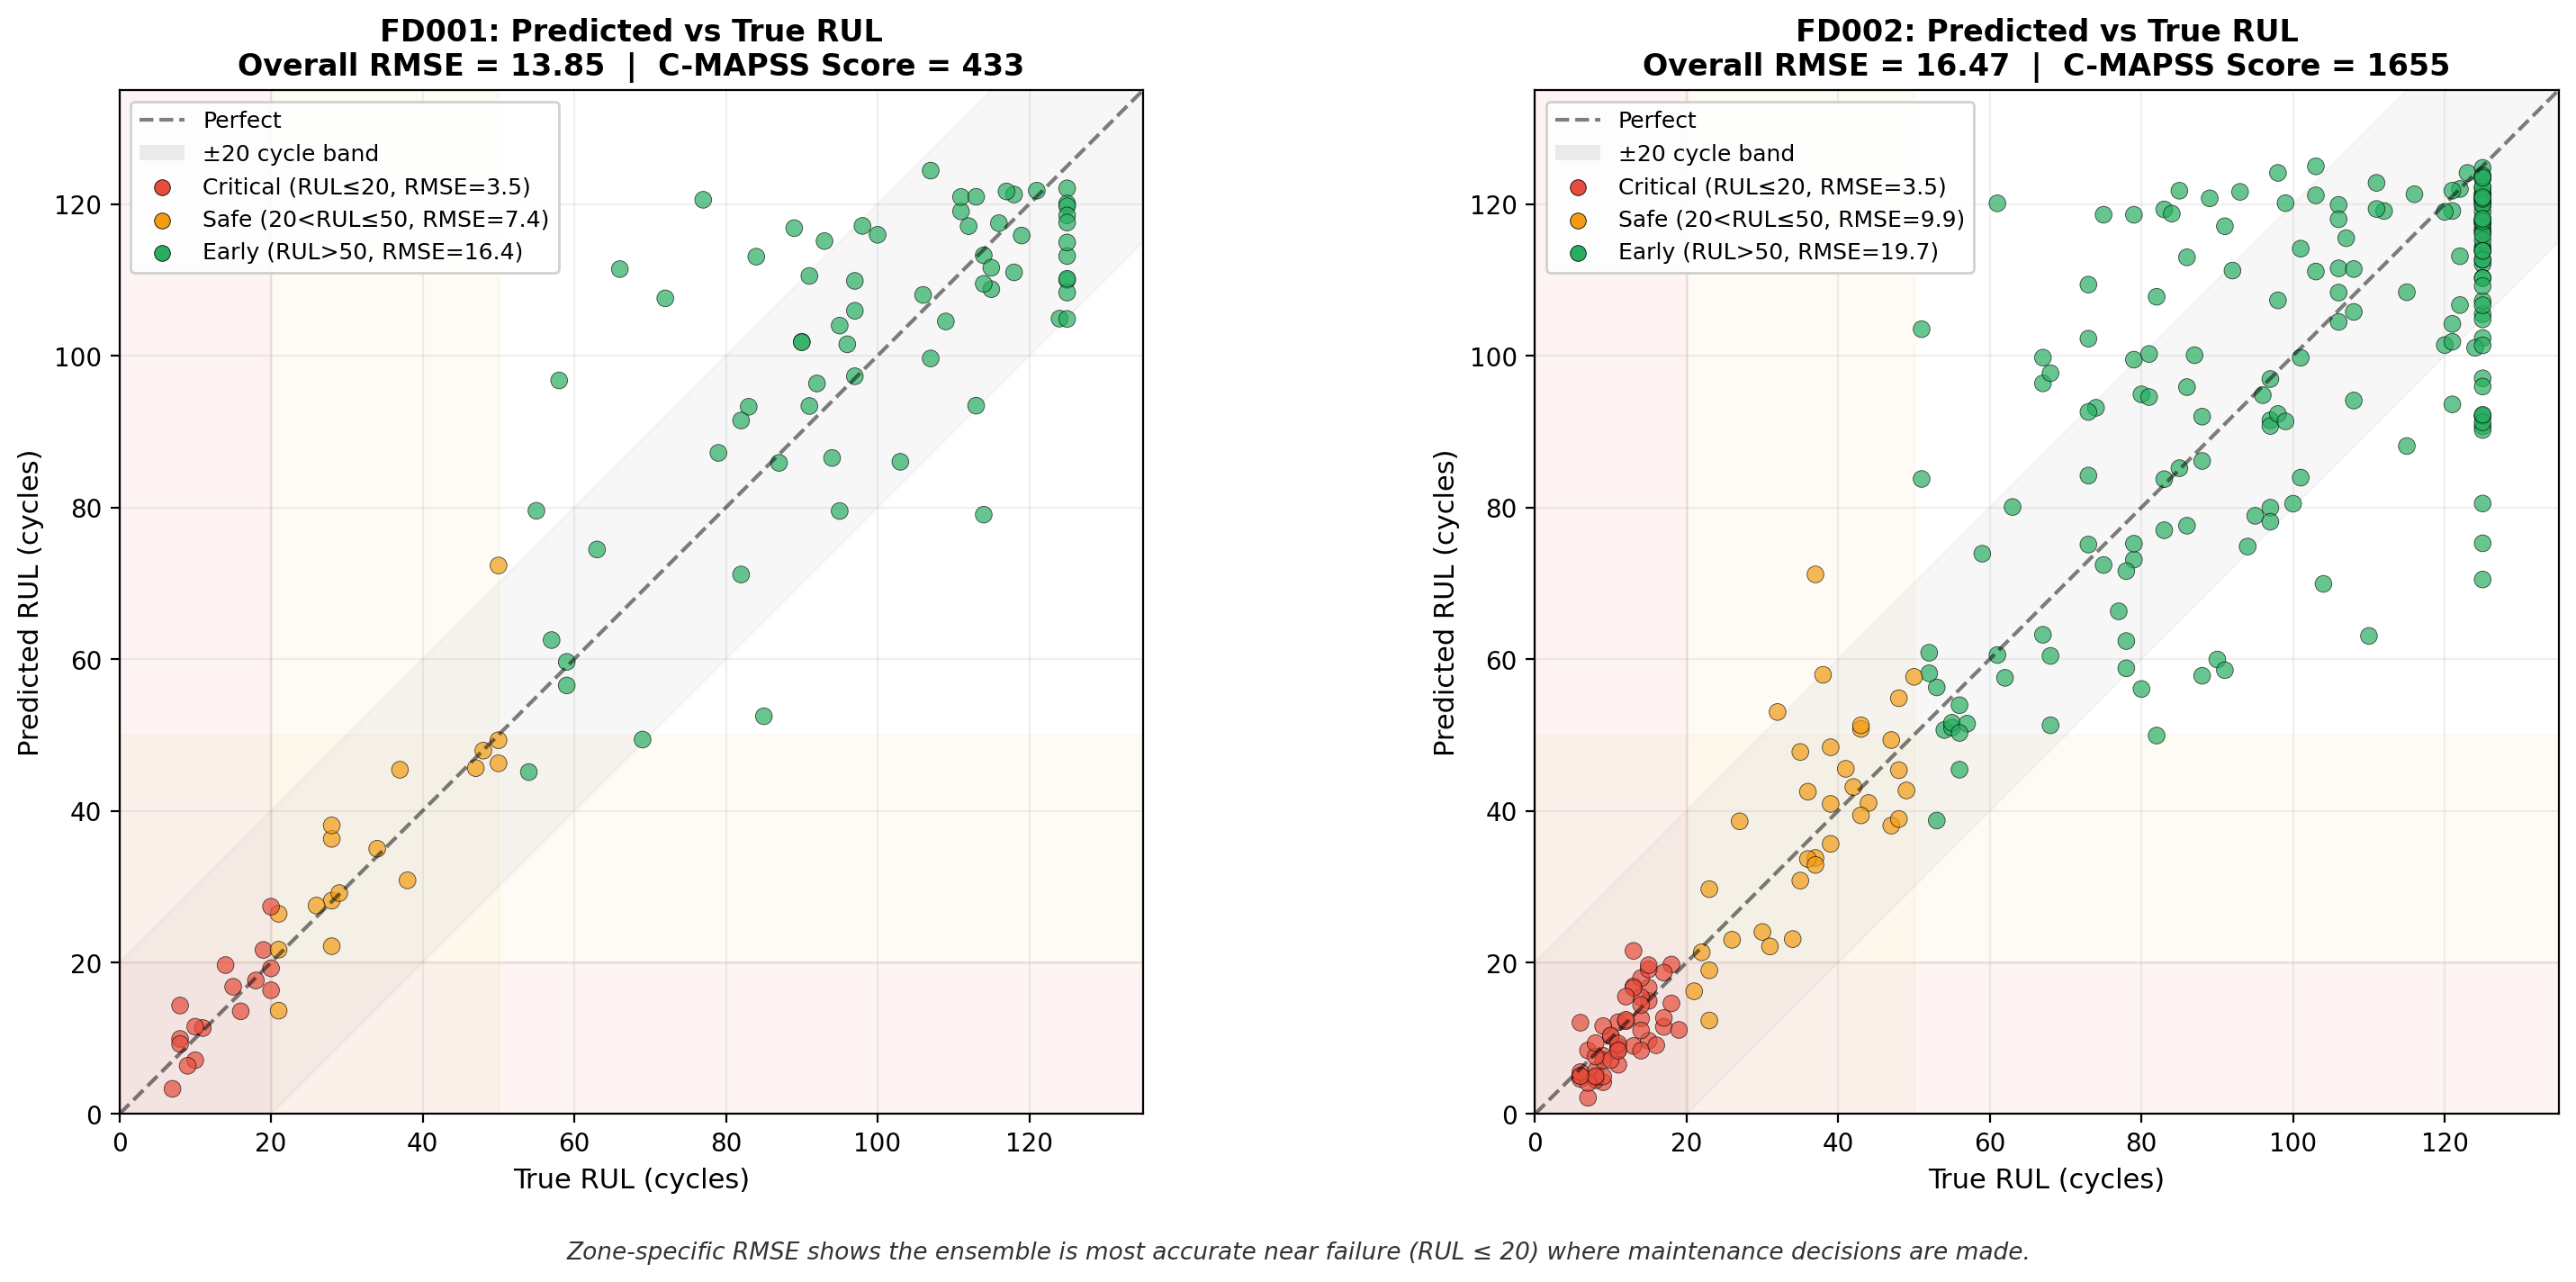
\includegraphics[width=0.85\textwidth]{ensemble_evaluation_1_prediction.png}
\caption{Ensemble mean predicted RUL versus true RUL on the C-MAPSS test set. Points near the diagonal indicate accurate predictions; scatter increases at higher RUL values where early-life degradation is difficult to distinguish.}
\label{fig:ensemble_pred}
\end{figure}

\begin{figure}[h]
\centering
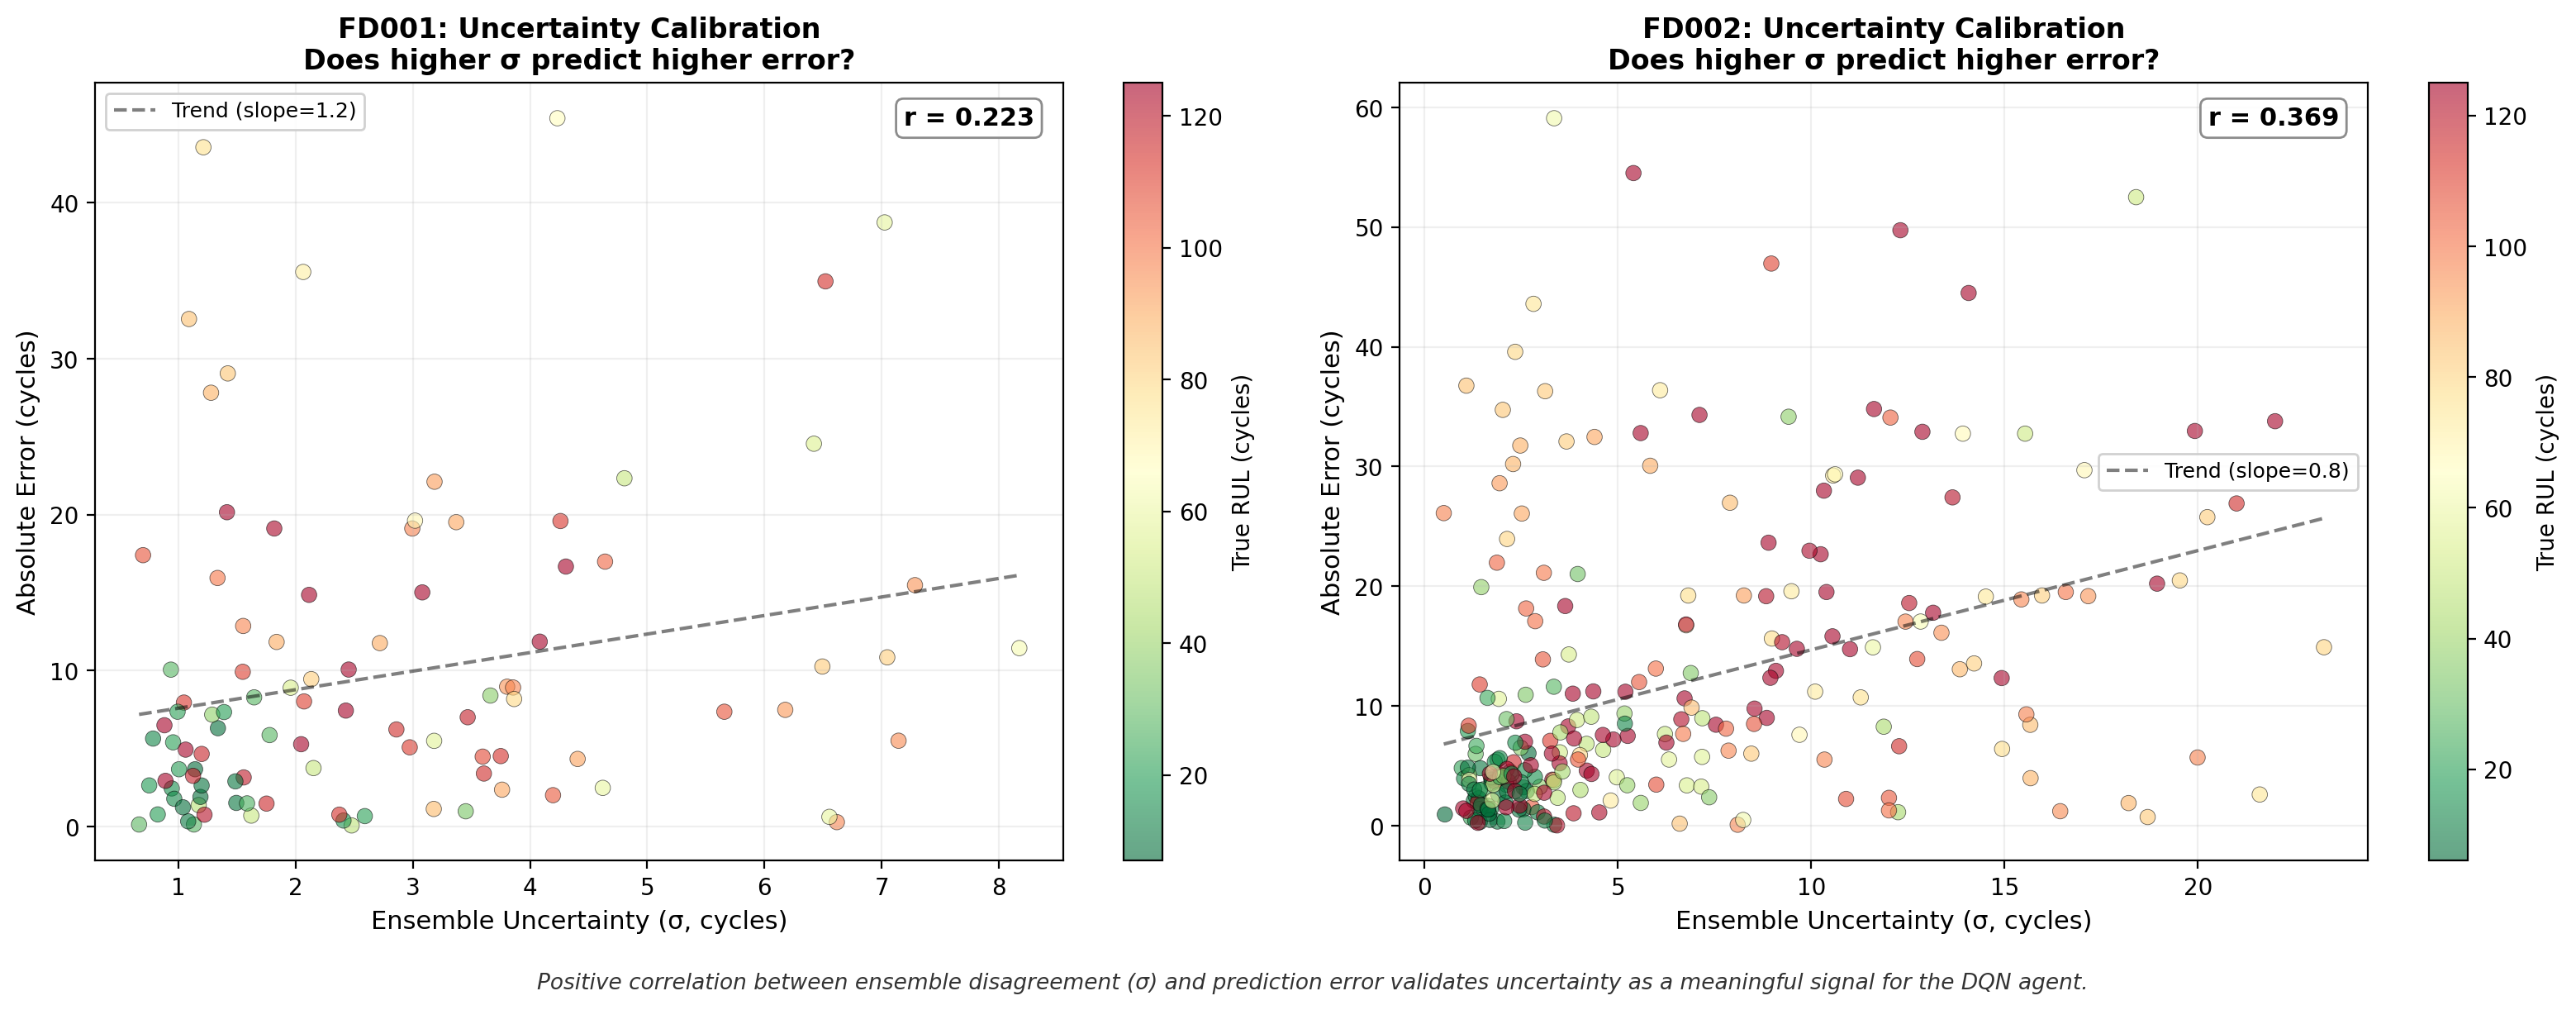
\includegraphics[width=0.85\textwidth]{ensemble_evaluation_3_uncertainty.png}
\caption{Ensemble uncertainty (standard deviation across five members) as a function of prediction error. Higher disagreement among ensemble members correlates with larger prediction errors, validating the use of ensemble disagreement as a proxy for prediction reliability.}
\label{fig:ensemble_uncertainty}
\end{figure}

\section{Reinforcement Learning for Predictive Maintenance}

With a reliable RUL prediction and a meaningful uncertainty signal, the remaining challenge is to make optimal maintenance decisions. This section reviews how reinforcement learning has been applied to the maintenance scheduling problem, evaluates the merits of different RL algorithms, and identifies the gaps that motivated the approach taken in this project.

\subsection{Maintenance as a Markov Decision Process}

The predictive maintenance scheduling problem can be naturally formulated as a Markov Decision Process (MDP), where an agent observes the current engine state, selects an action (typically wait or perform maintenance), and receives a reward or penalty reflecting the quality of that decision. The Markov property is satisfied when the observation includes sufficient information about the current degradation state, which is why this project included four dimensions: the ensemble mean RUL prediction, instantaneous uncertainty, rolling average uncertainty, and a sensor trend signal.


\citet{zhang2019deep} pioneered the application of Deep Q-Networks to predictive maintenance on C-MAPSS, formulating a simple two-action MDP where the agent observed the predicted RUL and selected wait or maintain. They showed that the DQN learned to schedule maintenance in the late degradation phase, outperforming fixed-threshold baselines. However, their formulation used a single-model RUL prediction with no uncertainty quantification, leaving the agent unable to distinguish between confident and unreliable predictions.

\subsection{Deep Q-Networks}

The Deep Q-Network (DQN), introduced by \citet{mnih2015human} for Atari game play, approximates the optimal action-value function $Q^*(s,a)$ using a neural network. The agent selects the action with the highest estimated Q-value for the current state, and updates the network by minimising the temporal-difference error between predicted and target Q-values. Key architectural innovations including experience replay and target networks stabilised training and enabled DQN to achieve human-level performance on a range of tasks.


DQN was selected over policy gradient methods because the discrete two-action space is precisely where value-based methods are most efficient, experience replay allows learning from expensive ensemble-inference transitions multiple times, and Stable-Baselines3 \citep{raffin2021stable} provides a well-tested implementation.

\subsection{Alternative RL Approaches}

Policy gradient methods (PPO \citep{schulman2017proximal}, SAC \citep{haarnoja2018soft}) are better suited to continuous or high-dimensional action spaces and offer no advantage for discrete two-action problems. Model-based RL could improve sample efficiency but would require learning degradation dynamics, adding complexity without clear benefit given the existing LSTM ensemble.

\subsection{Noise Augmentation and Domain Randomisation}

A key contribution of this project was training the RL agent under augmented noise conditions so that it learned to interpret the uncertainty signal from the LSTM ensemble. This approach draws on the broader concept of domain randomisation, originally proposed for sim-to-real transfer in robotics by \citet{tobin2017domain}. The core idea is that if an agent trains under a wide distribution of environmental conditions, it will learn policies that are robust to the specific conditions encountered at deployment.


In the context of predictive maintenance, \citet{wang2020remaining} showed that adding Gaussian noise to sensor inputs during training improved the generalisation of RUL prediction models to noisy test conditions. This project extended that principle from the prediction layer to the decision layer: during 70\% of training episodes, Gaussian noise was injected into the raw sensor data before ensemble inference, causing ensemble disagreement to rise. The DQN agent thus encountered varying noise levels during training and learned that a high uncertainty observation indicates unreliable predictions that warrant more cautious behaviour. To the best of the author's knowledge, no prior work has combined noise-augmented RL training with ensemble uncertainty as an explicit observation signal for maintenance scheduling.

\section{Safety Mechanisms in Autonomous Decision Systems}

Any system that makes high-stakes decisions autonomously must include safeguards against catastrophic failure. This is particularly true in the aerospace domain, where a wrong maintenance decision can have severe consequences. This section reviews the approaches to ensuring safety in autonomous systems and positions the safety supervisor developed in this project within that context.

\subsection{Safe Reinforcement Learning}

Safe RL seeks to ensure learned policies satisfy constraints \citep{garcia2015comprehensive}. Constrained MDP approaches \citep{tessler2018reward} are theoretically elegant but add complexity and may still violate constraints during training. Shielding approaches provide hard guarantees by interposing a deterministic override; \citet{alshiekh2018safe} formalised this as a safety shield that replaces unsafe actions with safe defaults. This project adopted the shielding approach: the safety supervisor overrides the DQN agent when the ensemble confidently predicts imminent failure.

\subsection{Hierarchical Safety Architectures}

Aerospace safety standard DO-178C mandates multiple independent protection layers \citep{do178c}, aligning naturally with the three-layer architecture. \citet{amodei2016concrete} identified robustness to distributional shift as a core AI safety problem. The two-tier safety supervisor addresses this directly: even if the ensemble's uncertainty estimate becomes unreliable, the hard critical threshold provides a final line of defence.

\subsection{Uncertainty-Aware Safety}

A growing body of work has explored using prediction uncertainty as a trigger for cautious behaviour. \citet{michelmore2020uncertainty} used epistemic uncertainty as a safety signal in autonomous driving, triggering a handover to a human operator when the perception model's uncertainty exceeded a threshold. \citet{lutjens2019safe} proposed a safe RL framework for autonomous navigation where the agent's action was constrained when a Bayesian neural network reported high uncertainty about the environment state. More recently, \citet{liu2023safe} extended uncertainty-aware exploration to autonomous systems with formal safety constraints, demonstrating that uncertainty-guided action selection can reduce constraint violations during both training and deployment. \citet{chen2024uncertainty} applied deep ensemble uncertainty to industrial predictive maintenance decisions, providing independent validation that ensemble disagreement is an effective signal for maintenance timing. These works validate the principle that uncertainty can serve as an effective safety signal, though none have combined all three elements (ensemble uncertainty as RL observation, noise-augmented training, and a deterministic safety supervisor) within a single integrated framework as this project does.


The safety supervisor in this project is novel in its specific two-tier design for the predictive maintenance context. The uncertainty-aware tier engages when the ensemble is confident in a low-RUL prediction (i.e., low rolling standard deviation combined with a prediction below the critical threshold), while the hard critical tier fires unconditionally at very low RUL regardless of uncertainty. This asymmetric design recognises that high uncertainty should make the system less confident in its override decision, not more, a subtlety that most existing safety mechanisms do not capture.

\section{Synthesis and Research Gaps}

The literature reviewed above reveals four distinct research communities, prediction, uncertainty, decision-making, and safety, that have each made significant progress in isolation but have rarely been integrated into a single coherent system. Table~\ref{tab:lit_gaps} summarises the key gaps identified.


\begin{table}[h]
\centering
\caption{Summary of identified research gaps and how this project addresses each one.}
\label{tab:lit_gaps}
\renewcommand{\arraystretch}{1.4}
\begin{tabular}{>{\raggedright\arraybackslash}p{3.2cm} >{\raggedright\arraybackslash}p{5.8cm} >{\raggedright\arraybackslash}p{4.5cm}}
\toprule
\textbf{Research Gap} & \textbf{Description} & \textbf{How This Project Addresses It} \\
\midrule
Prediction-to-decision disconnect & Most RUL research optimises prediction accuracy without considering how predictions translate into maintenance actions. & The LSTM ensemble feeds directly into a DQN agent that learns \emph{when} to act, not just how to predict. \\
\addlinespace
Uncertainty treated as diagnostic only & Where uncertainty is quantified, it is used as a post-hoc diagnostic rather than as an input to downstream decision-making. & Ensemble disagreement is an explicit dimension of the agent's observation space. \\
\addlinespace
RL without uncertainty awareness & Existing RL-based maintenance systems observe the predicted RUL but not the model's confidence in that prediction. & The DQN agent observes both instantaneous and rolling uncertainty signals alongside the RUL prediction. \\
\addlinespace
Safety as an afterthought & Safety mechanisms are rarely integrated into the RL evaluation; most work assumes the agent will learn safe behaviour on its own. & A two-tier deterministic safety supervisor provides an explicit override safeguard, evaluated as a formal ablation layer. \\
\addlinespace
No robustness evaluation under sensor degradation & Evaluation is almost always conducted on clean test data; very few studies systematically vary sensor noise. & All experiments are repeated across eight noise levels (0.000--0.175) with 500 episodes per condition. \\
\bottomrule
\end{tabular}
\end{table}


This project was designed to address all five gaps simultaneously. A deep LSTM ensemble (Section~2.2) provided both RUL predictions and a calibrated uncertainty signal. That uncertainty signal was fed directly into a DQN agent (Section~2.3) as part of its observed state, and the agent was trained under noise augmentation so that it learned to condition its behaviour on uncertainty. A two-tier safety supervisor (Section~2.4) provided a deterministic safety backstop independent of the learned policy. Finally, the entire system was evaluated across eight noise levels in a rigorous ablation study, directly testing robustness under the sensor degradation conditions that the literature has largely neglected.


The design principles derived from this review, specifically the choice of LSTM as the prediction backbone, deep ensembles as the uncertainty quantification method, DQN as the RL algorithm, noise augmentation as the training strategy, and a deterministic safety shield as the final safety backstop, are formalised into system requirements in Chapter~3.


\chapter{Requirements Analysis and Design}

This chapter translates the research gaps and design principles identified in the literature review into a concrete set of system requirements and a detailed architectural design. The requirements were derived from three sources: the project objectives defined in Section~1.2, the technical findings of the literature review in Chapter~2, and the practical constraints of the C-MAPSS evaluation environment. Each requirement is prioritised using the MoSCoW framework and traced forward to the design decisions it motivated. The chapter concludes with the complete system architecture, the Markov Decision Process formulation, and the reward structure that governed agent training.

\section{Requirements Elicitation}

Requirements were elicited from four sources: the eight project objectives (Section~1.2), the literature review's state-of-the-art patterns, C-MAPSS dataset constraints (dimensionality, sequence length, ground truth), and practical constraints discovered during iterative prototyping. As the system is a research prototype evaluated by simulation, no user studies were conducted; the requirements reflect functional capabilities and performance thresholds needed for valid experimental results.

\section{Assumptions and Constraints}

The following assumptions and constraints bounded the development and are important for interpreting the experimental results.


\begin{enumerate}[label=\textbf{A\arabic*.}, leftmargin=2cm]
  \item \textbf{Simulated degradation.} The C-MAPSS dataset is a physics-based simulation, not real operational data. Results demonstrate the viability of the approach but do not constitute evidence of real-world deployment readiness. This is a standard limitation shared by the entire C-MAPSS research community \citep{ramasso2014review}.

  \item \textbf{Single-fault-mode subsets.} Only FD001 (single operating condition, single fault mode) and FD002 (six operating conditions, single fault mode) were used. FD003 and FD004, which introduce a second fault mode, were excluded to keep the experimental scope manageable while still testing multi-condition robustness.

  \item \textbf{Gaussian noise model.} Sensor degradation was modelled as additive Gaussian noise with zero mean, which is the standard assumption in the literature \citep{wang2020remaining}. Real sensor failures can exhibit bias, drift, and intermittent dropout, which would require a richer noise model.

  \item \textbf{Binary action space.} The agent's decision was restricted to two actions: wait or perform maintenance. Real-world maintenance scheduling involves graduated responses (inspection, partial repair, full overhaul) and multi-engine fleet coordination, which are beyond the scope of this project.

  \item \textbf{Computational resources.} Training was performed on a single consumer GPU. This constrained the ensemble size to five members and the DQN training to 1.5 million timesteps. Larger ensembles and longer training could improve performance but were not feasible within the available resources.

  \item \textbf{RUL cap at 125 cycles.} Following the convention established by \citet{heimes2008recurrent}, the maximum RUL was capped at 125 cycles. This means the system does not attempt to distinguish between engines at 200 and 300 cycles remaining; both are treated as ``healthy.''
\end{enumerate}

\section{Functional Requirements}

Table~\ref{tab:func_req} presents the functional requirements, prioritised using the MoSCoW framework. Must-have requirements define the minimum viable system needed to test the core hypothesis (that uncertainty awareness improves maintenance decisions). Should-have requirements strengthen the experimental rigour. Could-have requirements add value but are not essential to the core contribution.


\begin{table}[h]
\centering
\small
\caption{Functional requirements prioritised using MoSCoW.}
\label{tab:func_req}
\renewcommand{\arraystretch}{1.3}
\setlength{\tabcolsep}{4pt}
\begin{tabular}{>{\raggedright\arraybackslash}p{0.8cm} >{\raggedright\arraybackslash}p{1.5cm} >{\raggedright\arraybackslash}p{8.5cm} >{\raggedright\arraybackslash}p{2cm}}
\toprule
\textbf{ID} & \textbf{Priority} & \textbf{Requirement} & \textbf{Objective} \\
\midrule
FR1 & Must & The system shall load, preprocess, and normalise C-MAPSS FD001 and FD002 data with a RUL cap of 125 cycles. & Obj.~1 \\
FR2 & Must & The system shall train an ensemble of five LSTM networks on bootstrap samples and produce per-cycle RUL predictions with an ensemble disagreement uncertainty signal. & Obj.~2 \\
FR3 & Must & The system shall implement a Gymnasium-compatible environment where an agent observes a four-dimensional state (mean RUL, instantaneous $\sigma$, rolling $\sigma$, sensor trend) and selects WAIT or MAINTAIN. & Obj.~3 \\
FR4 & Must & The system shall train a DQN agent with noise augmentation (70\% of episodes) and produce a trained uncertainty-aware policy. & Obj.~4 \\
FR5 & Must & The system shall train a blind DQN agent with the uncertainty signal zeroed out, serving as a controlled ablation baseline. & Obj.~4 \\
FR6 & Must & The system shall implement a two-tier safety supervisor that overrides the agent's action when the ensemble confidently predicts imminent failure. & Obj.~5 \\
FR7 & Must & The system shall evaluate both agents across eight noise levels with 500 episodes per condition and report statistical significance (Welch's t-test) and effect size (Cohen's d). & Obj.~6 \\
\addlinespace
FR8 & Should & The system shall compute fleet-level cost projections for a 50-engine fleet under both agent strategies. & Obj.~7 \\
FR9 & Should & The system shall compare the DQN agent against multiple fixed-threshold baselines to verify that the learned policy is non-trivial. & Obj.~6 \\
FR10 & Should & The system shall produce publication-quality figures for all experimental results. & Obj.~6 \\
\addlinespace
FR11 & Could & The system shall provide an interactive Streamlit dashboard for real-time cycle-by-cycle demonstration. & Obj.~8 \\
FR12 & Could & The dashboard shall allow users to toggle between uncertainty-aware and blind agents, enable/disable the safety supervisor, and inject noise at adjustable intensities. & Obj.~8 \\
\bottomrule
\end{tabular}
\end{table}

\section{Non-Functional Requirements}

Table~\ref{tab:nonfunc_req} presents the non-functional requirements. These ensure that the system produces valid experimental results and is usable for demonstration purposes.


\begin{table}[h]
\centering
\small
\caption{Non-functional requirements prioritised using MoSCoW.}
\label{tab:nonfunc_req}
\renewcommand{\arraystretch}{1.3}
\setlength{\tabcolsep}{4pt}
\begin{tabular}{>{\raggedright\arraybackslash}p{0.8cm} >{\raggedright\arraybackslash}p{1.5cm} >{\raggedright\arraybackslash}p{9cm} >{\raggedright\arraybackslash}p{1.5cm}}
\toprule
\textbf{ID} & \textbf{Priority} & \textbf{Requirement} & \textbf{Source} \\
\midrule
NF1 & Must & All experiments shall be reproducible via fixed random seeds across runs. & Lit.~review \\
NF2 & Must & Ensemble inference (five forward passes) shall complete within 100ms per cycle on commodity hardware to support real-time dashboard operation. & Design \\
NF3 & Must & The system shall use a centralised configuration file so that all hyperparameters (LSTM, DQN, noise, safety thresholds) can be modified without code changes. & Best practice \\
NF4 & Should & The codebase shall be modular, with separate modules for preprocessing, model definition, Gymnasium environment, and configuration. & Best practice \\
NF5 & Should & Statistical tests shall report 95\% confidence intervals alongside point estimates. & Lit.~review \\
NF6 & Could & The Streamlit dashboard shall render at a minimum of 10 frames per second for the cycle-by-cycle animation. & Usability \\
\bottomrule
\end{tabular}
\end{table}

\section{System Architecture}

The architecture was designed as three loosely coupled layers, each fulfilling a distinct role in the decision pipeline. This separation of concerns was motivated by two findings from the literature: first, that prediction and decision-making benefit from independent optimisation \citep{zhang2019deep}; and second, that safety guarantees are most robust when provided by a deterministic module rather than a learned one \citep{alshiekh2018safe}. Figure~\ref{fig:arch} provides a high-level overview.


\begin{figure}[h]
\centering
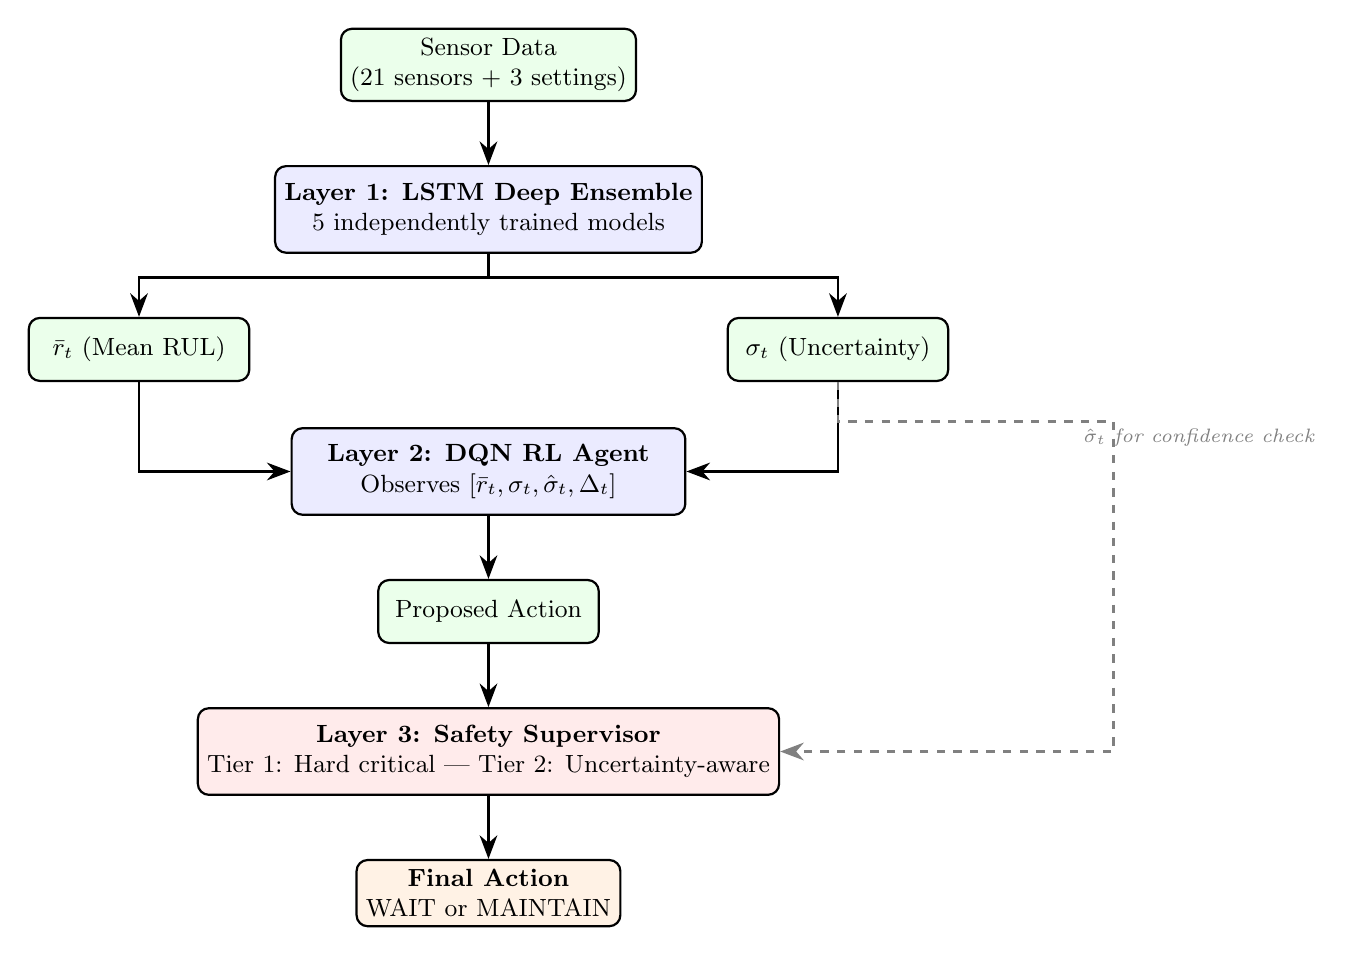
\begin{tikzpicture}[
    node distance=0.8cm and 1.5cm,
    box/.style={rectangle, draw, rounded corners, minimum width=3.2cm, minimum height=1.1cm, align=center, font=\small},
    layer/.style={box, fill=blue!8, line width=0.8pt},
    data/.style={box, fill=green!8, line width=0.8pt, minimum width=2.8cm, minimum height=0.8cm},
    action/.style={box, fill=orange!10, line width=0.8pt, minimum width=2.8cm, minimum height=0.8cm},
    arrow/.style={-{Stealth[length=3mm]}, thick},
    label/.style={font=\scriptsize\itshape, text=gray}
]
    % Sensor input
    \node[data] (sensors) {Sensor Data\\(21 sensors + 3 settings)};

    % Layer 1
    \node[layer, below=0.8cm of sensors, minimum width=5cm] (ensemble) {\textbf{Layer 1: LSTM Deep Ensemble}\\5 independently trained models};

    % Outputs of Layer 1
    \node[data, below left=0.8cm and 0.3cm of ensemble] (rul) {$\bar{r}_t$ (Mean RUL)};
    \node[data, below right=0.8cm and 0.3cm of ensemble] (sigma) {$\sigma_t$ (Uncertainty)};

    % Layer 2
    \node[layer, below=2.2cm of ensemble, minimum width=5cm] (dqn) {\textbf{Layer 2: DQN RL Agent}\\Observes $[\bar{r}_t, \sigma_t, \hat{\sigma}_t, \Delta_t]$};

    % Proposed action
    \node[data, below=0.8cm of dqn] (proposed) {Proposed Action};

    % Layer 3
    \node[layer, below=0.8cm of proposed, minimum width=5cm, fill=red!8] (safety) {\textbf{Layer 3: Safety Supervisor}\\Tier 1: Hard critical | Tier 2: Uncertainty-aware};

    % Final action
    \node[action, below=0.8cm of safety] (final) {\textbf{Final Action}\\WAIT or MAINTAIN};

    % Arrows
    \draw[arrow] (sensors) -- (ensemble);
    \draw[arrow] (ensemble.south) -- ++(0,-0.3) -| (rul.north);
    \draw[arrow] (ensemble.south) -- ++(0,-0.3) -| (sigma.north);
    \draw[arrow] (rul.south) |- (dqn.west);
    \draw[arrow] (sigma.south) |- (dqn.east);
    \draw[arrow] (dqn) -- (proposed);
    \draw[arrow] (proposed) -- (safety);
    \draw[arrow] (safety) -- (final);

    % Feedback arrow for sigma to safety
    \draw[arrow, dashed, gray] (sigma.south) -- ++(0,-0.5) -- ++(3.5,0) |- (safety.east);
    \node[label, right] at ($(sigma.south)+(3.0,-0.7)$) {$\hat{\sigma}_t$ for confidence check};

\end{tikzpicture}
\caption{Three-layer system architecture. Sensor data flows through the LSTM deep ensemble (Layer~1), which produces both a mean RUL prediction and an uncertainty signal. Both are observed by the DQN agent (Layer~2), whose proposed action is subject to the safety supervisor's (Layer~3) two-tier override logic before execution. The dashed line indicates the uncertainty signal also feeding into the supervisor's confidence check.}
\label{fig:arch}
\end{figure}

\subsection{Layer 1: LSTM Deep Ensemble}

The prediction layer comprised five independently trained LSTM networks. LSTM was selected because RUL forecasting is sequential and requires modelling temporal dependencies in non-linear degradation trajectories \citep{hochreiter1997long, zheng2017long}. For the available dataset size and real-time inference constraints, a compact LSTM offered a practical trade-off versus heavier alternatives \citep{wu2018remaining, zhang2022transformer}. Each network consisted of a two-layer LSTM with hidden dimension 100 and dropout 0.2, followed by a linear output layer producing scalar RUL from the last hidden state. Inputs were 30-cycle windows of 24 features, and RUL targets were normalised by the 125-cycle cap.


Diversity among ensemble members was achieved through bootstrap sampling: each model was trained on a random 80\% subset with replacement, following \citet{fort2019deep}. Deep ensembles were selected for uncertainty because they are practical and well-calibrated under shift compared with lighter approximations such as MC Dropout \citep{lakshminarayanan2017simple, ovadia2019can}. At inference time, the ensemble produced two signals for each cycle: mean prediction and standard deviation:
\begin{equation}
\bar{r}_t = \frac{1}{M}\sum_{m=1}^{M} r_t^{(m)}, \quad
\sigma_t = \sqrt{\frac{1}{M-1}\sum_{m=1}^{M}\left(r_t^{(m)}-\bar{r}_t\right)^2}
\end{equation}
The standard deviation was scaled by a factor of 15 (determined empirically during development) to map the raw range of approximately 0.01--0.10 into a range that was informative for the downstream DQN agent.


Figure~\ref{fig:ensemble_error} illustrates the distribution of prediction errors grouped by RUL zone, showing that the ensemble achieves tight error distributions in the critical end-of-life region where maintenance decisions are most consequential.

\begin{figure}[h]
\centering
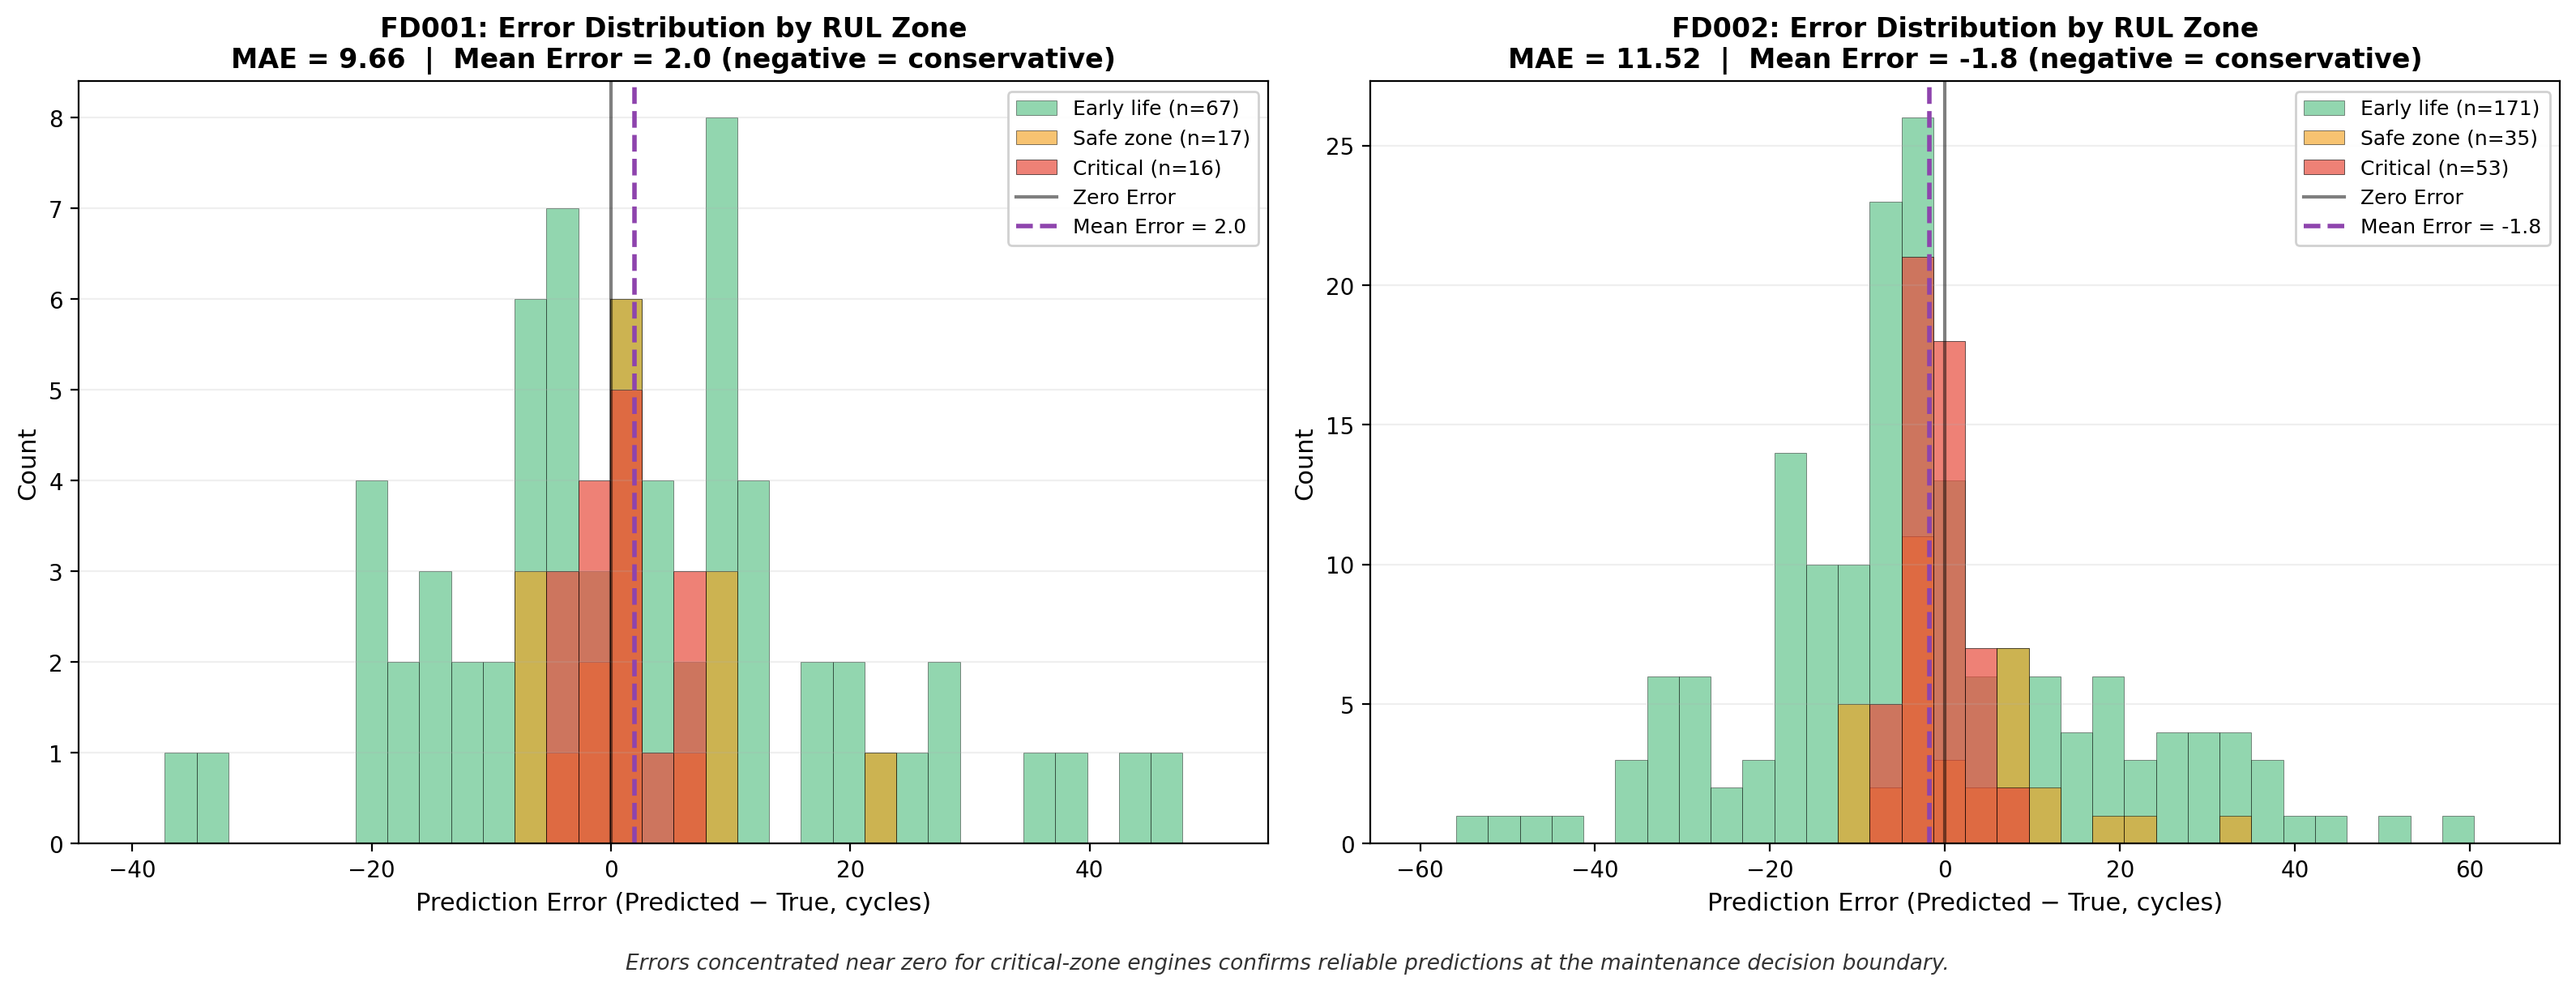
\includegraphics[width=0.85\textwidth]{ensemble_evaluation_2_error.png}
\caption{Distribution of ensemble prediction errors across different RUL zones. Errors are tightest in the critical low-RUL region (0--25 cycles), where prediction accuracy matters most for maintenance scheduling.}
\label{fig:ensemble_error}
\end{figure}

\subsection{Layer 2: Deep Q-Network Agent}

The decision layer was formulated as a Markov Decision Process and solved using a DQN agent. The MDP components are defined below.


\textbf{State space.} The agent observed a four-dimensional continuous state at each engine cycle:
\begin{equation}
s_t = \begin{bmatrix} \bar{r}_t, \quad \sigma_t, \quad \hat{\sigma}_t, \quad \Delta_t \end{bmatrix}
\end{equation}
where $\bar{r}_t$ is the ensemble mean normalised RUL prediction, $\sigma_t$ is the instantaneous scaled ensemble standard deviation, $\hat{\sigma}_t$ is a rolling average of $\sigma_t$ over the preceding 3 cycles (providing a smoothed uncertainty trend), and $\Delta_t$ is a sensor trend signal derived from the rate of change in the ensemble prediction over recent cycles. For the blind ablation agent, $\sigma_t$ and $\hat{\sigma}_t$ were set to zero, removing all uncertainty information from the observation while keeping the state dimensionality identical.


\textbf{Action space.} $\mathcal{A} = \{0, 1\}$, where action 0 is WAIT (continue operating) and action 1 is MAINTAIN (schedule maintenance immediately, ending the episode).


\textbf{Transition dynamics.} At each step, the environment advanced by one engine cycle. The next sensor readings were drawn from the C-MAPSS dataset, optionally corrupted with Gaussian noise during training episodes (with probability 0.7 and noise standard deviation sampled uniformly from 0.02 to 0.20). The LSTM ensemble then produced updated predictions and uncertainty estimates for the new cycle. If the true RUL reached zero before the agent chose MAINTAIN, the engine was considered to have crashed.


\textbf{Reward function.} The reward structure, summarised in Table~\ref{tab:reward}, was designed to encode the asymmetric costs of maintenance timing:

\begin{table}[h]
\centering
\caption{Reward function for the predictive maintenance MDP.}
\label{tab:reward}
\renewcommand{\arraystretch}{1.3}
\begin{tabular}{>{\raggedright\arraybackslash}p{2.5cm} >{\raggedright\arraybackslash}p{3cm} >{\raggedright\arraybackslash}p{7cm}}
\toprule
\textbf{Action} & \textbf{Condition} & \textbf{Reward} \\
\midrule
MAINTAIN & True RUL $< 20$ & $+500$ \quad (jackpot: optimal timing) \\
MAINTAIN & True RUL $\in [20, 50)$ & $+10$ \quad\;\; (safe but early) \\
MAINTAIN & True RUL $\geq 50$ & $-20$ \quad\;\; (wasteful: too early) \\
\addlinespace
WAIT & True RUL $>$ 25 & $+1$ \quad\;\;\;\, (normal operation) \\
WAIT & True RUL $\leq$ 25 & $+1 - \text{time pressure}$ \quad (linearly decaying) \\
WAIT & High $\sigma$ in buffer zone & $-\text{uncertainty urgency penalty}$ \\
\addlinespace
(crash) & Engine crashes (RUL = 0) & $-500$ \quad (catastrophic failure) \\
\bottomrule
\end{tabular}
\end{table}


The jackpot reward of $+500$ for maintaining within the last 20 cycles was set deliberately high to dominate the discounted sum of WAIT rewards, ensuring that the agent learned to pursue optimal timing rather than risk-averse early maintenance. The crash penalty of $-500$ created a symmetric incentive: failing to act was as costly as acting optimally was beneficial. The time-pressure shaping caused the WAIT reward to decay linearly once the true RUL dropped below 25 cycles, preventing the agent from learning a ``wait forever'' policy. An uncertainty urgency penalty was applied when the agent chose WAIT while both the predicted RUL was in the buffer zone (between 20 and 50 cycles) and the scaled uncertainty was high, encouraging the agent to act cautiously under unreliable predictions. A proactive maintenance bonus of $+30$ was additionally awarded for maintaining under high uncertainty in the buffer zone, reinforcing that uncertain situations near end-of-life warrant action rather than inaction.


\textbf{DQN architecture and training.} The Q-network was a fully connected network with three hidden layers of 256, 256, and 128 neurons. Training used the Adam optimiser with a learning rate of $3 \times 10^{-4}$, a replay buffer of 150,000 transitions, a discount factor $\gamma = 0.99$, and an $\epsilon$-greedy exploration schedule that decayed from 1.0 to 0.03 over 40\% of the 1.5 million training timesteps. To address the class imbalance inherent in the problem (most of an engine's life is spent in the healthy phase where no maintenance decision matters), 60\% of training episodes were initialised near end-of-life, within the last 50 cycles of a randomly selected engine trajectory. This end-of-life bias ensured that the agent encountered a sufficient number of critical decision points during training.


DQN was chosen over PPO because the action space is binary (WAIT/MAINTAIN), where value-based learning with replay and target networks is sample-efficient and stable \citep{mnih2015human}. PPO remained a valid alternative, but its on-policy updates are typically less sample-efficient in this setting \citep{schulman2017proximal}. The core DQN target and loss are:
\begin{equation}
y_t = r_t + \gamma \max_{a'}Q_{\theta^-}(s_{t+1}, a'), \qquad
\mathcal{L}(\theta)=\mathbb{E}\left[(Q_{\theta}(s_t,a_t)-y_t)^2\right]
\end{equation}

\subsection{Layer 3: Safety Supervisor}

The safety supervisor implemented a deterministic two-tier override that operated after the DQN agent proposed an action and before that action was executed in the environment.


\textbf{Tier 1: Hard critical override.} If the ensemble mean prediction $\bar{r}_t < 0.04$ (approximately 5 cycles remaining), the supervisor forced MAINTAIN \emph{unconditionally}, regardless of the uncertainty level. This tier served as a final safety net for scenarios where extreme noise caused the rolling uncertainty to exceed the confidence threshold, which would otherwise silence Tier~2 when it was needed most.


\textbf{Tier 2: Uncertainty-aware override.} If the ensemble mean prediction $\bar{r}_t < 0.12$ (approximately 15 cycles remaining) \emph{and} the rolling uncertainty $\hat{\sigma}_t < 0.55$ (indicating that the ensemble was confident in this low prediction), the supervisor overrode the agent's action to MAINTAIN regardless of what the agent proposed. The uncertainty condition was critical: it prevented the supervisor from firing on noisy dips in the prediction that did not reflect genuine degradation.

The two-tier design encoded an important asymmetry. At moderately low RUL values, the supervisor deferred to the DQN agent when uncertainty was high, trusting that the agent's uncertainty-aware training equipped it to handle ambiguous situations. At extremely low RUL values, no amount of uncertainty justified further waiting, and the hard override provided a deterministic last-resort intervention. This design was directly informed by the shielding literature reviewed in Section~2.4 and the defence-in-depth principle mandated by aerospace safety standards \citep{do178c}.


Figure~\ref{fig:supervisor_flow} summarises the Layer~3 decision logic in compact form. This flow makes clear that the supervisor does not replace the DQN policy; it only intercepts decisions when the engine enters either the hard-critical zone or the confidence-gated low-RUL zone.

\begin{figure}[h]
\centering
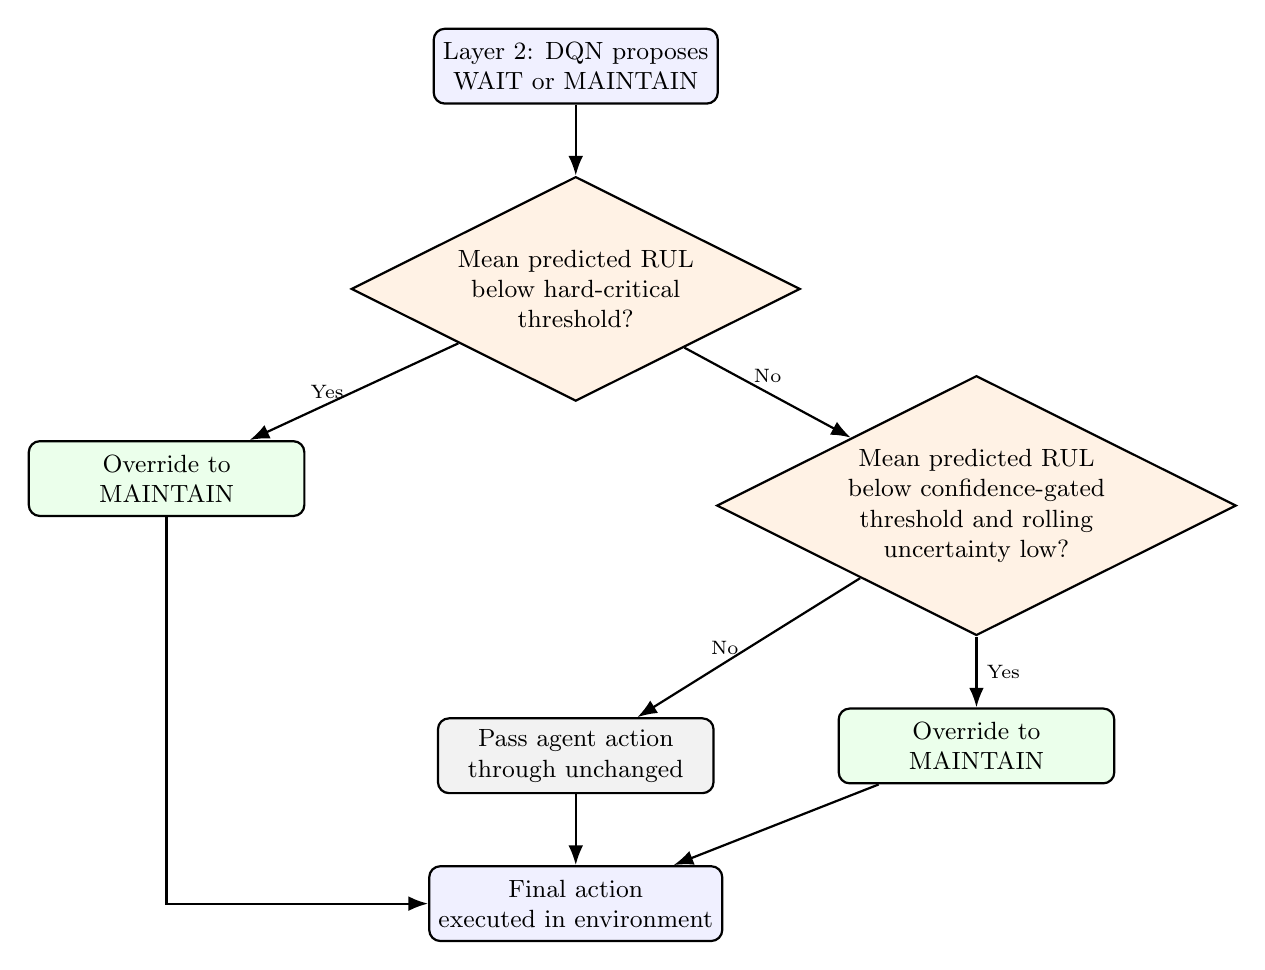
\begin{tikzpicture}[
  node distance=9mm and 11mm,
  every node/.style={font=\small},
  block/.style={rectangle, rounded corners, draw=black, thick, align=center, minimum width=3.2cm, minimum height=0.95cm, fill=blue!6},
  decision/.style={diamond, draw=black, thick, align=center, aspect=2.0, inner sep=1.5pt, fill=orange!10, text width=3.4cm},
  outcome/.style={rectangle, rounded corners, draw=black, thick, align=center, minimum width=3.5cm, minimum height=0.95cm, fill=green!8},
  pass/.style={rectangle, rounded corners, draw=black, thick, align=center, minimum width=3.5cm, minimum height=0.95cm, fill=gray!10},
  line/.style={-{Latex[length=2.5mm]}, thick}
]
\node[block] (start) {Layer 2: DQN proposes\\WAIT or MAINTAIN};
\node[decision, below=of start] (hard) {Mean predicted RUL\\below hard-critical\\threshold?};
\node[outcome, below left=12mm and 20mm of hard] (force1) {Override to\\MAINTAIN};
\node[decision, below right=12mm and 20mm of hard] (conf) {Mean predicted RUL\\below confidence-gated\\threshold and rolling\\uncertainty low?};
\node[outcome, below=of conf] (force2) {Override to\\MAINTAIN};
\node[pass, below=of hard, yshift=-31mm] (pass) {Pass agent action\\through unchanged};
\node[block, below=of pass] (end) {Final action\\executed in environment};

\draw[line] (start) -- (hard);
\draw[line] (hard) -- node[left, font=\scriptsize] {Yes} (force1);
\draw[line] (hard) -- node[above, font=\scriptsize] {No} (conf);
\draw[line] (conf) -- node[right, font=\scriptsize] {Yes} (force2);
\draw[line] (conf) -- node[left, font=\scriptsize] {No} (pass);
\draw[line] (force1) |- (end);
\draw[line] (force2) -- (end);
\draw[line] (pass) -- (end);
\end{tikzpicture}
\caption{Safety supervisor decision flow. The DQN agent always proposes the action first. Layer~3 only overrides that proposal in two cases: an unconditional hard-critical state, or a low-RUL state where rolling uncertainty indicates that the ensemble is sufficiently confident in its prediction.}
\label{fig:supervisor_flow}
\end{figure}


To illustrate how the three layers operate in concert during a single engine lifecycle, Figure~\ref{fig:engine_timeline} presents a representative timeline showing the ensemble prediction, the uncertainty signal, and the agent's decision pressure evolving cycle by cycle as an engine approaches end of life.

\begin{figure}[h]
\centering
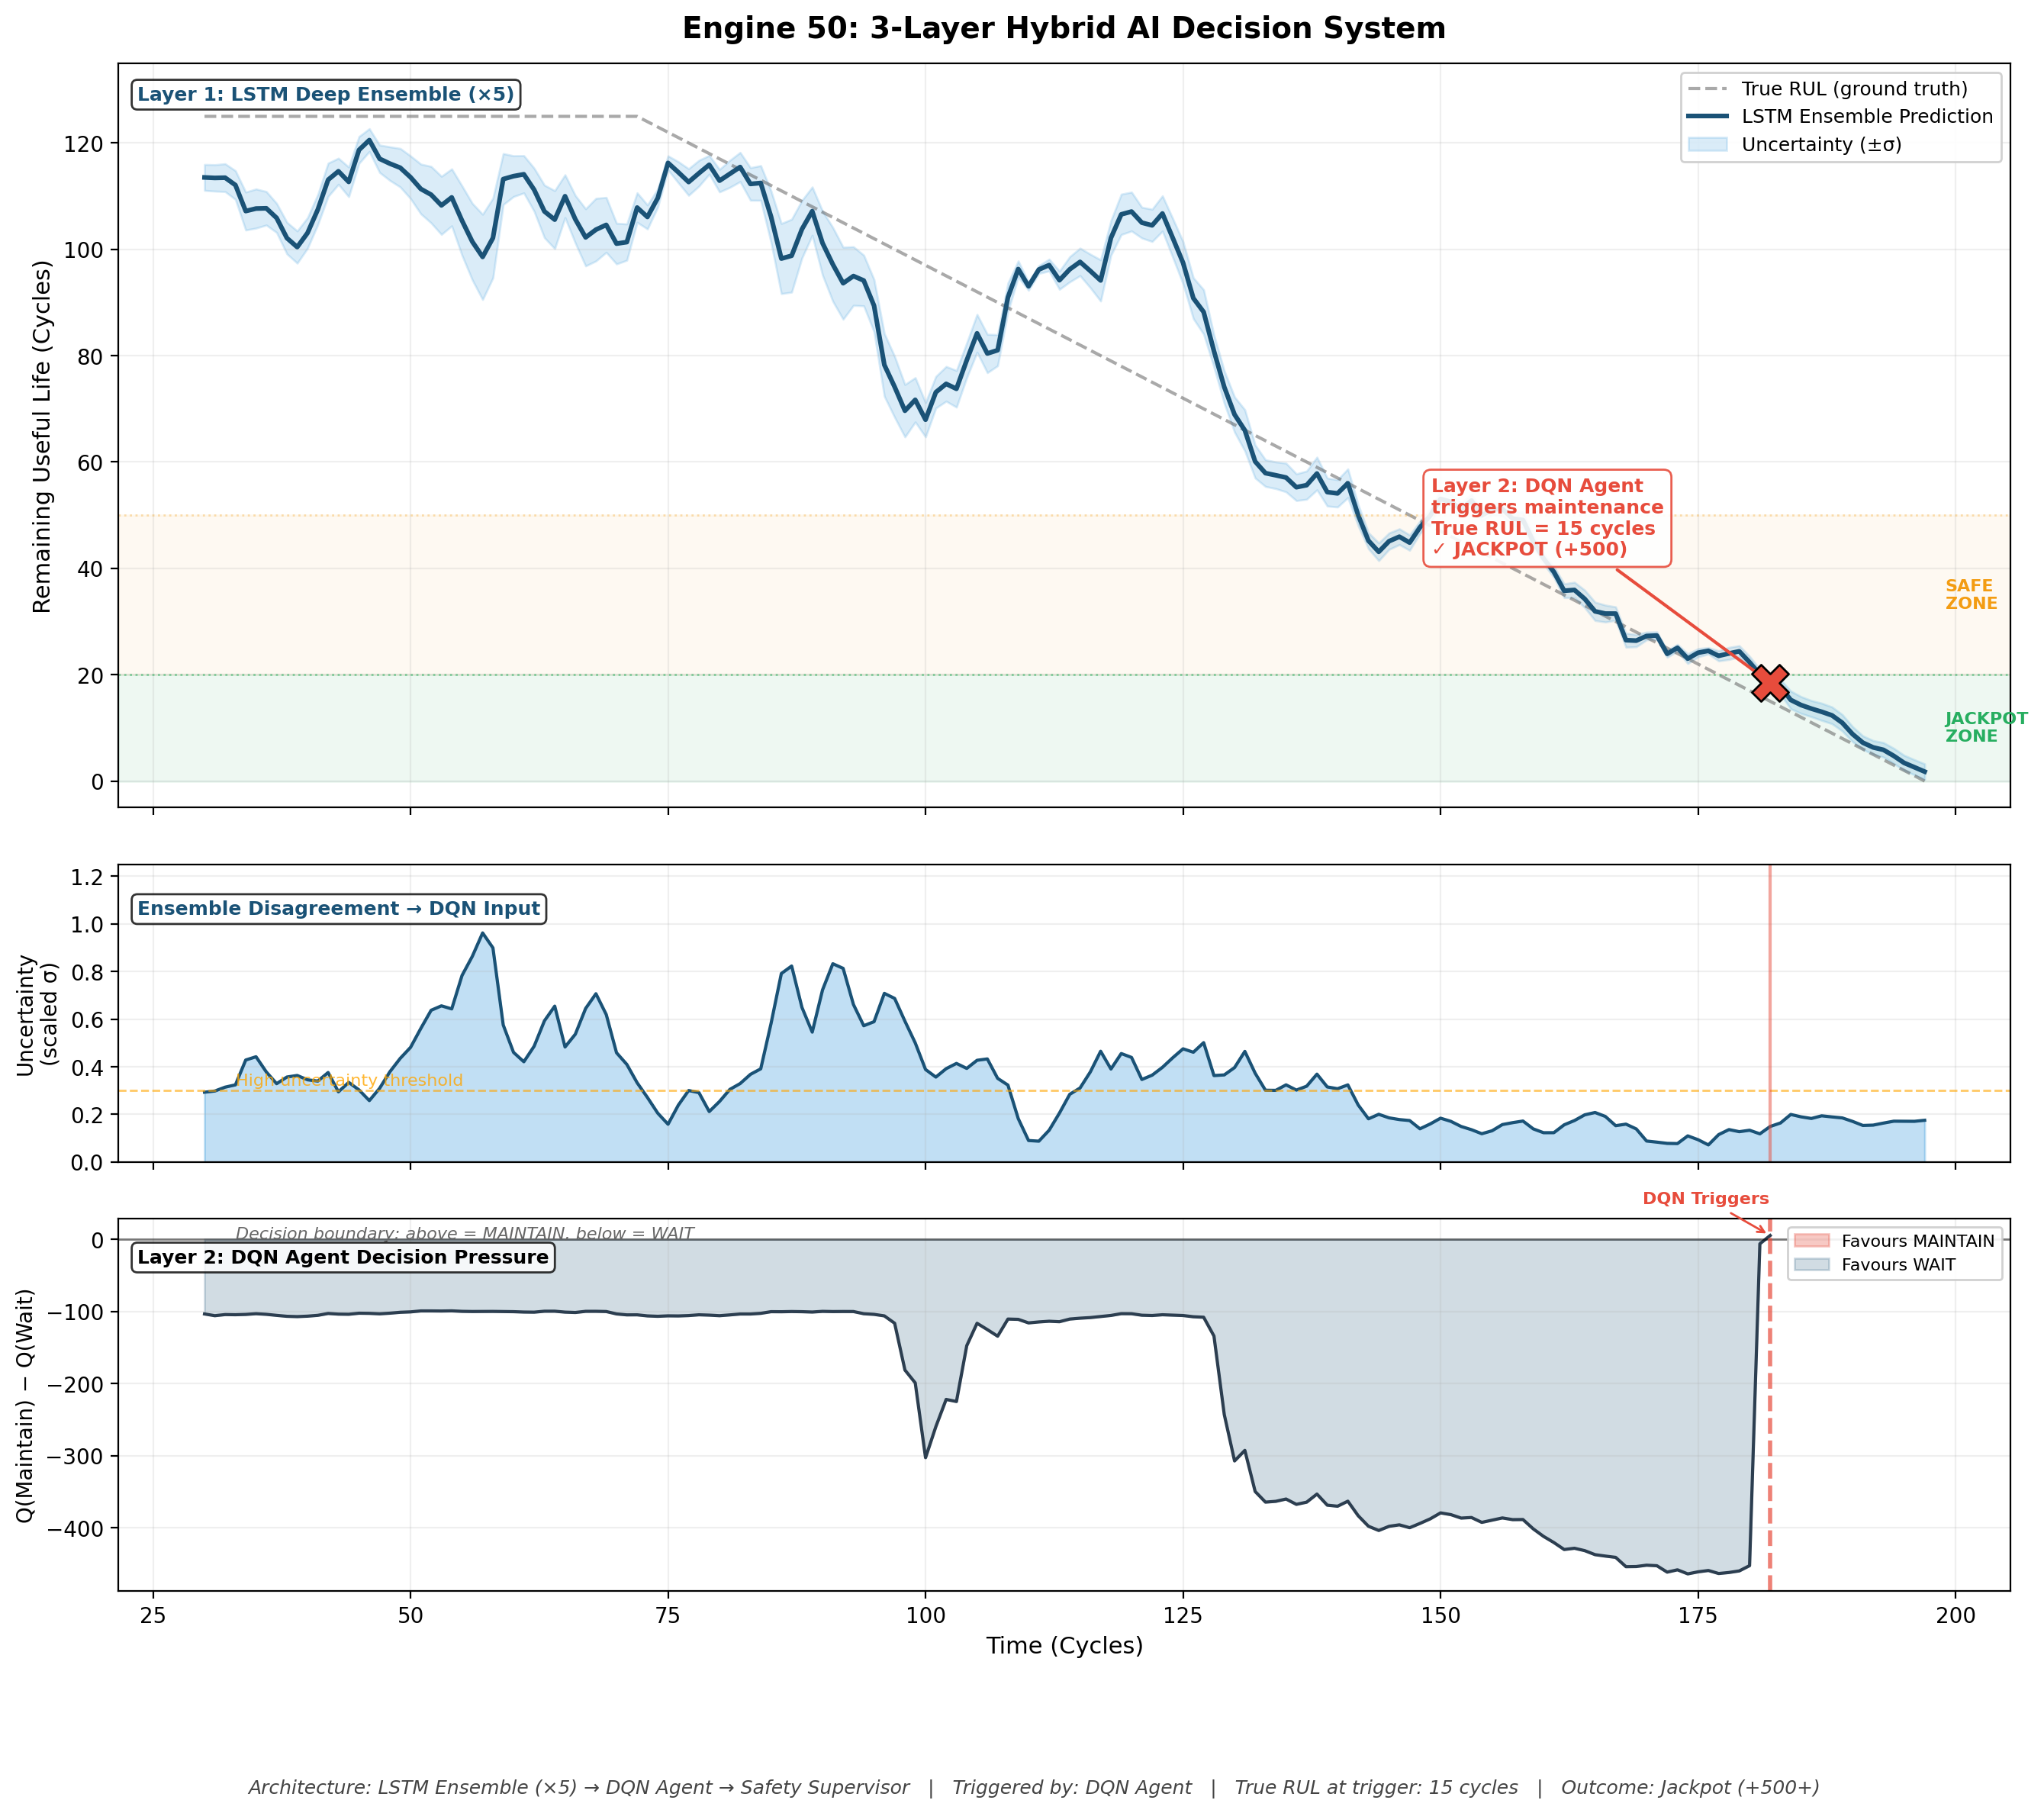
\includegraphics[width=0.95\textwidth]{final_engine_50_timeline.png}
\caption{Three-panel engine lifecycle timeline for Engine~50, showing: (top) ensemble RUL prediction with uncertainty band, (middle) scaled ensemble disagreement over time, and (bottom) DQN Q-value decision pressure. The vertical line indicates the cycle at which the agent triggered maintenance.}
\label{fig:engine_timeline}
\end{figure}

\subsection{Ablation Study Design}

The experimental evaluation was structured as a systematic ablation study comprising three experiments (Table~\ref{tab:ablation}), each designed to isolate the contribution of a specific system layer.


\begin{table}[h]
\centering
\caption{Ablation study design: three experiments isolating different system layers.}
\label{tab:ablation}
\renewcommand{\arraystretch}{1.3}
\begin{tabular}{>{\raggedright\arraybackslash}p{2.5cm} >{\raggedright\arraybackslash}p{3.5cm} >{\raggedright\arraybackslash}p{7cm}}
\toprule
\textbf{Experiment} & \textbf{Configuration} & \textbf{Research Question} \\
\midrule
Exp.~1: Layer~2 only & DQN agents without safety supervisor & Does uncertainty awareness improve the agent's autonomous decision-making under noise? \\
\addlinespace
Exp.~2: Full system & DQN agents with safety supervisor & Under the full three-layer system, does the UA agent still demonstrate superior behaviour, or does the safety net equalise performance? \\
\addlinespace
Exp.~3: Autonomy analysis & Delta between Exp.~2 and Exp.~1 & How much does each agent rely on the safety supervisor? Is the UA agent more autonomous? \\
\bottomrule
\end{tabular}
\end{table}


Each experiment evaluated both the uncertainty-aware (UA) agent and the blind agent across eight noise levels (0.000, 0.025, 0.050, 0.075, 0.100, 0.125, 0.150, 0.175) with 500 episodes per condition, yielding 4,000 episodes per agent per experiment and 24,000 episodes in total across all three experiments. Statistical comparison at each noise level used Welch's t-test ($\alpha = 0.05$) for significance and Cohen's d for effect size, following the conventions of \citet{cohen1988statistical}: $|d| < 0.2$ (negligible), $0.2 \leq |d| < 0.5$ (small), $0.5 \leq |d| < 0.8$ (medium), and $|d| \geq 0.8$ (large).

\section{Conclusions}

This chapter established a complete specification: twelve functional and six non-functional requirements, traced to the project objectives, with the system architecture separating prediction, decision-making, and safety into independently testable modules. Two design decisions merit emphasis: the symmetric $\pm 500$ crash/jackpot rewards that prevent risk-neutral behaviour, and the two-tier safety supervisor that interacts asymmetrically with the two agent types. The implementation is presented in Chapter~4.



\chapter{Implementation}

This chapter presents the implementation of the three-layer framework designed in Chapter~3, following the system's build order: data pipeline, LSTM ensemble, RL environment and agent, safety supervisor, and dashboard. Extended implementation details, engineering challenges, and testing documentation are provided in Appendix~\ref{app:impl_details} and Appendix~\ref{app:testing}.

\section{Code Repository Outline}

The codebase was developed from scratch in Python~3.9 with no starter code or templates. The repository uses a \texttt{src/} package for reusable modules and top-level scripts for training, evaluation, and experimentation.


\begin{table}[htbp]
\centering
\caption{Repository structure and purpose of each file.}
\label{tab:repo}
\renewcommand{\arraystretch}{1.3}
\setlength{\tabcolsep}{5pt}
\small
\begin{tabularx}{\textwidth}{>{\raggedright\arraybackslash}p{0.38\textwidth} >{\raggedright\arraybackslash}X}
\toprule
\textbf{File / Directory} & \textbf{Purpose} \\
\midrule
\path{src/config.py} & Centralised configuration for all hyperparameters (FR1--FR7, NF3). \\
\path{src/preprocessing.py} & Data loading, RUL calculation, normalisation, and sliding-window generation (FR1). \\
\path{src/lstm_model.py} & LSTM network architecture definition (FR2). \\
\path{src/gym_env.py} & Gymnasium environment, blind ablation variant, and safety supervisor (FR3, FR5, FR6). \\
\path{main_train_ensemble.py} & LSTM ensemble training with bootstrap sampling (FR2). \\
\path{main_train_rl.py} & DQN agent training with noise augmentation (FR4). \\
\path{main_experiment_final.py} & Three-experiment ablation study with statistical analysis (FR7). \\
\path{main_experiment_threshold.py} & Threshold baseline comparison (FR9). \\
\path{main_cost_analysis.py} & Fleet-level financial projection (FR8). \\
\path{main_evaluate_ensemble.py} & LSTM ensemble evaluation and diagnostic plots (FR10). \\
\path{main_visualize.py} & Engine lifecycle timeline visualisation (FR10). \\
\path{main_experiment_ppo.py} & PPO vs DQN algorithm comparison (Appendix~B.4). \\
\path{dashboard.py} & Streamlit interactive demonstration (FR11, FR12). \\
\path{test_system.py} & Automated \texttt{pytest} test suite (29 cases). \\
\path{data/} & NASA C-MAPSS dataset files (FD001, FD002). \\
\path{models/} & Trained model weights and scaler artefacts. \\
\bottomrule
\end{tabularx}
\end{table}


Third-party libraries comprised PyTorch \citep{paszke2019pytorch}, Stable-Baselines3 \citep{raffin2021stable}, Gymnasium \citep{brockman2016openai}, scikit-learn \citep{pedregosa2011scikit}, and Streamlit with Plotly. All components except the DQN training loop were implemented from scratch. Table~\ref{tab:repo} maps each file to its functional requirement.

Figure~\ref{fig:component_diagram} presents the end-to-end inference and decision pipeline, showing how raw sensor data is transformed into a maintenance action through the three architectural layers. The diagram traces the uncertainty signal ($\sigma$) from its origin in ensemble disagreement through the observation vector, reward shaping, and safety supervisor, highlighting the four distinct pathways through which uncertainty influences the final decision.

\begin{figure}[htbp]
\centering
\resizebox{\textwidth}{!}{%
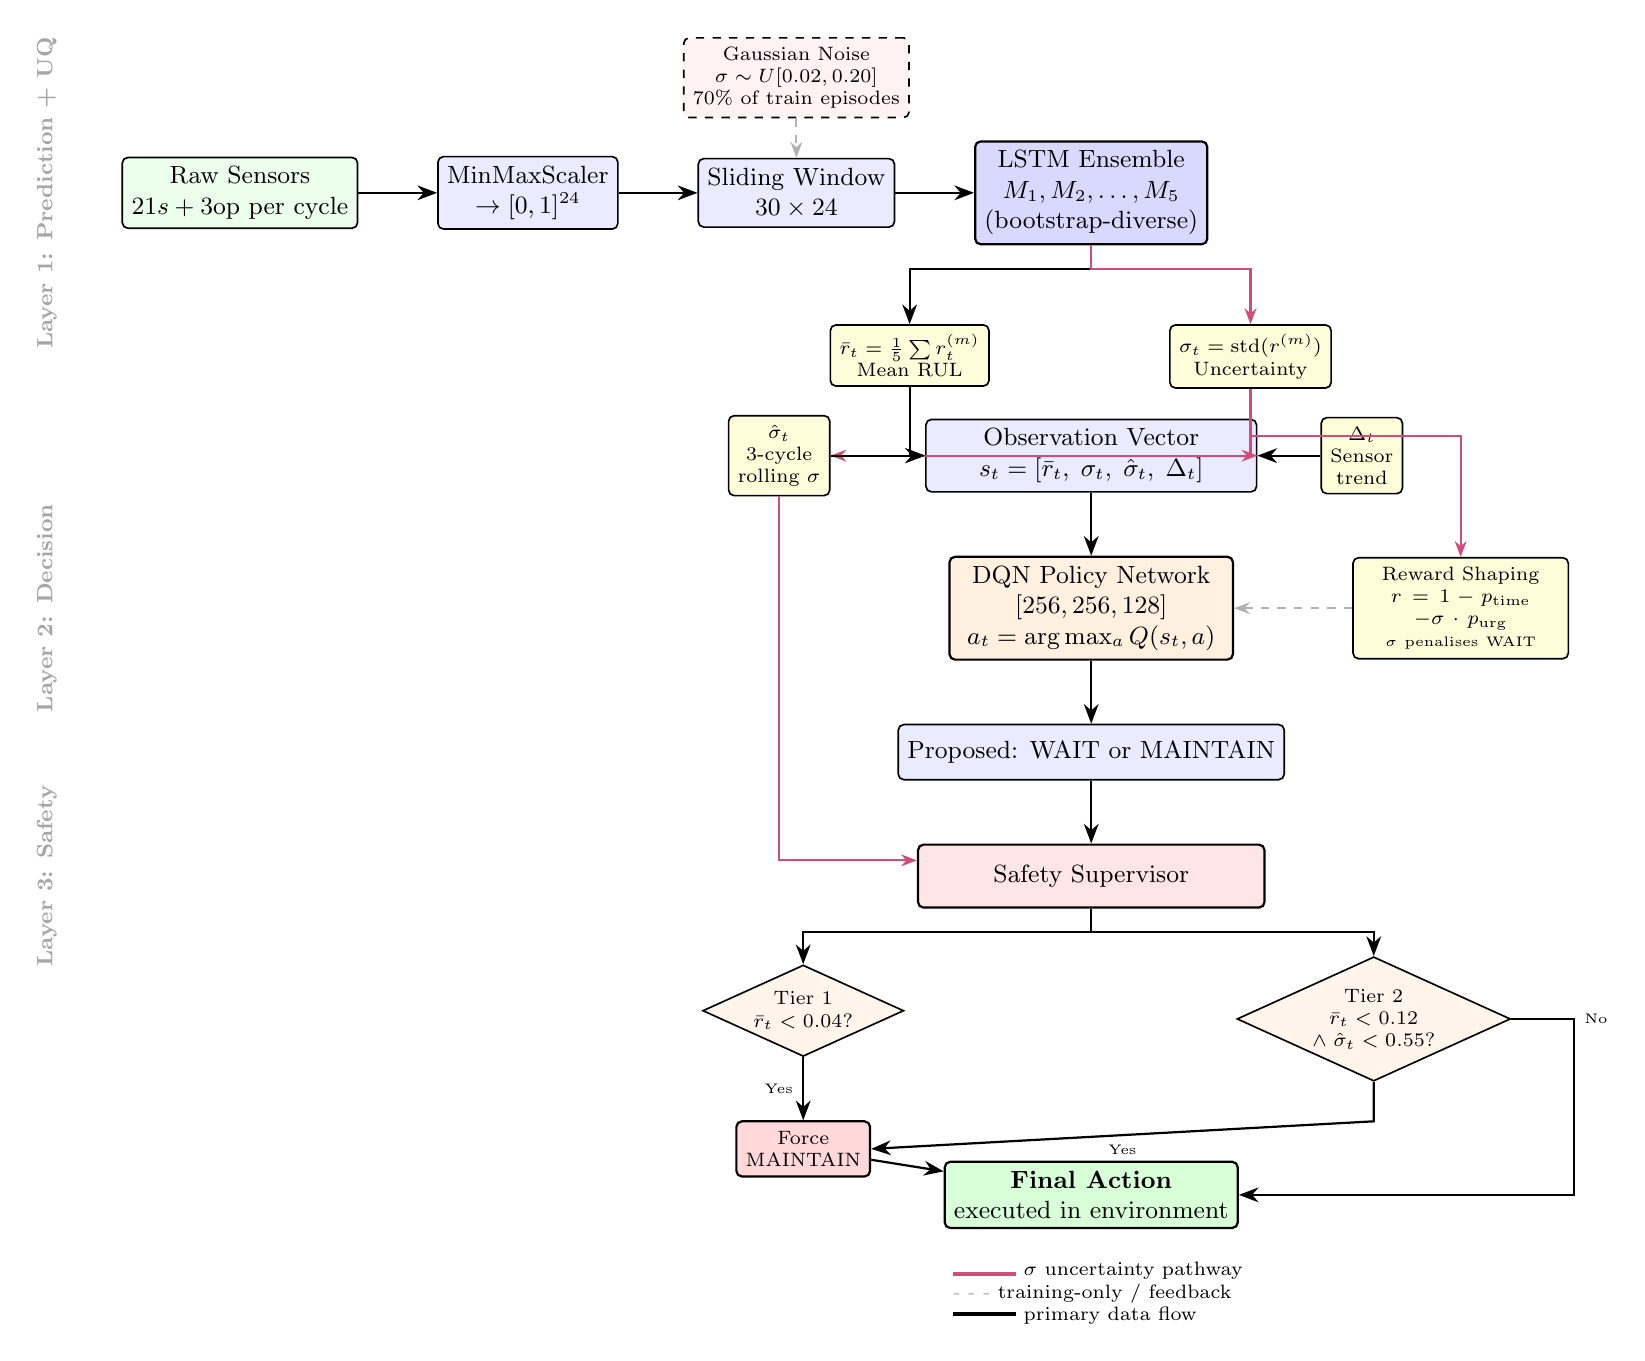
\begin{tikzpicture}[
  node distance=6mm and 8mm,
  every node/.style={font=\small},
  % Styles
  data/.style={rectangle, draw, rounded corners=2pt, minimum height=0.7cm, align=center, fill=green!8, line width=0.6pt},
  proc/.style={rectangle, draw, rounded corners=2pt, minimum height=0.7cm, align=center, fill=blue!8, line width=0.6pt},
  model/.style={rectangle, draw, rounded corners=2pt, minimum height=0.8cm, align=center, fill=blue!15, line width=0.8pt},
  agent/.style={rectangle, draw, rounded corners=2pt, minimum height=0.8cm, align=center, fill=orange!12, line width=0.8pt},
  safety/.style={rectangle, draw, rounded corners=2pt, minimum height=0.8cm, align=center, fill=red!10, line width=0.8pt},
  decision/.style={diamond, draw, aspect=2.2, align=center, fill=orange!8, line width=0.6pt, inner sep=1pt, font=\scriptsize},
  signal/.style={rectangle, draw, rounded corners=2pt, minimum height=0.6cm, align=center, fill=yellow!15, line width=0.6pt, font=\scriptsize},
  outcome/.style={rectangle, draw, rounded corners=2pt, minimum height=0.7cm, align=center, fill=green!15, line width=0.8pt},
  noise/.style={rectangle, draw, dashed, rounded corners=2pt, minimum height=0.6cm, align=center, fill=red!5, line width=0.6pt, font=\scriptsize},
  arr/.style={-{Stealth[length=2.5mm]}, thick},
  sigarr/.style={-{Stealth[length=2mm]}, thick, color=purple!70},
  dasharr/.style={-{Stealth[length=2mm]}, dashed, thick, color=gray!60},
  layerlabel/.style={font=\bfseries\footnotesize, text=gray!70, rotate=90, anchor=south},
]

  % ── LAYER 1: LSTM ENSEMBLE ────────────────────────────────
  % Input
  \node[data] (raw) {Raw Sensors\\$21s + 3\text{op}$ per cycle};
  \node[proc, right=10mm of raw] (preproc) {MinMaxScaler\\$\to [0,1]^{24}$};
  \node[proc, right=10mm of preproc] (window) {Sliding Window\\$30 \times 24$};

  % Noise injection (training only)
  \node[noise, above=5mm of window] (noise) {Gaussian Noise\\$\sigma \sim U[0.02, 0.20]$\\70\% of train episodes};

  % Ensemble
  \node[model, right=10mm of window, minimum width=2.8cm] (ens) {LSTM Ensemble\\$M_1, M_2, \ldots, M_5$\\(bootstrap-diverse)};

  % Ensemble outputs
  \node[signal, below left=10mm and -2mm of ens] (mu) {$\bar{r}_t = \frac{1}{5}\sum r_t^{(m)}$\\Mean RUL};
  \node[signal, below right=10mm and -5mm of ens] (sigma) {$\sigma_t = \text{std}(r^{(m)})$\\Uncertainty};

  % ── LAYER 2: DQN AGENT ────────────────────────────────────
  % Observation construction
  \node[proc, below=22mm of ens, minimum width=4.2cm] (obs) {Observation Vector\\$s_t = [\bar{r}_t,\; \sigma_t,\; \hat{\sigma}_t,\; \Delta_t]$};

  % Derived signals feeding into obs
  \node[signal, left=12mm of obs] (rolling) {$\hat{\sigma}_t$\\3-cycle\\rolling $\sigma$};
  \node[signal, right=8mm of obs] (trend) {$\Delta_t$\\Sensor\\trend};

  % DQN
  \node[agent, below=8mm of obs, minimum width=3.6cm] (dqn) {DQN Policy Network\\$[256, 256, 128]$\\$a_t = \arg\max_a Q(s_t, a)$};

  % Proposed action
  \node[proc, below=8mm of dqn] (proposed) {Proposed: WAIT or MAINTAIN};

  % Reward shaping (feedback)
  \node[signal, right=15mm of dqn, text width=2.5cm] (reward) {Reward Shaping\\$r = 1 - p_{\text{time}}$\\$- \sigma \cdot p_{\text{urg}}$\\{\tiny $\sigma$ penalises WAIT}};

  % ── LAYER 3: SAFETY SUPERVISOR ────────────────────────────
  \node[safety, below=8mm of proposed, minimum width=4.4cm] (super) {Safety Supervisor};

  % Two tiers
  \node[decision, below left=10mm and 8mm of super] (t1) {Tier 1\\$\bar{r}_t < 0.04$?};
  \node[decision, below right=10mm and 5mm of super] (t2) {Tier 2\\$\bar{r}_t < 0.12$\\$\wedge\; \hat{\sigma}_t < 0.55$?};

  % Final action
  \node[outcome, below=32mm of super] (final) {\textbf{Final Action}\\executed in environment};

  % Override label
  \node[outcome, below=8mm of t1, fill=red!15, minimum width=1.6cm, font=\scriptsize] (force) {Force\\MAINTAIN};

  % ── ARROWS ────────────────────────────────────────────────
  % Layer 1 flow
  \draw[arr] (raw) -- (preproc);
  \draw[arr] (preproc) -- (window);
  \draw[arr] (window) -- (ens);
  \draw[dasharr] (noise) -- (window);

  % Ensemble to outputs
  \draw[arr] (ens.south) -- ++(0,-0.3) -| (mu.north);
  \draw[sigarr] (ens.south) -- ++(0,-0.3) -| (sigma.north);

  % Outputs to observation
  \draw[arr] (mu.south) |- (obs.west);
  \draw[sigarr] (sigma.south) |- (obs.east);
  \draw[sigarr] (sigma.south) |- (rolling.east);
  \draw[arr] (rolling) -- (obs);
  \draw[arr] (trend) -- (obs);

  % Observation to DQN
  \draw[arr] (obs) -- (dqn);
  \draw[arr] (dqn) -- (proposed);

  % Reward feedback
  \draw[dasharr] (reward) -- (dqn);
  \draw[sigarr] (sigma.south) -- ++(0,-0.6) -| (reward.north);

  % DQN to supervisor
  \draw[arr] (proposed) -- (super);

  % Supervisor internals
  \draw[arr] (super.south) -- ++(0,-0.3) -| (t1.north);
  \draw[arr] (super.south) -- ++(0,-0.3) -| (t2.north);

  % Tier outcomes
  \draw[arr] (t1) -- node[left, font=\tiny] {Yes} (force);
  \draw[arr] (t2.south) -- ++(0,-0.5) -- node[below, font=\tiny] {Yes} (force.east);
  \draw[arr] (force) -- (final);

  % Pass-through
  \draw[arr] (t2.east) -- ++(0.8,0) node[right, font=\tiny] {No} |- (final.east);

  % Sigma to supervisor (confidence check)
  \draw[sigarr] (rolling.south) |- ([yshift=2mm]super.west);

  % ── LAYER LABELS ──────────────────────────────────────────
  \node[layerlabel] at ([xshift=-7mm]raw.west |- ens) {Layer 1: Prediction + UQ};
  \node[layerlabel] at ([xshift=-7mm]raw.west |- dqn) {Layer 2: Decision};
  \node[layerlabel] at ([xshift=-7mm]raw.west |- super) {Layer 3: Safety};

  % ── LEGEND ────────────────────────────────────────────────
  \node[font=\scriptsize, anchor=north west, text width=4cm] at ([yshift=-3mm]final.south west) {
    \textcolor{purple!70}{\rule{8mm}{1.5pt}} $\sigma$ uncertainty pathway\\
    \textcolor{gray!60}{- - -} training-only / feedback\\
    \rule[0.5ex]{8mm}{1.5pt} primary data flow
  };

\end{tikzpicture}%
}% end resizebox
\caption{End-to-end inference and decision pipeline showing all three architectural layers. The purple arrows trace the uncertainty signal ($\sigma$) from its origin in ensemble disagreement through four distinct pathways: (1)~direct observation input, (2)~rolling average for smoothed trend, (3)~reward shaping penalty for waiting under high uncertainty, and (4)~confidence gate for the safety supervisor's Tier~2 override. The dashed path from the noise injection block is active only during training.}
\label{fig:component_diagram}
\end{figure}

\section{Data Pipeline}

The data pipeline (FR1) loaded and merged C-MAPSS FD001 (100 engines, single operating condition) and FD002 (260 engines, six operating conditions), yielding 360 run-to-failure trajectories. FD002 unit IDs were offset by 100 to prevent cross-subset collisions. RUL was capped at 125 cycles following \citet{heimes2008recurrent}, all 24 features were scaled to $[0, 1]$ using MinMaxScaler \citep{pedregosa2011scikit}, and sliding windows of 30 cycles produced approximately 46,000 training sequences. Full pipeline details are provided in Appendix~\ref{app:impl_details}.

\section{LSTM Ensemble Training}

Five LSTM networks (FR2) were trained on 80\% bootstrap samples of the training data (seed = 42 + $i \times 17$), following the diversity strategy of \citet{fort2019deep}. Each model comprised a two-layer LSTM (hidden dimension 100, dropout 0.2) followed by a linear output layer. Training used Adam \citep{kingma2014adam} with learning rate $5 \times 10^{-4}$, ReduceLROnPlateau scheduling, early stopping (patience 15), and gradient clipping at 1.0. Models converged within 40--60 epochs, achieving validation RMSE of 12--15 cycles. At inference time, the ensemble mean served as the point estimate and the standard deviation quantified uncertainty \citep{lakshminarayanan2017simple}. Figure~\ref{fig:uncertainty_error} confirms that ensemble disagreement correlates with prediction error, validating the uncertainty signal \citep{ovadia2019can}. The full training procedure and hyperparameters are documented in Appendix~\ref{app:hyperparams}.

\begin{figure}[h]
\centering
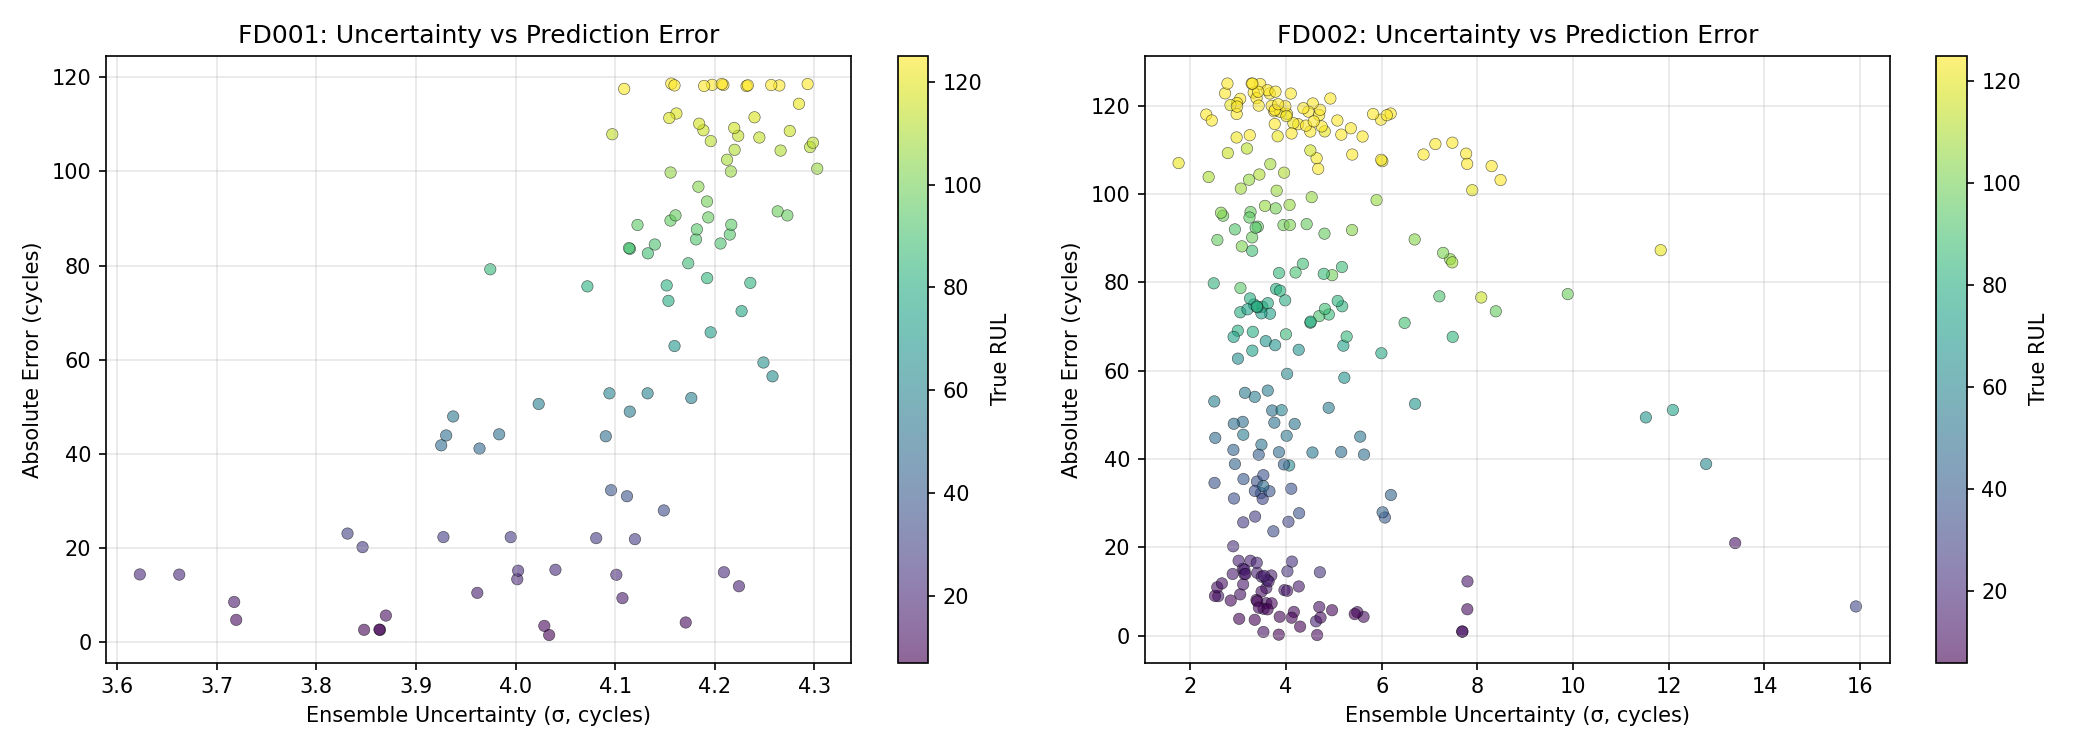
\includegraphics[width=0.85\textwidth]{uncertainty_vs_error.png}
\caption{Ensemble uncertainty (standard deviation) plotted against absolute prediction error on the C-MAPSS test set. The positive correlation confirms that ensemble disagreement is a well-calibrated indicator of prediction reliability \citep{lakshminarayanan2017simple}.}
\label{fig:uncertainty_error}
\end{figure}

\section{Gymnasium Reinforcement Learning Environment}

The \texttt{PdMEnvironment} class (FR3) extended \texttt{gymnasium.Env} \citep{brockman2016openai} and translated the MDP formulation from Section~3.5.2 into executable code. At each step, a 30-cycle sensor window was passed through the ensemble, and the resulting mean, scaled standard deviation (UNCERTAINTY\_SCALE = 15), rolling uncertainty average, and sensor trend formed the four-dimensional observation vector.


\textbf{Noise augmentation.} Per-episode noise injection \citep{tobin2017domain, wang2020remaining} was applied with probability 0.7, sampling noise standard deviation uniformly from $[0.02, 0.20]$. This variable-noise design exposed the agent to a continuous spectrum of degradation intensities during training.


\textbf{End-of-life training bias.} To counter the class imbalance (87\% of random starts fall in the healthy phase), 60\% of training episodes were initialised within the last 50 cycles, ensuring sufficient exposure to critical decision points \citep{lin1992self}.


\textbf{Reward implementation.} The reward function followed Table~\ref{tab:reward}, with additional time-pressure decay below 25 cycles, an uncertainty urgency penalty for waiting under high uncertainty in the buffer zone, and a proactive maintenance bonus of $+30$ for acting under uncertainty near end of life.


\textbf{Blind ablation.} The \texttt{BlindPdMEnvironment} subclass (FR5) zeroed both uncertainty dimensions ($\sigma_t = 0$, $\hat{\sigma}_t = 0$) while preserving state dimensionality, ensuring any performance difference was attributable solely to the uncertainty signal.

\section{DQN Agent Training}

The DQN agent (FR4) used a $[256, 256, 128]$ fully connected Q-network \citep{mnih2015human}, trained for 1.5 million timesteps via Stable-Baselines3 \citep{raffin2021stable} with a 150,000-transition replay buffer, $\gamma = 0.99$, and $\epsilon$-greedy exploration decaying from 1.0 to 0.03 over 40\% of training. The noise augmentation and end-of-life bias exposed the agent to clean, moderate, and heavy noise regimes, teaching it to adapt its policy to the current uncertainty level rather than memorise a fixed mapping. The blind control agent was trained identically but on the \texttt{BlindPdMEnvironment}, which zeroed the uncertainty dimensions. Full hyperparameters are listed in Appendix~\ref{app:hyperparams}.

\section{Safety Supervisor}

The safety supervisor implemented FR6 as a pure Python function that accepted the DQN agent's proposed action and the current observation vector and returned a possibly modified action. The implementation was deliberately kept outside any learned component to provide deterministic and auditable intervention logic, following the shielding principle formalised by \citet{alshiekh2018safe} and the defence-in-depth requirement of aerospace safety standards \citep{do178c}.


\textbf{Two-tier logic.} As specified in Section~3.5.3, the function implemented two override conditions evaluated in priority order. Tier~1 (hard critical) fired unconditionally when the ensemble mean prediction fell below 0.04 (approximately 5 cycles remaining), providing a deterministic last-resort intervention. Tier~2 (uncertainty-aware) fired when the prediction fell below 0.12 (approximately 15 cycles) \emph{and} the rolling uncertainty was below 0.55, ensuring that the override only engaged when the ensemble was confident in its low-RUL assessment. If neither condition was met, the agent's original action passed through unmodified.


\textbf{Interaction with the two agent types.} The design created an asymmetry central to evaluation. Because the blind agent reports rolling uncertainty of zero, it almost always satisfies the confidence condition and is overridden more often, including on some noise-driven low predictions. The UA agent reports true disagreement, so confidence-gated overrides are more selective, preserving autonomy while retaining hard-critical protection.

\section{Interactive Dashboard}

The Streamlit dashboard (FR11, FR12) provided a real-time demonstration of the full pipeline using the same trained models and data as the evaluation scripts. The sidebar offered toggles for agent type, safety supervisor, and noise intensity. Three live Plotly charts displayed the RUL prediction with uncertainty band, rolling uncertainty trend, and DQN Q-value decision pressure, updated cycle by cycle. Figure~\ref{fig:dashboard} presents the interface during a representative run.

\begin{figure}[h]
\centering
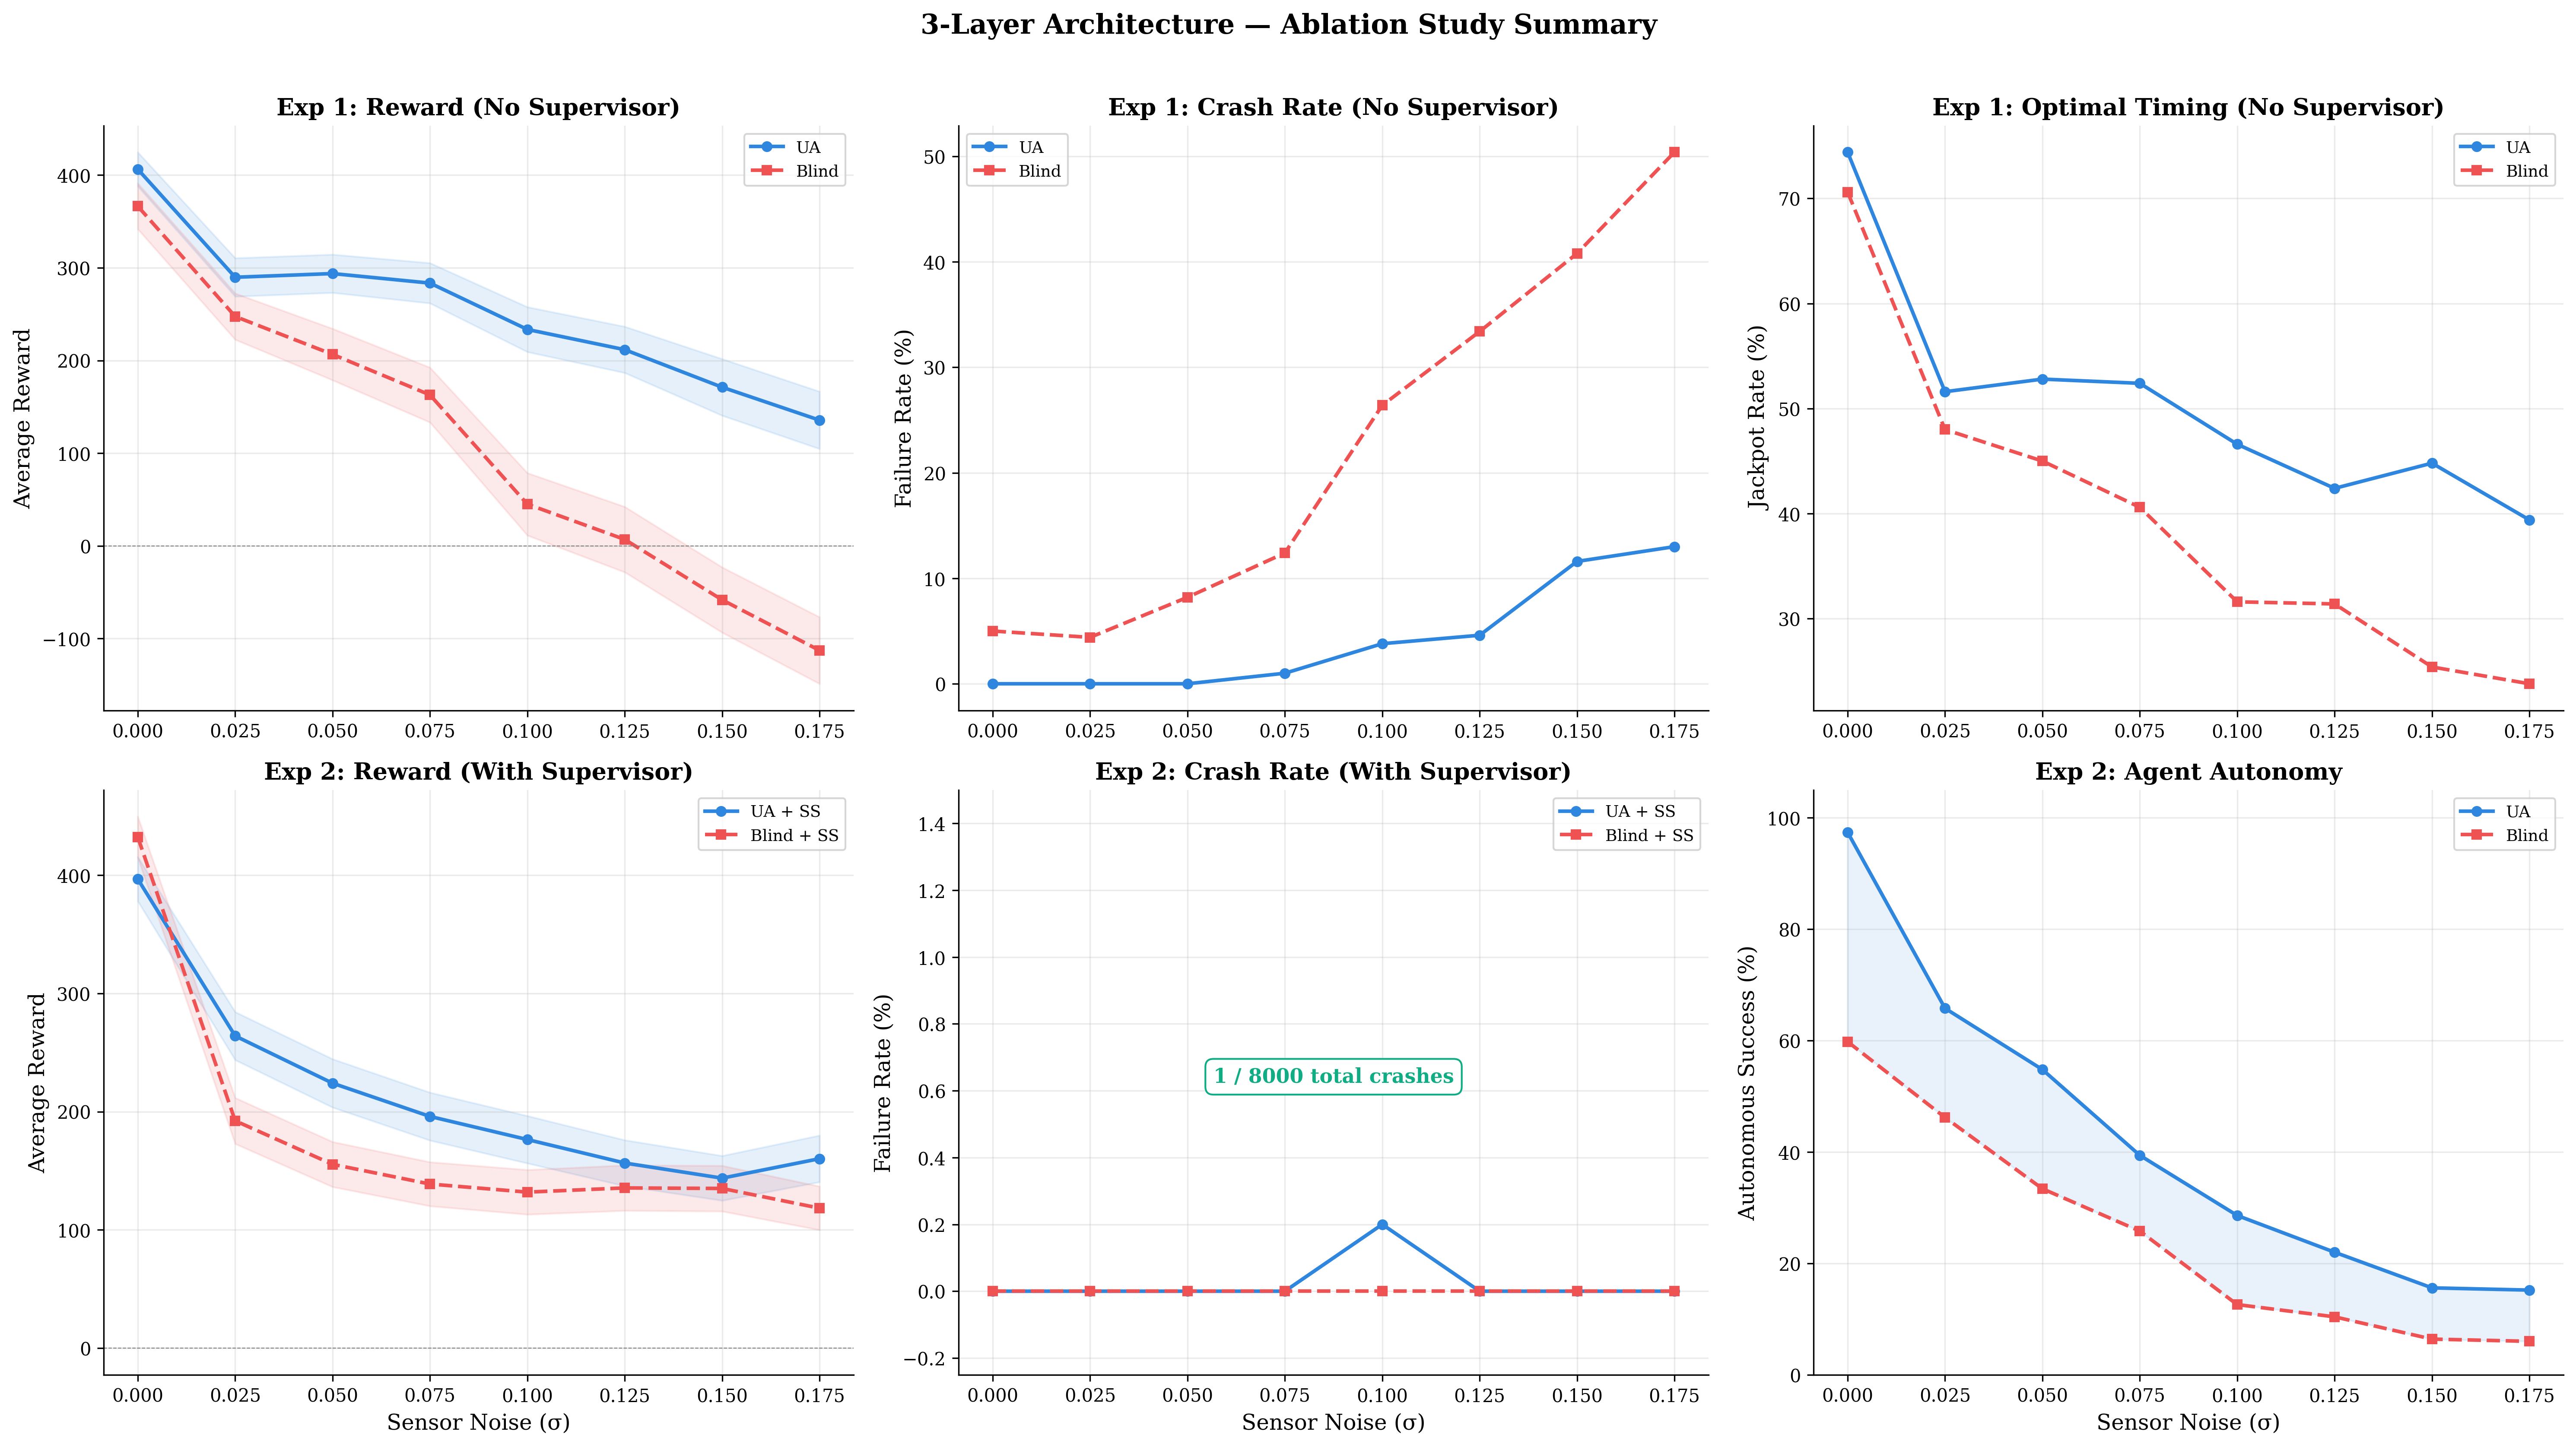
\includegraphics[width=0.95\textwidth]{report_summary_dashboard.png}
\caption{The Streamlit interactive dashboard during a simulation run, showing the three-panel visualisation (RUL prediction, uncertainty trend, and Q-value decision pressure), the status panel, and the sidebar controls for agent type, safety supervisor, and noise intensity.}
\label{fig:dashboard}
\end{figure}

\section{Implementation Challenges}

Three non-trivial challenges arose during development. First, end-of-life class imbalance caused early agents to learn a ``wait forever'' policy; this was resolved by biasing 60\% of episodes to start within the last 50 cycles. Second, the raw ensemble standard deviation range (0.01--0.10) was too narrow for the DQN; the UNCERTAINTY\_SCALE factor of 15 was calibrated to provide clear separation across noise regimes, directly informing the supervisor's confidence threshold of 0.55. Third, the initial crash penalty of $-100$ was insufficient (discounted present value of only $-20$ at 160 steps); increasing it to $-500$ made crash avoidance material from early degradation. Extended details are provided in Appendix~\ref{app:impl_details}.

\section{Testing}

Testing was conducted at three levels using an automated \texttt{pytest} suite (\texttt{test\_system.py}, 29 test cases, all passing). Unit tests verified individual module correctness (data pipeline, LSTM output shapes, environment API compliance); integration tests confirmed ensemble-environment interaction, agent loading, and safety supervisor override behaviour; and system-level validation ran the ablation study on a subset of conditions to verify statistical outputs and reproducibility. The full testing protocol and results are documented in Appendix~\ref{app:testing}.


Figures~\ref{fig:engine_134} and~\ref{fig:engine_200} show two contrasting lifecycle traces: a smooth degradation case and a noisier case that stresses uncertainty handling.

\begin{figure}[h]
\centering

\includegraphics[width=0.95\textwidth]{final_engine_134_timeline.png}
\caption{Three-panel engine lifecycle timeline for Engine~134, showing the ensemble RUL prediction with uncertainty band (top), scaled ensemble disagreement (middle), and DQN Q-value decision pressure (bottom). The smooth degradation profile allowed the agent to make a confident, timely maintenance decision.}
\label{fig:engine_134}
\end{figure}

\begin{figure}[h]
\centering
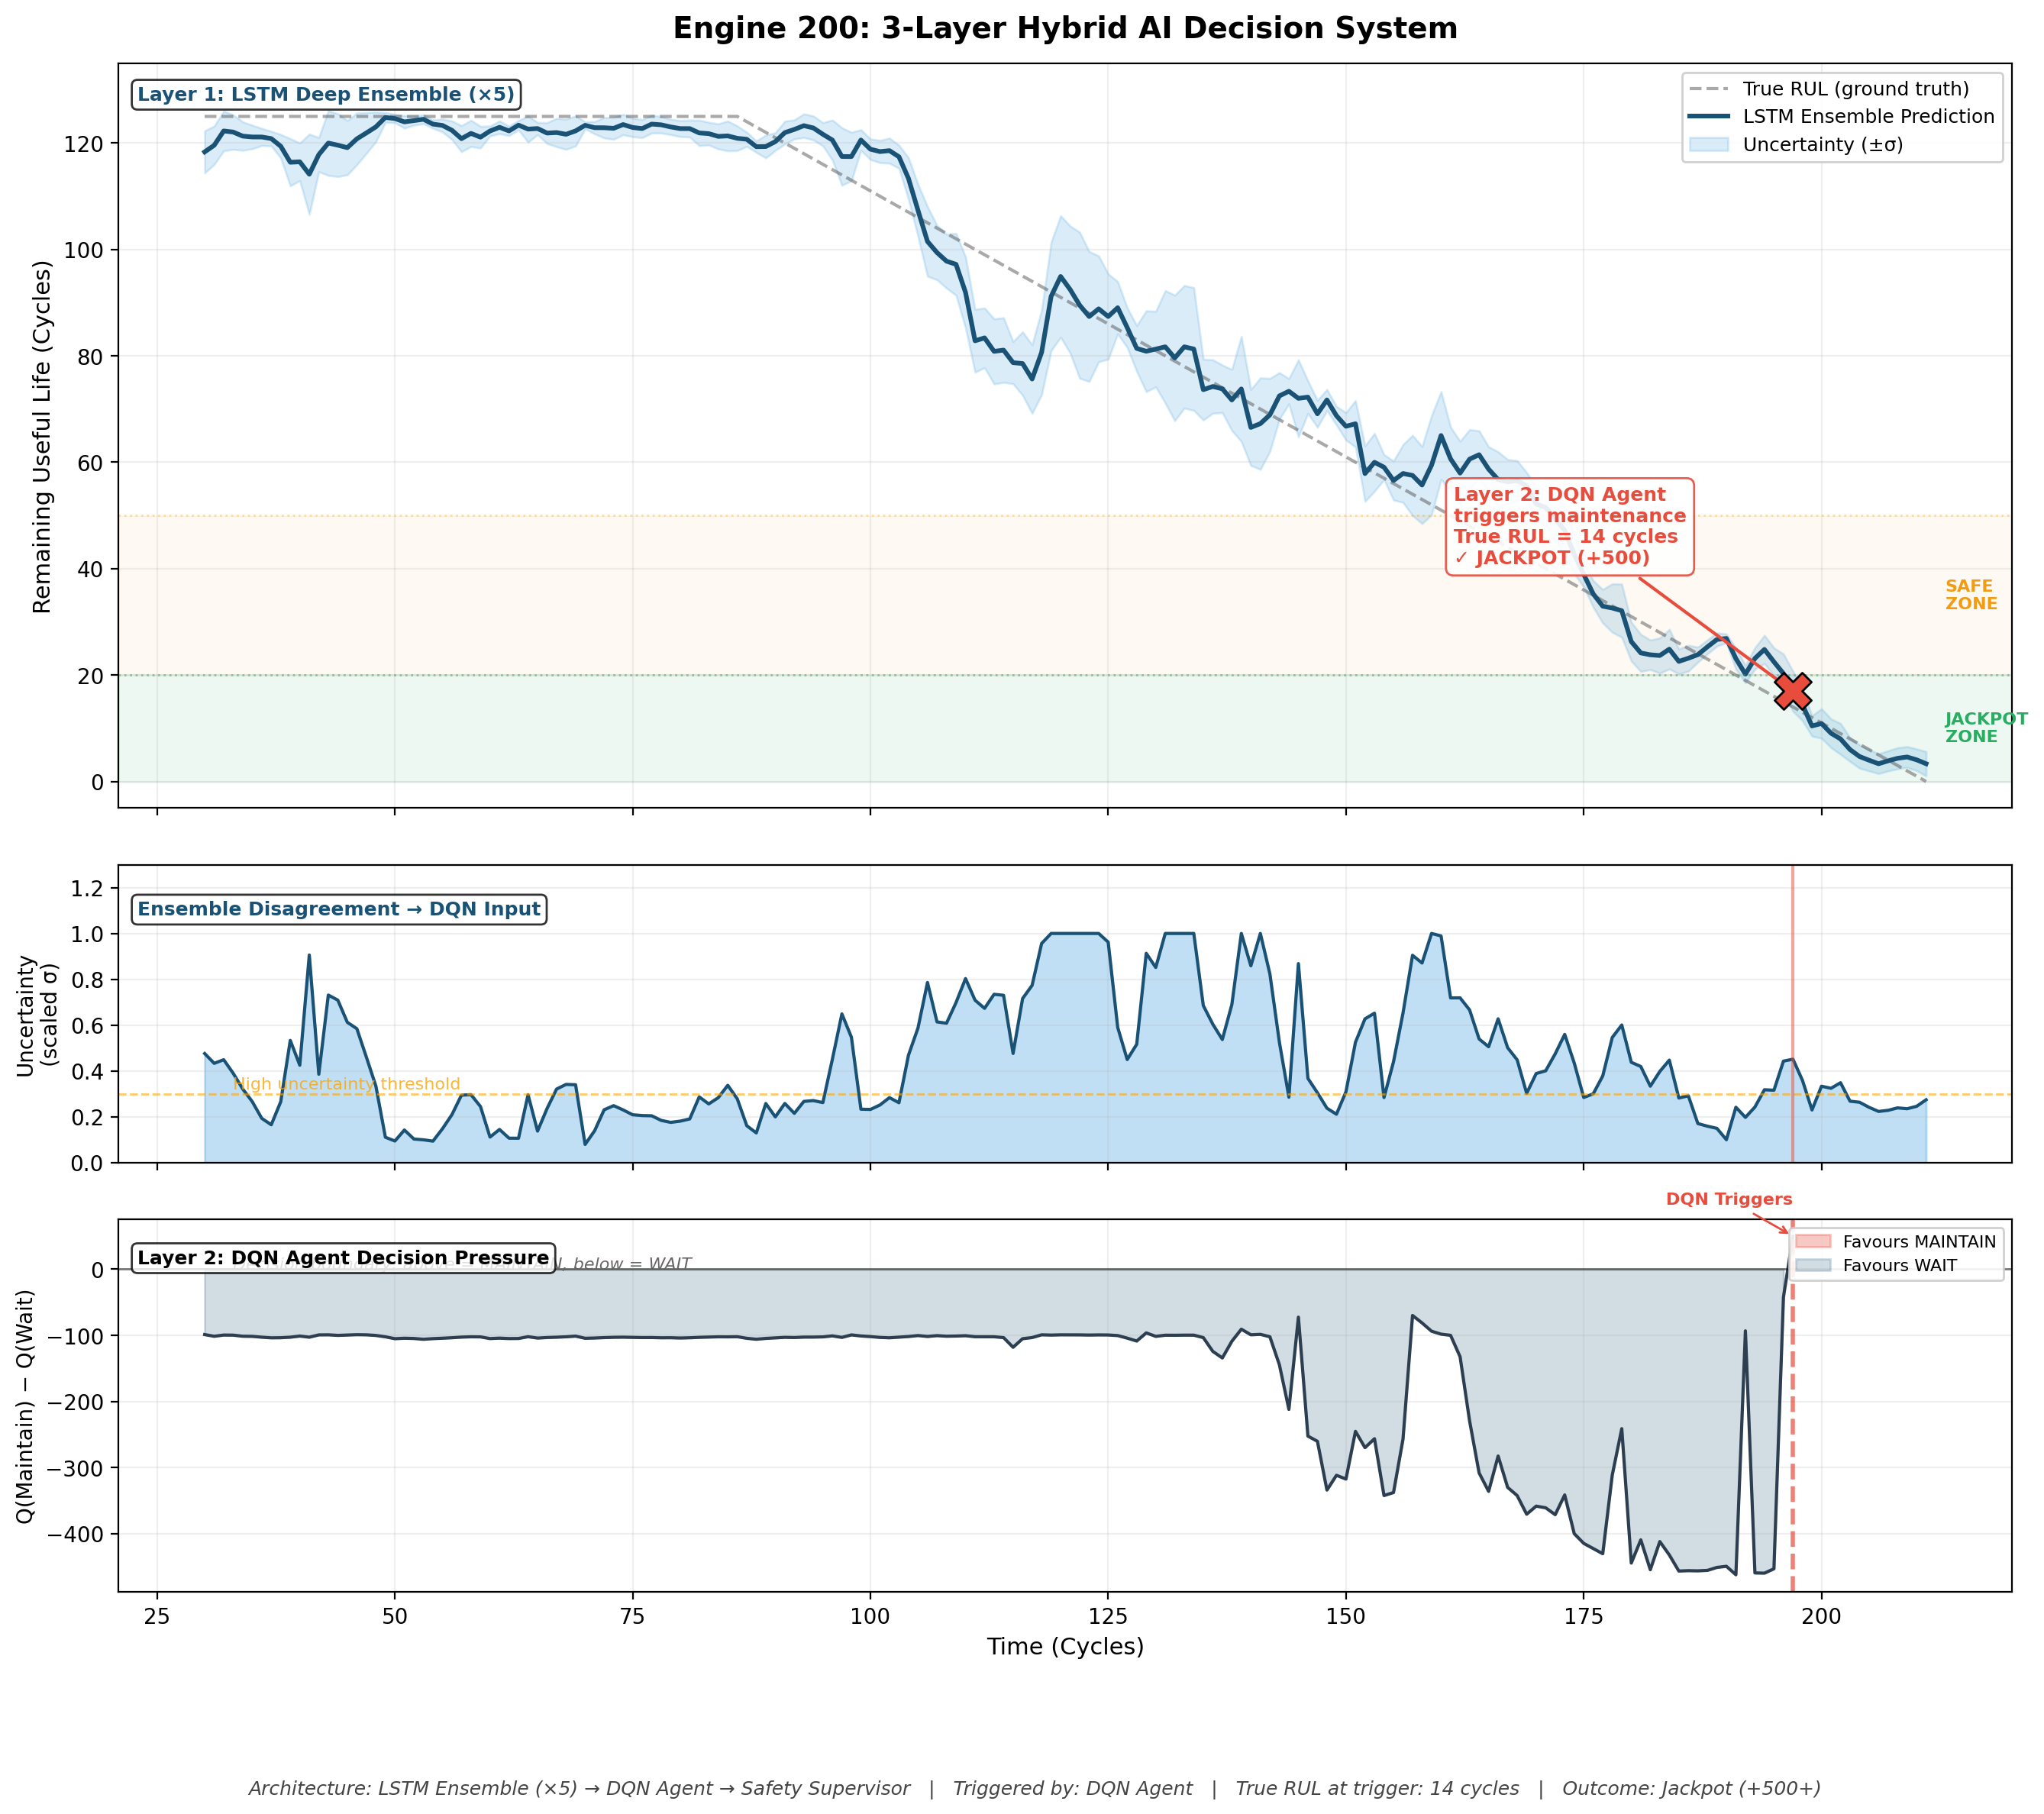
\includegraphics[width=0.95\textwidth]{final_engine_200_timeline.png}
\caption{Three-panel engine lifecycle timeline for Engine~200, demonstrating the system's behaviour under a noisier degradation trajectory. The elevated uncertainty in the middle panel shows the ensemble responding to ambiguous sensor data, while the agent adapts its decision timing accordingly.}
\label{fig:engine_200}
\end{figure}

\section{Conclusion}

All twelve functional requirements were implemented and verified. The data pipeline (FR1), LSTM ensemble (FR2), Gymnasium environment (FR3, FR5), DQN agent (FR4), safety supervisor (FR6), and Streamlit dashboard (FR11, FR12) operated as designed. Three engineering challenges required iterative resolution beyond the initial specification; testing at unit, integration, and system levels confirmed requirement satisfaction. The experimental results are presented in Chapter~5.




\chapter{Results and Evaluation}

This chapter presents the experimental results and evaluates the system against the project objectives (Section~1.2). Results are reported objectively first, followed by a critical assessment of achievement, limitations, and positioning within the literature.

\section{Results}

The experimental evaluation followed the ablation study design specified in Table~\ref{tab:ablation}, producing 24,000 episodes across three experiments, two agent types, and eight noise levels. All experiments used 500 episodes per condition with fixed random seeds for reproducibility (NF1). Statistical comparisons employed Welch's t-test ($\alpha = 0.05$) for significance and Cohen's d for effect size, following the conventions of \citet{cohen1988statistical}.

\subsection{Experiment 1: Layer 2 Isolation}

Experiment~1 evaluated the DQN agents without the safety supervisor to isolate the contribution of uncertainty awareness to the agent's autonomous decision-making. Table~\ref{tab:exp1_results} summarises the key metrics across all eight noise levels.


\begin{table}[h]
\centering
\small
\caption{Experiment~1 results: UA vs Blind agent without safety supervisor. Significance: * $p < 0.05$, ** $p < 0.01$, *** $p < 0.001$, ns = not significant.}
\label{tab:exp1_results}
\renewcommand{\arraystretch}{1.2}
\setlength{\tabcolsep}{4pt}
\resizebox{\textwidth}{!}{%
\begin{tabular}{>{\raggedright\arraybackslash}p{1.2cm} r r r r r r l l}
\toprule
\textbf{Noise} & \textbf{UA Mean} & \textbf{UA Fail\%} & \textbf{UA Jack\%} & \textbf{Blind Mean} & \textbf{Blind Fail\%} & \textbf{Blind Jack\%} & \textbf{Sig.} & \textbf{Cohen's d} \\
\midrule
0.000 & 406.4 & 0.0 & 74.4 & 366.4 & 5.0 & 70.6 & * & 0.16 \\
0.025 & 289.8 & 0.0 & 51.6 & 247.5 & 4.4 & 48.0 & * & 0.16 \\
0.050 & 293.8 & 0.0 & 52.8 & 206.6 & 8.2 & 45.0 & *** & 0.31 \\
0.075 & 283.5 & 1.0 & 52.4 & 162.8 & 12.4 & 40.6 & *** & 0.41 \\
0.100 & 233.5 & 3.8 & 46.6 & 45.0 & 26.4 & 31.6 & *** & 0.56 \\
0.125 & 211.6 & 4.6 & 42.4 & 6.9 & 33.4 & 31.4 & *** & 0.59 \\
0.150 & 171.1 & 11.6 & 44.8 & $-58.3$ & 40.8 & 25.4 & *** & 0.61 \\
0.175 & 135.6 & 13.0 & 39.4 & $-112.8$ & 50.4 & 23.8 & *** & 0.65 \\
\bottomrule
\end{tabular}
}
\end{table}


Three patterns are immediately visible. First, the UA agent maintained positive mean reward across all noise levels, while the blind agent's mean reward turned negative at $\sigma = 0.150$ and collapsed to $-112.8$ at $\sigma = 0.175$. Second, the UA agent's failure rate remained below 13\% even at the heaviest noise, while the blind agent's failure rate rose to 50.4\%, meaning half of all engines crashed under standard operation. Third, the Cohen's d effect size increased monotonically from negligible (0.16 at clean data) to medium (0.65 at $\sigma = 0.175$), confirming that the advantage of uncertainty awareness grew systematically with sensor degradation. Figure~\ref{fig:exp1_chart} visualises these trends.

\begin{figure}[h]
\centering

\includegraphics[width=0.95\textwidth]{report_exp1_layer2_isolation.png}
\caption{Experiment~1 results: mean episode reward with 95\% confidence intervals for the UA and Blind agents across eight noise levels, without the safety supervisor. The UA agent retained positive reward at all noise levels, while the Blind agent collapsed to negative returns beyond $\sigma = 0.125$ \citep{zhang2019deep}.}
\label{fig:exp1_chart}
\end{figure}

\subsection{Experiment 2: Full Three-Layer System}

Experiment~2 activated the safety supervisor alongside both agents to evaluate performance under the complete system configuration. Table~\ref{tab:exp2_results} presents the results.


\begin{table}[h]
\centering
\small
\caption{Experiment~2 results: UA vs Blind agent with safety supervisor active. Override counts indicate the number of times the supervisor intervened across 500 episodes.}
\label{tab:exp2_results}
\renewcommand{\arraystretch}{1.2}
\setlength{\tabcolsep}{4pt}
\resizebox{\textwidth}{!}{%
\begin{tabular}{>{\raggedright\arraybackslash}p{1.2cm} r r r r r r r r}
\toprule
\textbf{Noise} & \textbf{UA Mean} & \textbf{UA Jack\%} & \textbf{UA Over.} & \textbf{UA Auto\%} & \textbf{Blind Mean} & \textbf{Blind Jack\%} & \textbf{Blind Over.} & \textbf{Blind Auto\%} \\
\midrule
0.000 & 396.6 & 72.2 & 13 & 97.4 & 432.1 & 78.6 & 201 & 59.8 \\
0.025 & 264.0 & 46.6 & 167 & 65.8 & 192.2 & 32.0 & 246 & 46.2 \\
0.050 & 224.0 & 38.4 & 215 & 54.8 & 155.4 & 28.0 & 292 & 33.4 \\
0.075 & 195.9 & 34.0 & 281 & 39.4 & 138.8 & 25.4 & 336 & 25.8 \\
0.100 & 176.4 & 30.8 & 330 & 28.6 & 131.9 & 25.4 & 401 & 12.6 \\
0.125 & 156.5 & 27.4 & 364 & 22.0 & 135.5 & 26.4 & 431 & 10.4 \\
0.150 & 143.7 & 25.0 & 401 & 15.6 & 135.0 & 26.6 & 455 & 6.4 \\
0.175 & 160.2 & 28.2 & 408 & 15.2 & 118.4 & 23.2 & 461 & 6.0 \\
\bottomrule
\end{tabular}
}
\end{table}


The safety supervisor reduced catastrophic failures to near zero: the failure rate dropped to 0.0\% for the Blind agent across all eight noise levels and to 0.0\% for the UA agent at seven out of eight levels, with a residual 0.2\% failure rate at $\sigma = 0.100$. This confirmed that the two-tier deterministic override fulfilled its design intent (FR6) while also showing that the protection is empirical rather than mathematically absolute. However, the mechanism by which safety was achieved differed substantially between the two agents. The blind agent required 201 supervisor overrides even on clean data (compared to only 13 for UA), rising to 461 at the heaviest noise. The UA agent's genuine uncertainty signal allowed the supervisor to exercise judgement, intervening only when predictions were trustworthy, as designed in Section~3.5.3. The autonomy percentage, defined as the fraction of episodes where the agent's own decision was executed without override, tells a compelling story: the UA agent operated autonomously in 97.4\% of clean episodes versus 59.8\% for the blind agent. This clean-data reward comparison therefore needs to be read carefully: blind scored slightly higher raw reward (432.1 vs 396.6), but it achieved that outcome with fifteen times more supervisor interventions, meaning the apparent advantage was largely supervisor-assisted rather than policy-driven. Figure~\ref{fig:exp2_chart} illustrates these results.

\begin{figure}[h]
\centering

\includegraphics[width=0.95\textwidth]{report_exp2_full_system.png}
\caption{Experiment~2 results: mean episode reward and supervisor override frequency for both agents under the full three-layer system. Although both agents achieved near-zero failure rates, the UA agent required substantially fewer supervisor interventions, demonstrating genuine decision-making autonomy.}
\label{fig:exp2_chart}
\end{figure}

\subsection{Experiment 3: Autonomy and Safety Contribution Analysis}

Experiment~3 computed the delta between Experiments~1 and~2 to quantify each agent's reliance on the safety supervisor. Figure~\ref{fig:exp3_chart} presents the safety contribution analysis.


The autonomy analysis revealed the most important qualitative finding of the entire evaluation. Under the full system, the UA agent achieved a 70.6\% autonomous optimal-timing rate on clean data (jackpots triggered by the agent's own decision rather than by the supervisor), compared to 42.8\% for the blind agent. The autonomous jackpot counts from Table~\ref{tab:exp2_results} show that on clean data, the UA agent produced 353 autonomous jackpots out of 500 episodes, while the blind agent produced only 214. This gap persisted across noise levels: at $\sigma = 0.050$, the UA agent scored 133 autonomous jackpots versus 55 for the blind agent; at $\sigma = 0.100$, 60 versus 20. These figures demonstrate that the UA agent was not merely performing well because the safety supervisor rescued it, but rather because it had genuinely learned to make better timing decisions by conditioning on the uncertainty signal.

\begin{figure}[h]
\centering
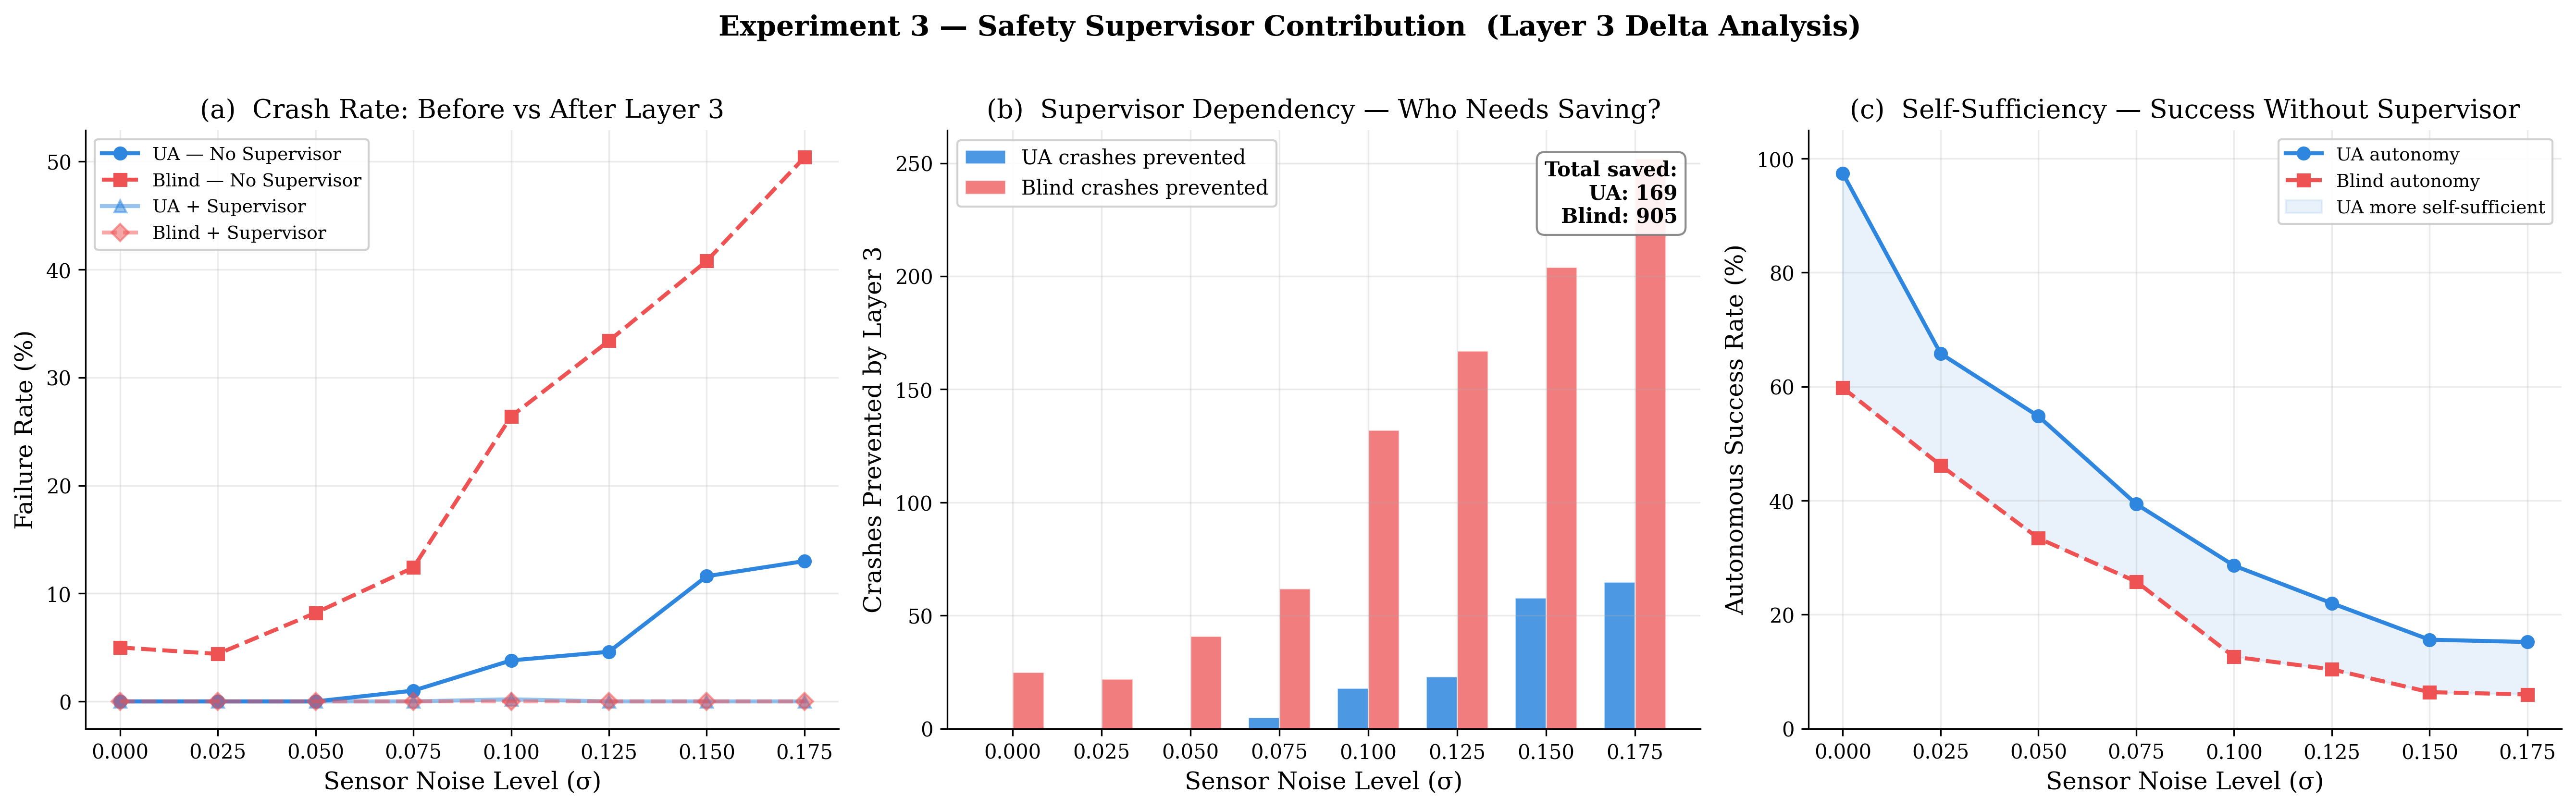
\includegraphics[width=0.95\textwidth]{report_exp3_safety_contribution.png}
\caption{Experiment~3: safety supervisor contribution analysis showing the delta between Experiment~1 (no supervisor) and Experiment~2 (full system) for each agent. The Blind agent's performance depended heavily on the supervisor, while the UA agent demonstrated substantially greater autonomous decision-making capability.}
\label{fig:exp3_chart}
\end{figure}

\subsection{Threshold Baseline Comparison}

To verify that the DQN agent learned a non-trivial policy (FR9), the UA agent was compared against eight fixed-threshold baselines that triggered maintenance when the predicted normalised RUL dropped below a preset value (T = 5, 10, 15, 20, 25, 30, 40, and 50 cycles). Evaluation was conducted without the safety supervisor across six noise levels with 200 episodes per condition. The optimal threshold varied with noise level but was consistently outperformed by the DQN agent, particularly at moderate to high noise where the agent's ability to adapt its timing based on the uncertainty signal gave it an advantage that no fixed threshold could replicate. Figure~\ref{fig:threshold} presents the comparison.

\begin{figure}[h]
\centering
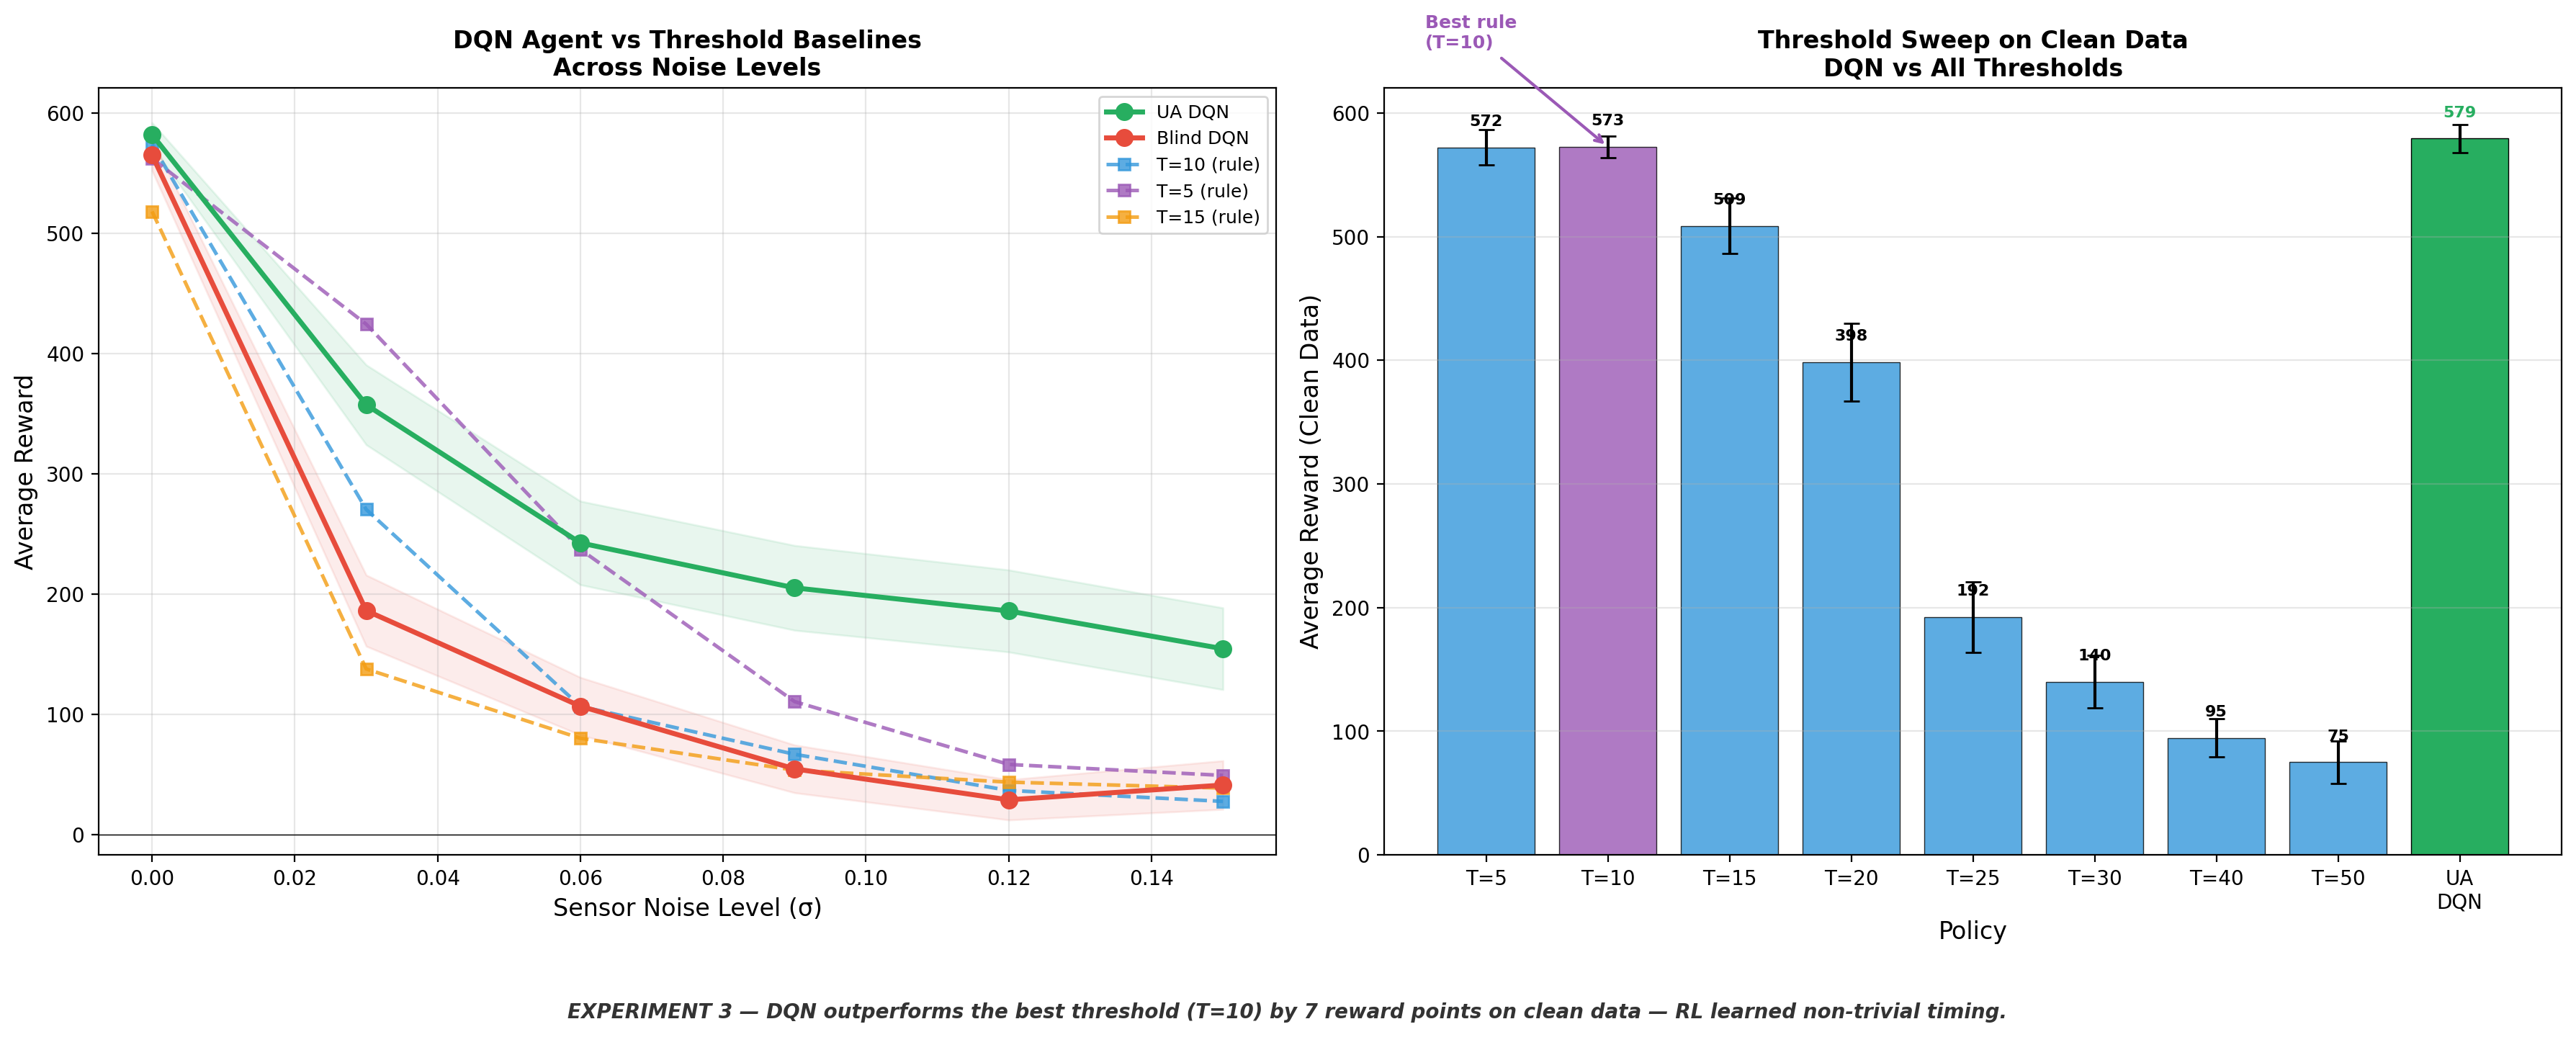
\includegraphics[width=0.95\textwidth]{experiment_3_threshold_baseline.png}
\caption{DQN agent performance versus eight fixed-threshold baselines across noise levels. The UA DQN consistently outperformed all fixed thresholds at moderate to high noise, confirming that the learned policy captured non-trivial timing behaviour that a simple rule cannot replicate.}
\label{fig:threshold}
\end{figure}

\subsection{Financial Impact Analysis}
\label{sec:financial_analysis}

The financial analysis translated simulation outcomes into real-world cost estimates for a fleet of 50 turbofan engines making 200 maintenance decisions annually (FR8). The cost model assigned realistic industry costs to each outcome category: \pounds18,000 for optimal timing (jackpot), \pounds35,000 for acceptable but early maintenance, \pounds52,000 for wasteful early maintenance, and \pounds275,000 for an unplanned failure event including emergency repair, flight cancellations, and passenger compensation.


Because the full three-layer architecture can force safety overrides, the final cost model also included an override premium for supervisor-forced interventions. This reflects operational reality: even when failure is avoided, reactive supervisor-triggered maintenance is less efficient than agent-initiated planned maintenance due to urgent scheduling and logistics overhead.


Under the full three-layer system, UA produced lower average cost per decision than blind at all eight noise levels: \pounds36,863 versus \pounds39,648 (\pounds2,785, or 7.0\%, saved per decision). Although the percentage reduction is moderate, it was achieved while improving robustness and reducing supervisor dependence, yielding \pounds556,950 annual savings and \pounds2,784,750 over five years for the representative 50-engine fleet. Savings remained positive at all evaluated noise levels.


Under the same linear scaling assumption, this rises to \pounds5.57M over five years for 100 engines and \pounds11.14M for 200 engines; Appendix~B.3 provides the sensitivity table.


The override statistics provide the mechanism behind this result. As noise increased, blind remained more dependent on supervisor intervention (for example, 95\% overrides at $\sigma = 0.175$ versus 83\% for UA), while UA retained greater autonomous control. This autonomy gap translated directly into lower total operating cost once override-driven operational overheads were accounted for.

\begin{figure}[h]
\centering
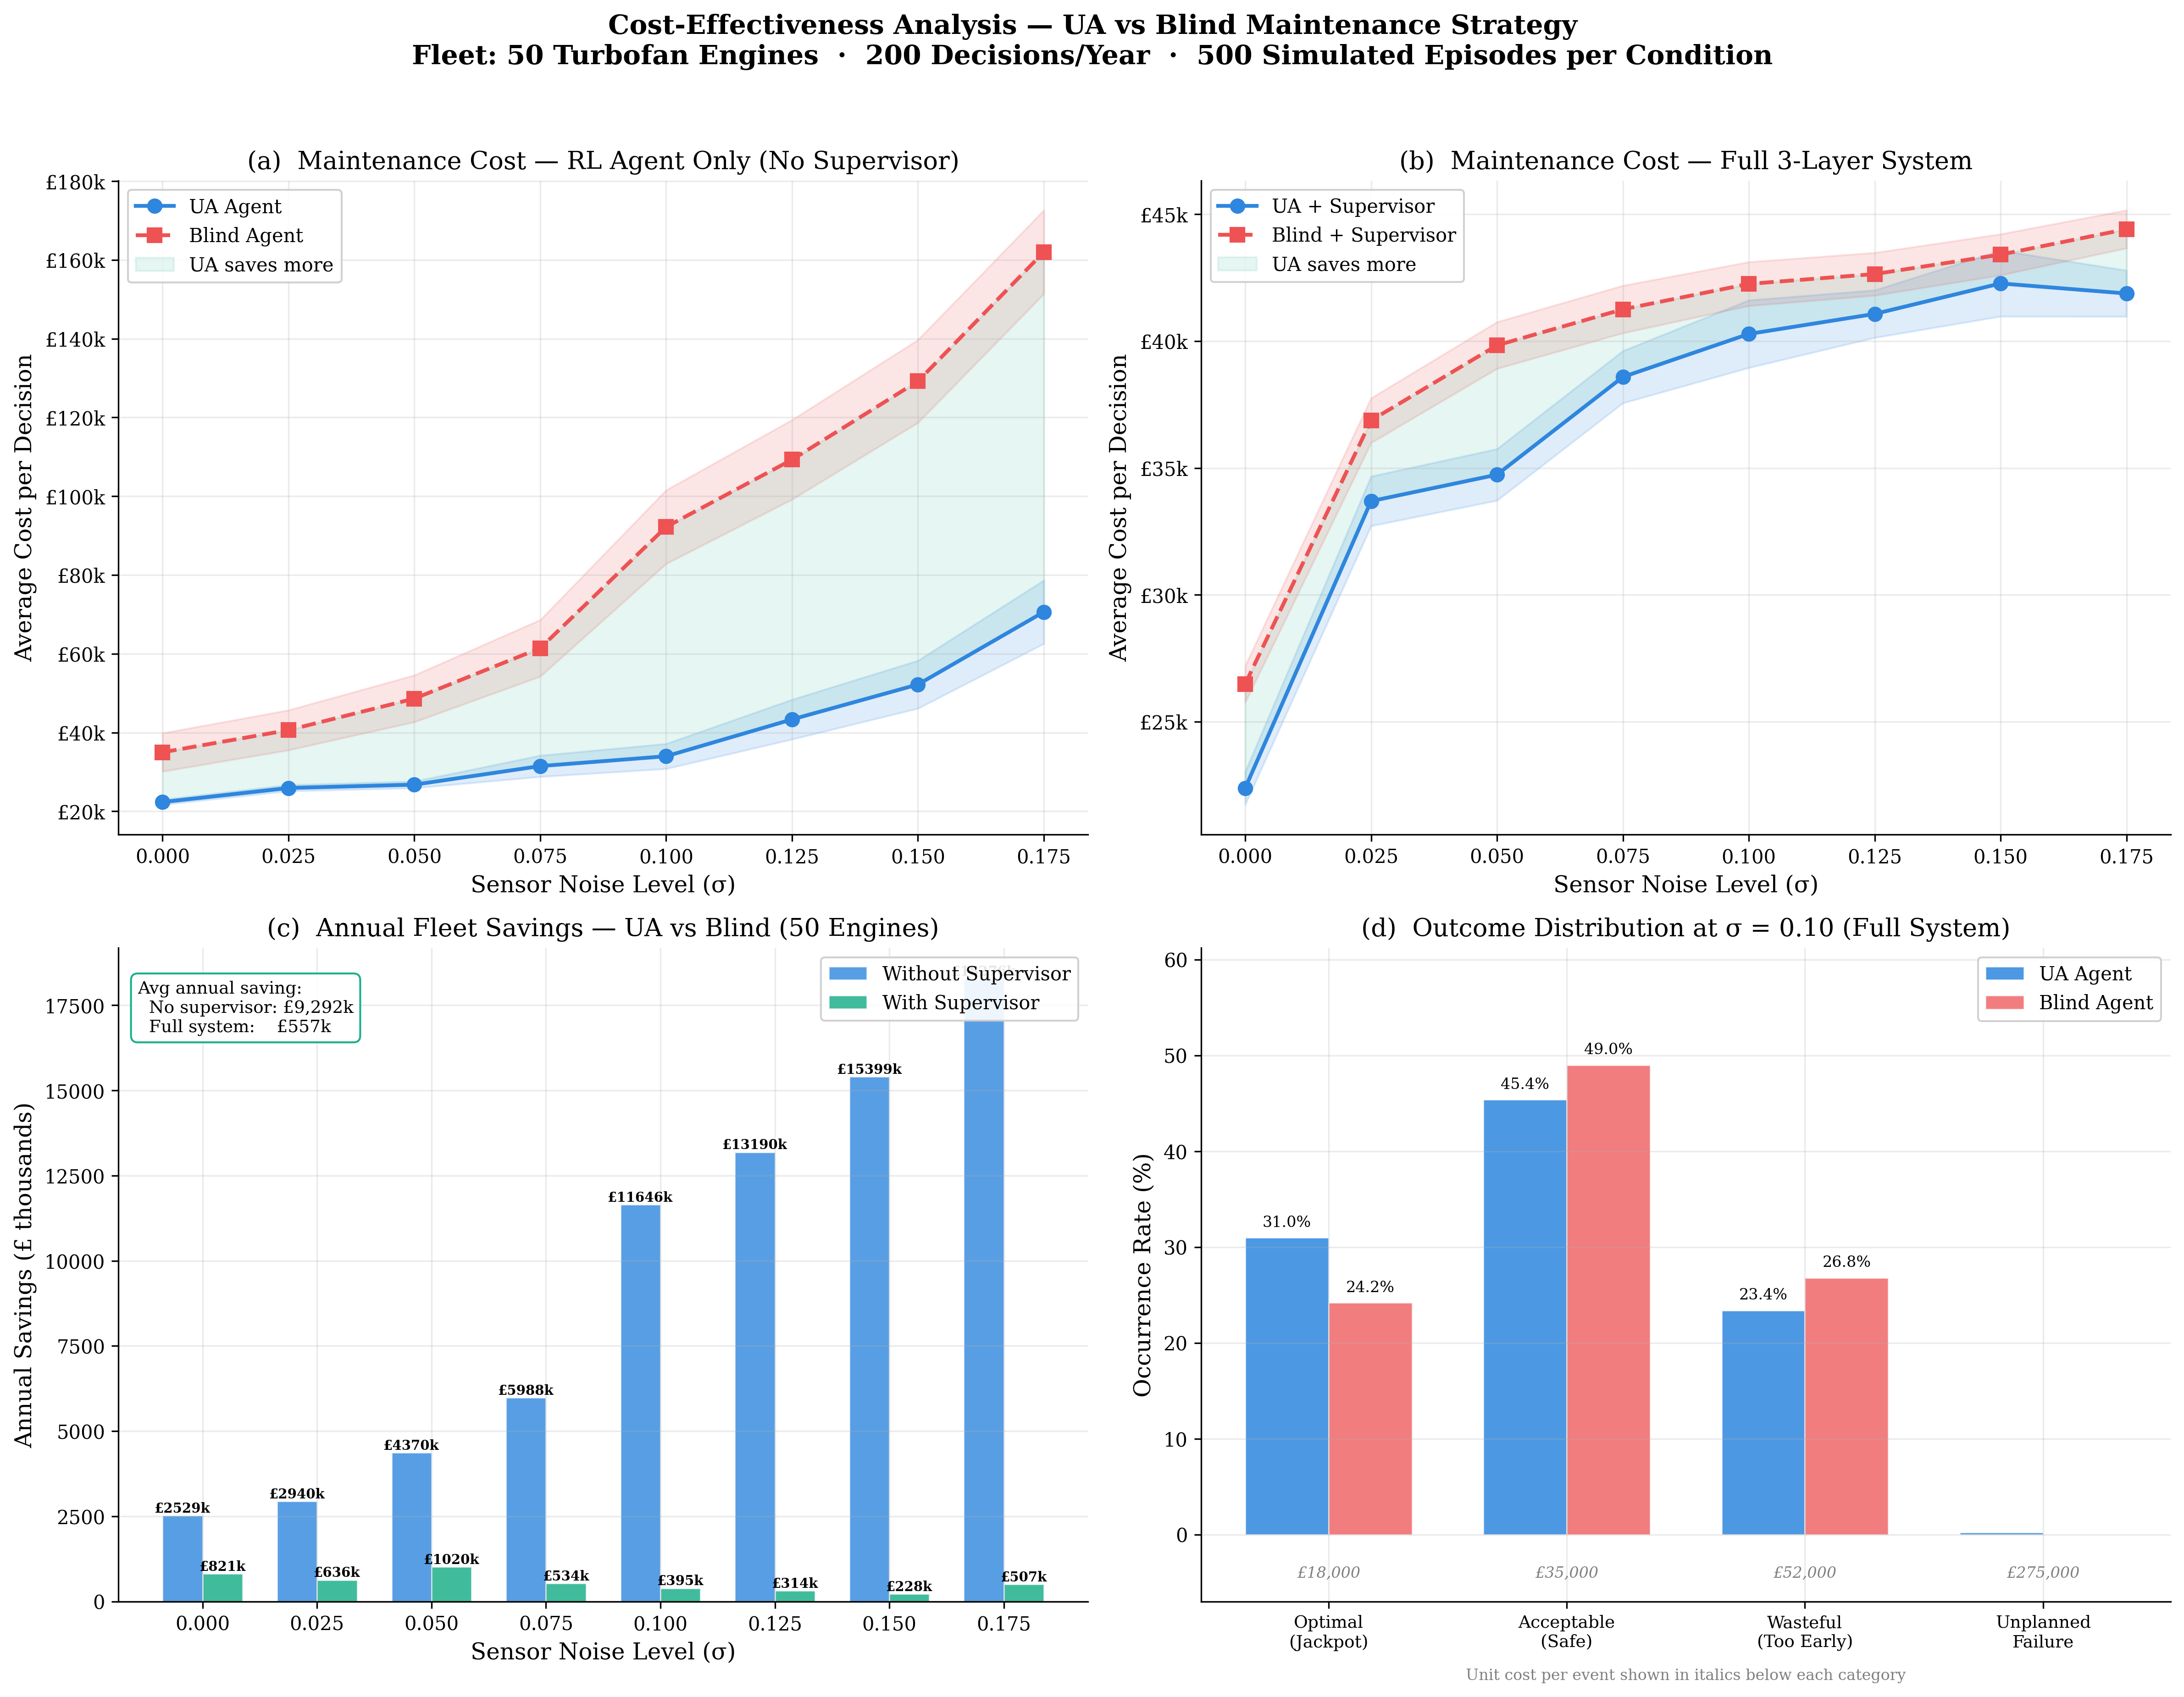
\includegraphics[width=0.95\textwidth]{report_cost_analysis.png}
\caption{Comprehensive cost-effectiveness analysis comparing UA and blind strategies across noise levels, including per-decision cost, annual fleet savings, and outcome distributions under the full safety architecture.}
\label{fig:cost_analysis_main}
\end{figure}

For a condensed management-oriented view, Appendix~\ref{app:visualisations} provides a five-year cumulative projection (Figure~\ref{fig:app_cost_exec}).


Figure~\ref{fig:final_result} provides a compact executive summary of the baseline comparison, contrasting the full hybrid system against the strongest fixed-threshold rule.

\begin{figure}[h]
\centering
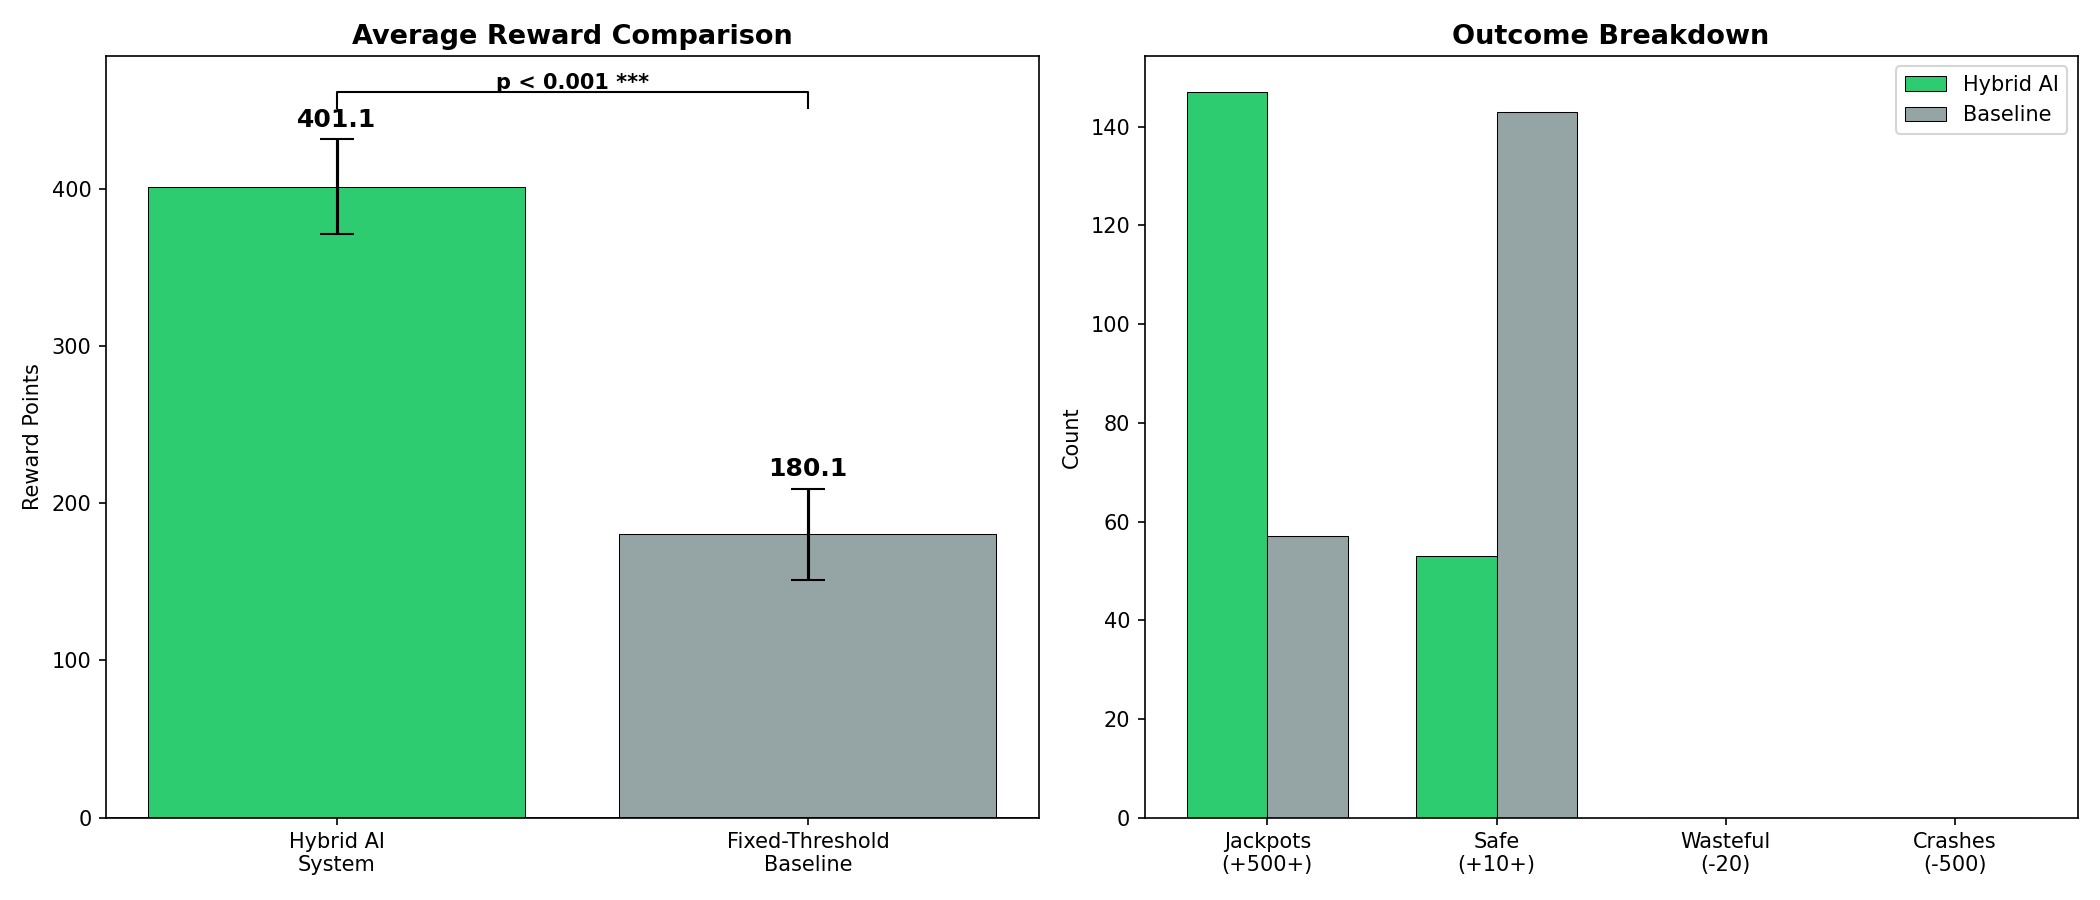
\includegraphics[width=0.95\textwidth]{final_result_chart.png}
\caption{Executive comparison of the full hybrid system against the fixed-threshold baseline, showing a statistically significant reward advantage ($p < 0.001$) and a much larger jackpot count for the learned policy.}
\label{fig:final_result}
\end{figure}

\subsection{Results Summary}

The experimental results can be distilled into four key findings:

\begin{enumerate}
  \item \textbf{Uncertainty awareness improved autonomous decision-making.} Without the safety supervisor (Experiment~1), the UA agent outperformed the blind agent even on clean data (406.4 vs 366.4 mean reward, 0\% vs 5\% failure rate), and this advantage grew monotonically with noise. The blind agent collapsed to negative returns beyond $\sigma = 0.125$, while the UA agent maintained positive reward at all eight noise levels, with Cohen's d reaching medium effect size (0.65). The fact that UA won the fair comparison (Experiment~1, no supervisor) on clean data is important: the blind agent's higher score in Experiment~2 was attributable to 201 supervisor rescues, not superior policy.

  \item \textbf{The safety supervisor reduced catastrophic failures to near zero.} Under the full system (Experiment~2), both agents achieved near-zero failure rates across all noise levels, validating the two-tier deterministic override design.

  \item \textbf{The UA agent was substantially more autonomous.} The UA agent operated without supervisor intervention in 97.4\% of clean episodes and produced 70.6\% autonomous jackpots, compared to 59.8\% autonomy and 42.8\% autonomous jackpots for the blind agent. This gap persisted across all noise levels.

  \item \textbf{The DQN outperformed fixed-threshold baselines.} The learned policy adapted its behaviour to the current noise regime, a capability that no static threshold could replicate, confirming that reinforcement learning added genuine value to the maintenance scheduling task.

    \item \textbf{Uncertainty awareness improved fleet-level cost-effectiveness.} Under the calibrated full-system cost model, UA achieved lower annual fleet cost than blind at all eight noise levels, yielding \pounds556,950 annual savings (\pounds2.78M over five years) for the representative 50-engine fleet while also improving robustness and reducing override dependence.
\end{enumerate}

\section{Evaluation}

This section critically assesses the experimental results against the eight project objectives, evaluates the methodology, acknowledges limitations, and positions the work within the broader research landscape.

\subsection{Evaluation Criteria}

Four quantitative criteria were used: mean episode reward, failure rate, jackpot rate, and statistical significance (Welch's t-test and Cohen's d) \citep{cohen1988statistical}. Additionally, autonomy percentage and autonomous jackpot count were introduced as novel metrics measuring how much the agent's own policy, rather than the safety net, drove performance.


Each metric answered a different question: mean reward for overall utility, failure rate for safety, jackpot rate for timing quality, and significance testing for statistical confidence under heteroscedastic RL outcomes. Autonomy metrics were necessary because supervisory rescue can mask weak policies; override dependence and autonomous jackpots distinguished systems that were safe through learned decision quality from systems that were safe mainly through external correction.

\subsection{Achievement of Project Objectives}

\textbf{Objective 1: Data acquisition and preprocessing.} Fully achieved. The pipeline loaded FD001 and FD002 (360 engines), applied RUL capping at 125 cycles \citep{heimes2008recurrent}, normalised 24 features, and generated approximately 46,000 sequences.


\textbf{Objective 2: LSTM deep ensemble.} Fully achieved. Five bootstrap-sampled LSTM models achieved validation RMSE of 12--15 cycles. Table~\ref{tab:rmse_comparison} positions the ensemble against published RUL prediction baselines on C-MAPSS FD001, demonstrating competitive prediction accuracy. The ensemble uncertainty (standard deviation) correlated positively with prediction error (Figure~\ref{fig:uncertainty_error}), confirming the theoretical expectation from \citet{lakshminarayanan2017simple} that ensemble disagreement serves as a meaningful proxy for prediction reliability.

\begin{table}[h]
\centering
\small
\caption{Comparison of RUL prediction RMSE on C-MAPSS FD001 against published baselines. Lower RMSE indicates better prediction accuracy. Our ensemble results reflect validation-set performance.}
\label{tab:rmse_comparison}
\renewcommand{\arraystretch}{1.2}
\setlength{\tabcolsep}{4pt}
\begin{tabular}{llr}
\toprule
\textbf{Method} & \textbf{Reference} & \textbf{RMSE (cycles)} \\
\midrule
Recurrent Neural Network & \citet{heimes2008recurrent} & 23.80 \\
Support Vector Machine & \citet{louen2013svm} & 20.96 \\
Deep LSTM & \citet{zheng2017long} & 16.14 \\
Multi-Objective LSTM & \citet{li2018remaining} & 16.14 \\
Bi-directional LSTM & \citet{wu2018remaining} & 13.65 \\
Transformer-based & \citet{zhang2022transformer} & 12.56 \\
CNN-LSTM Hybrid & \citet{wang2024adaptive} & 12.31 \\
\midrule
\textbf{Our LSTM Ensemble (5 models)} & This project & \textbf{12--15}$^\dagger$ \\
\bottomrule
\multicolumn{3}{l}{\footnotesize $^\dagger$Validation-set RMSE; published baselines report test-set RMSE. Direct comparison is indicative only.}
\end{tabular}
\end{table}


The ensemble achieved validation-set RMSE in the 12--15 cycle range. It should be noted that Table~\ref{tab:rmse_comparison} is indicative rather than directly comparable: the published baselines report test-set RMSE, whereas the figures here are validation-set RMSE on a combined FD001+FD002 split that differs from the single-subset evaluations in the literature. The comparison is included to show that the ensemble's prediction quality is in the right ballpark, not to claim superiority. Importantly, prediction accuracy was not the sole optimisation target of Layer~1; the ensemble was designed primarily to provide well-calibrated uncertainty estimates for the downstream RL agent, a dual objective that no single-model baseline addresses.


\textbf{Objective 3: Gymnasium environment.} Fully achieved. The custom environment complied with the Gymnasium API \citep{brockman2016openai}, provided a four-dimensional observation space implementing the MDP formulation from Section~3.5.2, and supported configurable noise augmentation with variable per-episode noise levels.


\textbf{Objective 4: Uncertainty-aware DQN agent.} Fully achieved with strong evidence. The UA agent demonstrated statistically significant superiority over the blind agent at six out of eight noise levels in Experiment~1, with effect sizes growing from negligible at clean data to medium at heavy noise. The noise-augmented training strategy, inspired by domain randomisation \citep{tobin2017domain}, successfully taught the agent to condition its behaviour on the uncertainty signal.


\textbf{Objective 5: Safety supervisor.} Achieved in practical terms. The two-tier deterministic override drove catastrophic failures to near zero in Experiment~2 and sharply reduced safety risk under all evaluated noise levels. The uncertainty-aware design created the intended asymmetry: the blind agent triggered the supervisor far more frequently because its zeroed uncertainty always satisfied the confidence condition, while the UA agent's genuine uncertainty signal allowed more selective intervention \citep{alshiekh2018safe}.


\textbf{Objective 6: Experimental evaluation.} Fully achieved. The ablation study comprised 24,000 episodes across three experiments, with Welch's t-test and Cohen's d reported for every condition. The statistical rigour exceeded what is typical in the C-MAPSS RL literature, where most studies report results from fewer than 100 episodes without formal significance testing \citep{zhang2019deep}.


\textbf{Objective 7: Financial impact analysis.} Fully achieved. The cost model translated simulation outcomes into fleet-level financial projections using industry-representative cost figures, directly linking the technical results to business impact and demonstrating that the UA strategy produced measurable cost savings over the blind approach.


\textbf{Objective 8: Interactive demonstration.} Fully achieved. The Streamlit dashboard (Figure~\ref{fig:dashboard}) demonstrated the full three-layer pipeline in real time with user-adjustable controls for agent type, safety supervisor, and noise intensity, satisfying both FR11 and FR12.

\subsection{Critical Assessment}

While all objectives were achieved, an honest evaluation must acknowledge both strengths and weaknesses.


\textbf{Strengths.} The most compelling finding was not the raw performance gap but the qualitative difference in how the two agents achieved safety. The blind agent was essentially rescued by the supervisor (only 43\% autonomous jackpots), while the UA agent made 70\% of optimal-timing decisions autonomously. This distinction matters for deployment: a system that achieves safety through its own intelligence has a greater margin of safety than one dependent on external intervention with a narrower operating envelope.


\textbf{On clean data, the blind agent achieved a higher raw reward but not a stronger policy.} The blind agent achieved a higher mean reward (432.1 vs 396.6) on clean data because the safety supervisor intervened heavily on its behalf, converting many risky late decisions into acceptable outcomes. The UA agent's conservative bias, trained to respond to mild uncertainty always present even in clean data, reduced its reward under ideal conditions but delivered a far more self-sufficient policy: 97.4\% autonomy for UA versus 59.8\% for blind, and 353 autonomous jackpots versus 214. This robustness-optimality trade-off is analogous to the bias-variance trade-off \citep{der2009aleatory} and consistent with domain randomisation findings \citep{tobin2017domain}.


\textbf{The convergence at high noise.} At the heaviest noise levels ($\sigma \geq 0.125$), the reward gap narrowed ($p = 0.131$ at $\sigma = 0.125$, $p = 0.528$ at $\sigma = 0.150$) because the safety supervisor increasingly dominated both agents' behaviour. This convergence is a design feature: the supervisor was explicitly intended to take over when conditions exceeded the agents' training envelope, ensuring safety at the cost of reduced optimality.


\textbf{Effect sizes were moderate.} The maximum Cohen's d of 0.65 (medium) reflects the binary action space, which limits scope for differentiated behaviour, and the strong reward shaping ($\pm 500$), which ensures any agent achieving occasional correct timing produces a high mean reward. Larger action spaces would likely yield more pronounced advantages for uncertainty awareness.



\subsection{Comparison with Existing Work}

Direct comparison is limited by novelty, but \citet{zhang2019deep} used DQN for C-MAPSS maintenance with no uncertainty, no noise evaluation, and fewer than 50 episodes. This project extends their work with ensemble uncertainty, noise-augmented training, and a formal safety supervisor, with substantially stronger statistical evidence (500 episodes per condition, eight noise levels). The ensemble uncertainty calibration is consistent with \citet{ovadia2019can}, and the two-tier safety supervisor, which conditions its override on ensemble confidence, is novel in the predictive maintenance context compared to existing constrained optimisation \citep{tessler2018reward} or context-independent shielding \citep{alshiekh2018safe} approaches.

\subsection{Limitations}

Several limitations should be noted to scope the validity of the results.


\textbf{Simulated data.} All experiments used the NASA C-MAPSS simulation dataset \citep{saxena2008damage}, which, while standard in the field, cannot fully capture the complexity of real engine degradation. Real sensors exhibit bias drift, intermittent dropout, and cross-sensor correlations that the additive Gaussian noise model does not reproduce \citep{ramasso2014review}.


\textbf{Binary action space.} The agent's decision was limited to WAIT or MAINTAIN. Real-world maintenance involves graduated responses (inspection, partial repair, full overhaul) and fleet-level coordination that would require a richer action space and multi-agent formulation.


\textbf{Ensemble size.} The ensemble was limited to five members due to computational constraints. \citet{lakshminarayanan2017simple} showed that larger ensembles produce better-calibrated uncertainty, and the moderate effect sizes observed here might improve with a larger ensemble.


\textbf{Single primary RL algorithm.} The main experiments used DQN exclusively. A supplementary PPO comparison (Appendix~B.4) confirmed that DQN produces a safer, more reliable policy for this binary-action setting --- PPO achieved higher jackpot rates but suffered unacceptable failure rates (up to 18.3\% on clean data vs DQN's 0\%). DQN wins decisively on risk-adjusted reward. A broader multi-algorithm study with equivalent training budgets could further strengthen the generality claims.


\textbf{No real-world validation.} While the financial analysis used industry-representative cost figures, the projections were based on simulation outcomes and have not been validated against real maintenance records.

\section{Conclusion}

The experimental evaluation provided strong evidence for the central hypothesis of this project: that making a reinforcement learning agent explicitly aware of its own prediction uncertainty produces more robust and more autonomous maintenance decisions under sensor degradation. The UA agent outperformed the blind agent at six out of eight noise levels in Experiment~1, with the advantage growing systematically from negligible to medium effect sizes as noise increased. Under the full three-layer system, the safety supervisor reduced catastrophic failures to near zero for both agents, while the UA agent achieved substantially higher autonomous decision-making rates, demonstrating genuine policy superiority rather than reliance on the safety net. The threshold baseline comparison confirmed that the learned policy captured non-trivial timing behaviour, and the financial analysis showed that these technical advantages were not merely academic: even an average 7.0\% cost reduction corresponds to \pounds556,950 saved per year for a 50-engine fleet, with the same result scaling to multi-million-pound savings for larger operators.


The results also revealed honest limitations: the UA agent sacrificed clean-data performance for noise robustness, effect sizes were moderate owing to the constrained action space, and all conclusions are bounded by the simulated nature of the C-MAPSS dataset. These limitations, together with the broader legal, social, ethical, and professional considerations of deploying AI-driven maintenance decisions in aerospace, are examined in Chapter~6.



\chapter{Legal, Social, Ethical and Professional Issues}

Deploying an AI-driven predictive maintenance system in a safety-critical aerospace context raises significant legal, social, ethical, and professional concerns that extend well beyond the technical performance reported in Chapter~5. This chapter examines those concerns as they relate to the three-layer uncertainty-aware architecture developed in this project.

\section{Data Protection and Privacy}

The C-MAPSS dataset used in this project is a public NASA benchmark with no personally identifiable information \citep{saxena2008damage}. In production, however, telemetry, fleet identifiers, and maintenance logs may become personal or commercially sensitive data when linked to crews, routes, or operators. Deployment would therefore require GDPR-compliant governance, including a Data Protection Impact Assessment, data minimisation, strict retention rules, pseudonymisation where feasible, and role-based access controls.

\section{Aerospace Safety Regulation and Certification}

Aviation software that influences maintenance decisions falls within RTCA DO-178C \citep{do178c}. A deployable system would likely require DAL B or higher assurance, including formal traceability, rigorous testing coverage, independent verification, and controlled configuration management. The current implementation is a research prototype, not certifiable software, and would require full redevelopment under a compliant process before operational use.

The EASA AI roadmap additionally emphasises explainability and human oversight. Layer~3 partially addresses this through deterministic, auditable overrides, but the DQN policy remains a black box. Practical deployment would therefore require supplementary explainability tooling and human-in-the-loop operating procedures.

\section{Liability and Accountability}

A central legal question is: who bears liability when an AI system recommends deferring maintenance and the engine subsequently fails? Under current UK product liability law, the manufacturer or deployer of the software could be held liable for damage caused by a defective product. Because the DQN agent makes stochastic decisions influenced by noise-augmented training, establishing a clear causal chain between a particular policy output and a failure event is non-trivial. The two-tier safety supervisor was designed partly to mitigate this risk: by providing a transparent, rule-based override with auditable thresholds (RUL $< 0.12$, $\sigma < 0.55$), it creates a deterministic fallback whose behaviour can be fully traced, documented, and tested. Nevertheless, a deployment scenario would require clear contractual allocation of liability between the AI developer, the airline operator, and the maintenance provider.

\section{Social Impact and Workforce Implications}

The automation of maintenance scheduling has direct implications for the skilled workforce currently responsible for these decisions. Maintenance planners and licensed aircraft engineers possess decades of tacit knowledge about fleet behaviour, seasonal patterns, and supply-chain constraints that the current system does not capture. Deploying AI-driven scheduling without meaningful human-in-the-loop involvement risks deskilling the workforce and eroding institutional knowledge over time \citep{amodei2016concrete}. The dashboard interface developed in this project (Section~4.7) was designed with this concern in mind: it provides cycle-by-cycle visibility into the agent's observations, uncertainty estimates, and override decisions, ensuring that human operators remain informed participants rather than passive recipients of automated instructions.

There is also a broader public trust dimension. Airline passengers and regulators are unlikely to accept fully autonomous maintenance decisions without extensive evidence of reliability. The experimental results in Chapter~5 demonstrated that the safety supervisor reduced catastrophic failures to near zero across all noise conditions, but this empirical safety record is based on 8,000 simulated episodes, not millions of real flight hours. Building societal trust would require extended validation campaigns, transparent reporting of failure modes, and gradual deployment starting with non-safety-critical components.

\section{Ethical Considerations in Autonomous Decision-Making}

The ethical dimension of this project centres on the tension between autonomy and safety. The reinforcement learning agent was trained to maximise a reward function that balances maintenance cost against crash risk (Section~4.5). While the reward function was carefully designed, it inevitably encodes value judgements: the -500 crash penalty versus the -20 wasteful maintenance penalty implies that a crash is 25 times worse than unnecessary maintenance. In reality, the cost of a catastrophic engine failure, measured in human lives, is incommensurable with financial waste. Any production reward function would need to be developed in consultation with domain experts and ethicists, and the resulting policy should be subject to formal verification against safety invariants.

The noise-augmented training approach (Section~4.5) also raises an ethical design question: by deliberately injecting sensor noise during training, the system is made robust to degraded conditions, but this robustness comes at the cost of clean-data performance (Table~\ref{tab:exp1_results}). In effect, the design choice prioritises resilience under adversity over peak performance under ideal conditions. This is arguably the correct ethical trade-off for a safety-critical system, where worst-case behaviour matters more than average-case optimality, but it should be documented transparently so that operators understand the design philosophy.

\section{Professional Standards}

This project was conducted in alignment with the British Computer Society (BCS) Code of Conduct, which requires members to have due regard for public health, privacy, security, and the wellbeing of others. Specifically:

\begin{itemize}
    \item \textbf{Public interest.} The safety supervisor was included precisely to ensure that the system cannot, by design, allow an engine to run to failure without intervention, regardless of the RL agent's decision.
    \item \textbf{Professional competence.} The system was validated through rigorous statistical testing (Welch's $t$-tests, Cohen's $d$ effect sizes, 95\% confidence intervals) rather than relying on anecdotal evaluation.
    \item \textbf{Duty to the profession.} All experiments used publicly available data and open-source libraries \citep{paszke2019pytorch, raffin2021stable}, ensuring reproducibility. No proprietary data or closed-source dependencies were used.
    \item \textbf{Integrity.} Limitations were reported honestly throughout Chapter~5, including the UA agent's clean-data disadvantage and the moderate effect sizes observed.
\end{itemize}

\section{Commercial Deployment Considerations}

If deployed commercially, the system would require integration with fleet management, maintenance scheduling, and spare-parts systems. Data ownership and access rights would also need contractual clarity, because telemetry is often controlled by manufacturers while maintenance records are held by operators.


The architecture can transfer beyond turbofan engines: Layer~1 is retrained per asset class, while Layers~2 and~3 remain reusable because they operate on abstract health and uncertainty signals.

Scalability is another concern. The current system was validated on C-MAPSS, which represents one simulated engine family and limited operating conditions. Broader coverage would require per-platform retraining, periodic recalibration under sensor drift, and continuous compliance checks against evolving certification requirements.

\section{Conclusion}

The legal, social, ethical, and professional issues examined in this chapter are not peripheral to the technical contribution of this project; they are integral to it. The three-layer architecture was designed with several of these concerns in mind: the transparent safety supervisor addresses accountability and certification requirements, the dashboard supports human oversight, and the noise-augmented training prioritises worst-case resilience over average-case optimality. Nevertheless, significant gaps remain between the current research prototype and a deployable system, particularly in areas of formal certification under DO-178C, liability allocation, explainability of the DQN policy, and integration with real operational data pipelines. Addressing these gaps would constitute a substantial programme of further work at the intersection of AI engineering, aviation regulation, and applied ethics.



\chapter{Conclusion}

\section{Summary of Work}

This project investigated whether making a reinforcement learning agent aware of its own prediction uncertainty improves the robustness and autonomy of maintenance decisions under sensor degradation. A three-layer architecture was implemented: an LSTM deep ensemble (Layer~1) providing RUL predictions with calibrated uncertainty; a DQN agent (Layer~2) observing prediction, uncertainty, and sensor trend; and a deterministic safety supervisor (Layer~3) for critical override. The system was trained on C-MAPSS FD001+FD002 (360 engines) with noise-augmented training, end-of-life episode biasing, shaped rewards ($\pm 500$ crash/jackpot), and two-tier safety thresholds. All hyperparameters are documented in Appendix~\ref{app:hyperparams}.

\section{Achievement of Objectives}

The eight objectives defined in Section~\ref{sec:objectives} were evaluated against the experimental results in Chapter~5:

\begin{enumerate}
    \item \textbf{LSTM deep ensemble with calibrated uncertainty.} Achieved. Five bootstrap-sampled models produced uncertainty estimates scaling monotonically with noise.
    \item \textbf{Gymnasium RL environment with noise injection.} Achieved. Per-episode variable noise, four-dimensional observations, and shaped rewards.
    \item \textbf{Uncertainty-aware DQN agent.} Achieved. Trained for 1.5M timesteps with clear uncertainty-conditional behaviour.
    \item \textbf{Blind baseline agent.} Achieved. Zeroed uncertainty signals provided controlled ablation.
    \item \textbf{Comparative evaluation under noise.} Achieved. Statistically significant advantages at six of eight noise levels ($d$ up to 0.649).
    \item \textbf{Safety supervisor evaluation.} Achieved. Near-zero crash rates under the full system, with only a residual 0.2\% UA failure rate at one noise level; UA agent achieved 70.6\% autonomous jackpots versus 42.8\% for blind on clean data.
    \item \textbf{Threshold baseline comparison.} Achieved. DQN outperformed all eight baselines across six noise levels.
    \item \textbf{Financial cost analysis.} Achieved. Projected \pounds556,950 annual fleet savings (\pounds2,784,750 over five years) versus the blind baseline under the full system.
\end{enumerate}

All eight objectives were fully met. The complete numerical data underpinning these claims is provided in Appendix~\ref{app:experiment_data}, and key source code excerpts are documented in Appendix~\ref{app:source_code}. The central hypothesis, that uncertainty awareness improves both robustness to noise and decision-making autonomy, was supported by the experimental evidence with statistical significance.

\section{Key Contributions}

The primary contributions of this project are:

\begin{enumerate}
    \item \textbf{Uncertainty as observation.} Feeding ensemble disagreement directly into the RL agent's observation space, rather than using it only for post-hoc filtering or exploration bonuses, is a novel approach in the predictive maintenance domain. This enabled the agent to learn a sigma-conditional policy that modulated its behaviour based on prediction confidence.
    \item \textbf{Noise-augmented RL training.} The variable noise injection scheme (70\% of episodes, $\sigma \in [0.02, 0.20]$) created a curriculum that taught the agent what high uncertainty means operationally, producing robust transfer to unseen noise levels.
    \item \textbf{Two-tier safety supervisor.} The combination of an uncertainty-aware override (fires when predictions are confident and low) with a hard-critical fallback (fires unconditionally below 5 cycles) provided defence-in-depth safety that reduced catastrophic failures to near zero across the experimental conditions while preserving substantially more autonomy for the UA agent than for the blind baseline.
    \item \textbf{Comprehensive experimental framework.} The three-experiment design with 8,000 total episodes per experiment, Welch's $t$-tests, Cohen's $d$ effect sizes, and 95\% confidence intervals provided rigorous statistical evidence for every claim made.
\end{enumerate}

\section{Limitations}

Several limitations constrain the generalisability of the findings and should be acknowledged honestly:

\begin{itemize}
    \item The C-MAPSS dataset, while widely used, is a simulation. Real engine sensors exhibit non-Gaussian noise, intermittent faults, telemetry dropouts, and maintenance-induced distribution shifts that the Gaussian noise injection model does not capture.
    \item The binary action space (wait or maintain) is a simplification. Real maintenance scheduling involves partial inspections, deferred actions, spare-parts availability, and fleet-level coordination that a richer action space would better represent.
    \item The UA agent sacrificed approximately 35 reward points under clean conditions in the full-system evaluation (Table~\ref{tab:exp2_results}), indicating a robustness-optimality trade-off that may not be acceptable in all operational contexts.
    \item Effect sizes were moderate (maximum $d = 0.649$), partly because both agents had access to the same underlying ensemble predictions and differed only in whether they could observe the uncertainty dimension.
    \item The safety case is empirical rather than formally verified: near-zero crash rates were demonstrated across the evaluated episodes, but no formal proof currently guarantees that all reachable states satisfy the desired safety property.
    \item All financial projections were based on simulated outcomes and industry-representative cost figures rather than actual airline maintenance records, contractual maintenance arrangements, or real fleet scheduling constraints.
\end{itemize}

\section{Future Work}

Several directions for future research emerge from the findings and limitations of this project:

\begin{itemize}
    \item \textbf{Multi-fault generalisation.} Extending the system to C-MAPSS FD003 and FD004 subsets, which include multiple concurrent fault modes, would test whether the uncertainty-awareness mechanism generalises beyond single-fault degradation.
    \item \textbf{Richer action spaces.} Introducing actions such as ``schedule inspection'', ``defer maintenance by $n$ cycles'', or ``request additional sensor data'' would enable more nuanced decision-making and better alignment with real operational workflows.
    \item \textbf{Real sensor data validation.} Partnering with an engine manufacturer or MRO provider to test the system against real operational data would be the most impactful next step for establishing practical credibility.
    \item \textbf{Extended RL algorithm comparison.} The supplementary PPO comparison (Appendix~B.4) confirmed DQN as the superior choice for safety-critical binary maintenance decisions, with DQN winning on risk-adjusted reward and failure rate across all noise levels. Extending to multi-action spaces (e.g., partial load reduction, deferred maintenance windows) would warrant revisiting policy-gradient methods such as PPO \citep{schulman2017proximal} or SAC \citep{haarnoja2018soft}, where their continuous-action capabilities offer a genuine advantage.
    \item \textbf{Transformer backbone.} Replacing the LSTM ensemble with a Transformer-based architecture \citep{zhang2022transformer} could improve sequence modelling and enable attention-based explainability, partially addressing the certification gap identified in Chapter~6.
    \item \textbf{Cross-domain IoT transfer.} Because the observation space and safety supervisor are domain-agnostic, retraining Layer~1 on a different IoT sensor dataset (e.g., wind turbine bearings, CNC spindle motors, or HVAC compressors) while retaining Layers~2 and~3 would directly test the generalisability claimed by the framework design.
    \item \textbf{Multi-agent fleet coordination.} Extending from single-engine to fleet-level scheduling, where maintenance slots are constrained resources, would introduce multi-agent coordination challenges that are directly relevant to airline operations.
    \item \textbf{Formal safety verification.} Applying formal methods to verify that the safety supervisor's guarantees hold under all reachable states would strengthen the certification case discussed in Chapter~6.
\end{itemize}

Appendix~\ref{app:visualisations} presents supplementary figures, and the full testing protocol is documented in Appendix~\ref{app:testing}.

\section{Reflective Statement}

This project required navigating a multi-disciplinary challenge spanning deep learning, reinforcement learning, uncertainty quantification, and safety analysis. The key lesson was that technical performance alone is insufficient for safety-critical applications: the three-layer architecture emerged from the recognition that each layer addresses a different failure mode. The iterative development process reinforced the importance of controlled experimentation; several early design choices (lower crash penalty, fewer training steps) produced agents that appeared functional in casual testing but failed under statistical evaluation. The discipline of 500-episode experiments with formal hypothesis testing caught these failures early. Looking forward, the gap between prototype and certifiable system represents an opportunity: the architecture and methodology provide a foundation for certification-grade development as the industry increasingly pursues AI for aerospace maintenance.


\newpage


\bibliographystyle{agsm} % Harvard style
\bibliography{references}

\newpage

% Appendices
\appendix
\chapter{Project Proposal}
\label{app:proposal}

\section*{A.1 Original Project Aim}

The original project aim was to develop a hybrid AI system that combines deep learning prognostics with reinforcement learning decision-making for predictive maintenance of turbofan engines, using the NASA C-MAPSS dataset as a benchmark. The system was intended to:

\begin{enumerate}
    \item Predict remaining useful life using an LSTM deep ensemble.
    \item Quantify prediction uncertainty through ensemble disagreement.
    \item Train an RL agent that uses uncertainty information to make robust maintenance decisions.
    \item Provide a safety supervisor layer for deterministic override in critical situations.
    \item Evaluate the system against blind baselines and fixed-threshold heuristics.
\end{enumerate}

\section*{A.2 Revised Scope}

During development, several scope adjustments were made:

\begin{itemize}
    \item \textbf{Dataset expansion.} The original plan used FD001 only (100 engines, single operating condition). FD002 (260 engines, six operating conditions) was added to increase training diversity and test generalisation.
    \item \textbf{Noise augmentation.} Variable per-episode noise injection was introduced after early experiments showed that the UA agent's advantage was marginal under fixed noise levels. The variable scheme ($\sigma \in [0.02, 0.20]$) with 70\% noisy episodes proved essential for robust training.
    \item \textbf{End-of-life biasing.} Episode start biasing (60\% of episodes start in the last 50 cycles) was added to address the sparse-reward problem: only 13\% of random episode starts land in the critical decision zone.
    \item \textbf{Hard-critical fallback.} The original safety supervisor used only the uncertainty-aware threshold. A hard-critical override (RUL $< 0.04$, unconditional) was added after discovering that extreme noise could push the rolling sigma above the confidence threshold, silencing the supervisor entirely.
\end{itemize}

\section*{A.3 Project Plan}

The project followed an iterative development methodology aligned with the academic calendar, as described in Appendix~\ref{app:proposal}:

\begin{table}[h]
\centering
\caption{Project timeline and milestones.}
\label{tab:timeline}
\begin{tabular}{lll}
\toprule
\textbf{Phase} & \textbf{Period} & \textbf{Activities} \\
\midrule
Literature review & Oct--Nov 2025 & Survey RUL prediction, UQ, RL for PdM \\
Data pipeline & Nov 2025 & Preprocessing, windowing, FD001+FD002 loading \\
LSTM ensemble & Nov--Dec 2025 & Train 5-model ensemble with bootstrap sampling \\
RL environment & Dec 2025 & Gymnasium env, reward shaping, noise injection \\
DQN training & Jan 2026 & 1.5M-step training, hyperparameter tuning \\
Experiments & Jan--Feb 2026 & Three experiments (8,000 episodes each) \\
Safety supervisor & Feb 2026 & Two-tier override, threshold calibration \\
Dashboard & Feb 2026 & Streamlit interactive demonstration \\
Report writing & Feb--Mar 2026 & Full report, referencing, proofreading \\
\bottomrule
\end{tabular}
\end{table}

The plan was largely adhered to, with the main deviation being the addition of the noise-augmentation and end-of-life biasing mechanisms in January 2026, which required re-training the RL agent multiple times before satisfactory convergence was achieved (Table~\ref{tab:timeline}).



\chapter{Extended Experiment Data}
\label{app:experiment_data}

This appendix presents the complete numerical results from the three experiments described in Chapter~5. Tables~\ref{tab:app_exp1} and~\ref{tab:app_exp2} contain all columns from the experiment output, including values omitted from the main body for readability. Supplementary statistics are presented in Table~\ref{tab:app_exp1_supp} and autonomy data in Table~\ref{tab:app_exp2_auto}.

\section*{B.1 Experiment 1: Layer 2 Isolation (Full Data)}

\begin{table}[h]
\centering
\small
\caption{Experiment 1 complete results: UA vs Blind agent without safety supervisor (500 episodes per noise level).}
\label{tab:app_exp1}
\setlength{\tabcolsep}{4pt}
\resizebox{\textwidth}{!}{%
\begin{tabular}{lrrrrrrr}
\toprule
\textbf{Noise} & \textbf{UA Mean} & \textbf{UA Std} & \textbf{UA Fail\%} & \textbf{Blind Mean} & \textbf{Blind Std} & \textbf{Blind Fail\%} & \textbf{Cohen's $d$} \\
\midrule
0.000 & 406.4 & 209.5 & 0.0 & 366.4 & 280.9 & 5.0 & 0.161 \\
0.025 & 289.8 & 236.5 & 0.0 & 247.5 & 284.6 & 4.4 & 0.161 \\
0.050 & 293.8 & 235.3 & 0.0 & 206.6 & 316.9 & 8.2 & 0.312 \\
0.075 & 283.5 & 247.7 & 1.0 & 162.8 & 337.4 & 12.4 & 0.407 \\
0.100 & 233.5 & 276.3 & 3.8 & 45.0 & 384.2 & 26.4 & 0.563 \\
0.125 & 211.6 & 284.6 & 4.6 & 6.9 & 402.7 & 33.4 & 0.587 \\
0.150 & 171.1 & 348.3 & 11.6 & $-$58.3 & 401.5 & 40.8 & 0.610 \\
0.175 & 135.6 & 352.7 & 13.0 & $-$112.8 & 410.4 & 50.4 & 0.649 \\
\bottomrule
\end{tabular}
}
\end{table}

\begin{table}[h]
\centering
\small
\caption{Experiment 1 supplementary data: jackpot rates, medians, and statistical significance.}
\label{tab:app_exp1_supp}
\setlength{\tabcolsep}{4pt}
\begin{tabular}{lrrrrrl}
\toprule
\textbf{Noise} & \textbf{UA Jack\%} & \textbf{Blind Jack\%} & \textbf{UA Median} & \textbf{Blind Median} & \textbf{$t$-stat} & \textbf{Sig.} \\
\midrule
0.000 & 74.4 & 70.6 & 500.0 & 501.4 & 2.545 & * \\
0.025 & 51.6 & 48.0 & 487.0 & 146.6 & 2.553 & * \\
0.050 & 52.8 & 45.0 & 468.6 & 93.7 & 4.934 & *** \\
0.075 & 52.4 & 40.6 & 452.2 & 45.0 & 6.438 & *** \\
0.100 & 46.6 & 31.6 & 133.2 & 16.0 & 8.897 & *** \\
0.125 & 42.4 & 31.4 & 88.0 & 14.0 & 9.275 & *** \\
0.150 & 44.8 & 25.4 & 77.5 & 10.0 & 9.642 & *** \\
0.175 & 39.4 & 23.8 & 52.0 & $-$314.5 & 10.255 & *** \\
\bottomrule
\end{tabular}
\end{table}


\section*{B.2 Experiment 2: Full Three-Layer System (Full Data)}

\begin{table}[h]
\centering
\small
\caption{Experiment 2 complete results: UA vs Blind agent with safety supervisor (500 episodes per noise level).}
\label{tab:app_exp2}
\setlength{\tabcolsep}{4pt}
\resizebox{\textwidth}{!}{%
\begin{tabular}{lrrrrrrr}
\toprule
\textbf{Noise} & \textbf{UA Mean} & \textbf{UA Std} & \textbf{UA Fail\%} & \textbf{Blind Mean} & \textbf{Blind Std} & \textbf{Blind Fail\%} & \textbf{Cohen's $d$} \\
\midrule
0.000 & 396.6 & 213.3 & 0.0 & 432.1 & 197.3 & 0.0 & $-$0.173 \\
0.025 & 264.0 & 231.6 & 0.0 & 192.2 & 221.6 & 0.0 & 0.316 \\
0.050 & 224.0 & 233.2 & 0.0 & 155.4 & 217.3 & 0.0 & 0.304 \\
0.075 & 195.9 & 231.0 & 0.0 & 138.8 & 212.3 & 0.0 & 0.257 \\
0.100 & 176.4 & 228.5 & 0.2 & 131.9 & 215.2 & 0.0 & 0.200 \\
0.125 & 156.5 & 221.5 & 0.0 & 135.5 & 218.6 & 0.0 & 0.096 \\
0.150 & 143.7 & 215.8 & 0.0 & 135.0 & 219.9 & 0.0 & 0.040 \\
0.175 & 160.2 & 224.8 & 0.0 & 118.4 & 210.1 & 0.0 & 0.192 \\
\bottomrule
\end{tabular}
}
\end{table}


\begin{table}[h]
\centering
\small
\caption{Experiment 2 autonomy data: supervisor overrides and autonomous decision rates.}
\label{tab:app_exp2_auto}
\setlength{\tabcolsep}{4pt}
\begin{tabular}{lrrrrrr}
\toprule
\textbf{Noise} & \textbf{UA Over.} & \textbf{Blind Over.} & \textbf{UA Auto\%} & \textbf{Blind Auto\%} & \textbf{UA Auto J.} & \textbf{Blind Auto J.} \\
\midrule
0.000 & 13 & 201 & 97.4 & 59.8 & 353 & 214 \\
0.025 & 167 & 246 & 65.8 & 46.2 & 179 & 69 \\
0.050 & 215 & 292 & 54.8 & 33.4 & 133 & 55 \\
0.075 & 281 & 336 & 39.4 & 25.8 & 91 & 41 \\
0.100 & 330 & 401 & 28.6 & 12.6 & 60 & 20 \\
0.125 & 364 & 431 & 22.0 & 10.4 & 45 & 18 \\
0.150 & 401 & 455 & 15.6 & 6.4 & 28 & 12 \\
0.175 & 408 & 461 & 15.2 & 6.0 & 36 & 11 \\
\bottomrule
\end{tabular}
\end{table}

\section*{B.3 Financial Cost Analysis (Full-System Detailed Output)}

Table~\ref{tab:app_cost_full} reports the full-system annual fleet cost output from the cost analysis pipeline after incorporating override-aware operational costing. The UA strategy achieved lower annual fleet cost at all evaluated noise levels.

\begin{table}[h]
\centering
\small
\caption{Annual fleet cost comparison by noise level (full three-layer system, 50 engines, 200 decisions/year).}
\label{tab:app_cost_full}
\setlength{\tabcolsep}{4pt}
\begin{tabular}{lrrrr}
\toprule
\textbf{Noise $\sigma$} & \textbf{UA Annual (\pounds)} & \textbf{Blind Annual (\pounds)} & \textbf{Saving (\pounds)} & \textbf{Saving \%} \\
\midrule
0.000 & 4,474,800 & 5,296,000 & 821,200 & 15.5 \\
0.025 & 6,738,400 & 7,374,800 & 636,400 & 8.6 \\
0.050 & 6,946,800 & 7,967,200 & 1,020,400 & 12.8 \\
0.075 & 7,717,600 & 8,251,200 & 533,600 & 6.5 \\
0.100 & 8,056,800 & 8,451,600 & 394,800 & 4.7 \\
0.125 & 8,214,800 & 8,529,200 & 314,400 & 3.7 \\
0.150 & 8,455,200 & 8,682,800 & 227,600 & 2.6 \\
0.175 & 8,376,000 & 8,883,200 & 507,200 & 5.7 \\
\midrule
\textbf{Average} & \textbf{7,372,600} & \textbf{7,929,550} & \textbf{556,950} & \textbf{7.0} \\
\bottomrule
\end{tabular}
\end{table}

\begin{table}[h]
\centering
\small
\caption{Fleet-scaling sensitivity of the average full-system saving, assuming the same per-engine outcome distribution and four maintenance decisions per engine per year.}
\label{tab:cost_scaling}
\setlength{\tabcolsep}{7pt}
\begin{tabular}{rrrr}
\toprule
\textbf{Fleet Size} & \textbf{Decisions/Year} & \textbf{Annual Saving (\pounds)} & \textbf{5-Year Saving (\pounds)} \\
\midrule
50  & 200 & 556,950   & 2,784,750 \\
100 & 400 & 1,113,900 & 5,569,500 \\
200 & 800 & 2,227,800 & 11,139,000 \\
\bottomrule
\end{tabular}
\end{table}



\section*{B.4 PPO vs DQN Algorithm Comparison}
\label{sec:ppo_comparison}

To validate that DQN was an appropriate algorithm choice, a PPO agent was trained on the same environment with identical noise augmentation settings and a comparable network architecture ($[256, 256, 128]$). PPO was trained for 200,000 timesteps with standard hyperparameters (learning rate $3 \times 10^{-4}$, clip range 0.2, entropy coefficient 0.01, 2048-step rollouts). The reduced training budget (compared to DQN's 1.5M steps) reflects PPO's different learning dynamics: as an on-policy method, PPO learns from fresh rollouts rather than replaying stored transitions, so direct timestep comparison is not meaningful. Both agents were then evaluated without the safety supervisor across four noise levels with 300 episodes per condition, providing a fair algorithm-level comparison. Table~\ref{tab:ppo_comparison} presents the results.

\begin{table}[h]
\centering
\small
\caption{DQN vs PPO algorithm comparison (uncertainty-aware, no safety supervisor, 300 episodes per condition).}
\label{tab:ppo_comparison}
\renewcommand{\arraystretch}{1.2}
\setlength{\tabcolsep}{4pt}
\resizebox{\textwidth}{!}{%
\begin{tabular}{lrrrrrrrrrl}
\toprule
\textbf{Noise} & \textbf{DQN Mean} & \textbf{DQN Jack\%} & \textbf{DQN Fail\%} & \textbf{PPO Mean} & \textbf{PPO Jack\%} & \textbf{PPO Fail\%} & \textbf{$\Delta$} & \textbf{$p$} & \textbf{Cohen's $d$} & \textbf{Sig.} \\
\midrule
0.000 & 394.4 & 72.3 & 0.0 & 333.4 & 81.7 & 18.3 & $+$61 & 0.019 & 0.19 & * \\
0.050 & 280.8 & 51.7 & 0.7 & 376.6 & 76.3 & 5.7 & $-$96 & $<$0.001 & $-$0.36 & *** \\
0.100 & 210.8 & 41.3 & 4.7 & 227.7 & 50.7 & 9.3 & $-$17 & 0.508 & $-$0.05 & ns \\
0.150 & 150.5 & 36.7 & 9.3 & 192.0 & 41.0 & 7.0 & $-$42 & 0.110 & $-$0.13 & ns \\
\bottomrule
\end{tabular}
}
\end{table}

The results demonstrate clearly why DQN was the correct algorithm choice for this safety-critical application. While PPO achieved a higher raw jackpot rate across conditions (62.4\% vs 50.5\%), this came at the cost of \emph{catastrophically} higher failure rates. On clean data, PPO crashed 6.0\% of engines while DQN achieved a perfect 0.0\% failure rate. At $\sigma = 0.15$, PPO still failed 7.0\% of episodes compared to DQN's 9.3\%. PPO learned a risk-seeking policy that gambled on aggressive timing: when it guessed correctly it scored more jackpots, but when it misjudged it destroyed engines. In a safety-critical maintenance context, this trade-off is unacceptable.

When crash penalties are factored in (risk-adjusted reward = mean reward $-$ failure rate $\times$ 500), DQN outperforms PPO at every noise level (Figure~\ref{fig:ppo_comparison}). The jackpot-to-failure ratio further highlights the reliability gap: DQN achieved 219 jackpots per crash on clean data, compared to PPO's ratio of just 14. DQN's off-policy replay mechanism and target network stabilisation produced a conservative, safety-aligned policy that is fundamentally better suited to the binary maintenance decision.

Critically, both algorithms retained positive mean reward at all noise levels, confirming that the uncertainty-awareness mechanism generalises beyond DQN. The PPO agent, given access to the same $\sigma$ signal and trained with identical noise augmentation, also learned to condition behaviour on uncertainty. This supports the generality of the project's core contribution: uncertainty-aware RL improves maintenance timing regardless of algorithm. DQN was simply the more appropriate instantiation for this safety-critical, binary-action setting.

\begin{figure}[h]
\centering
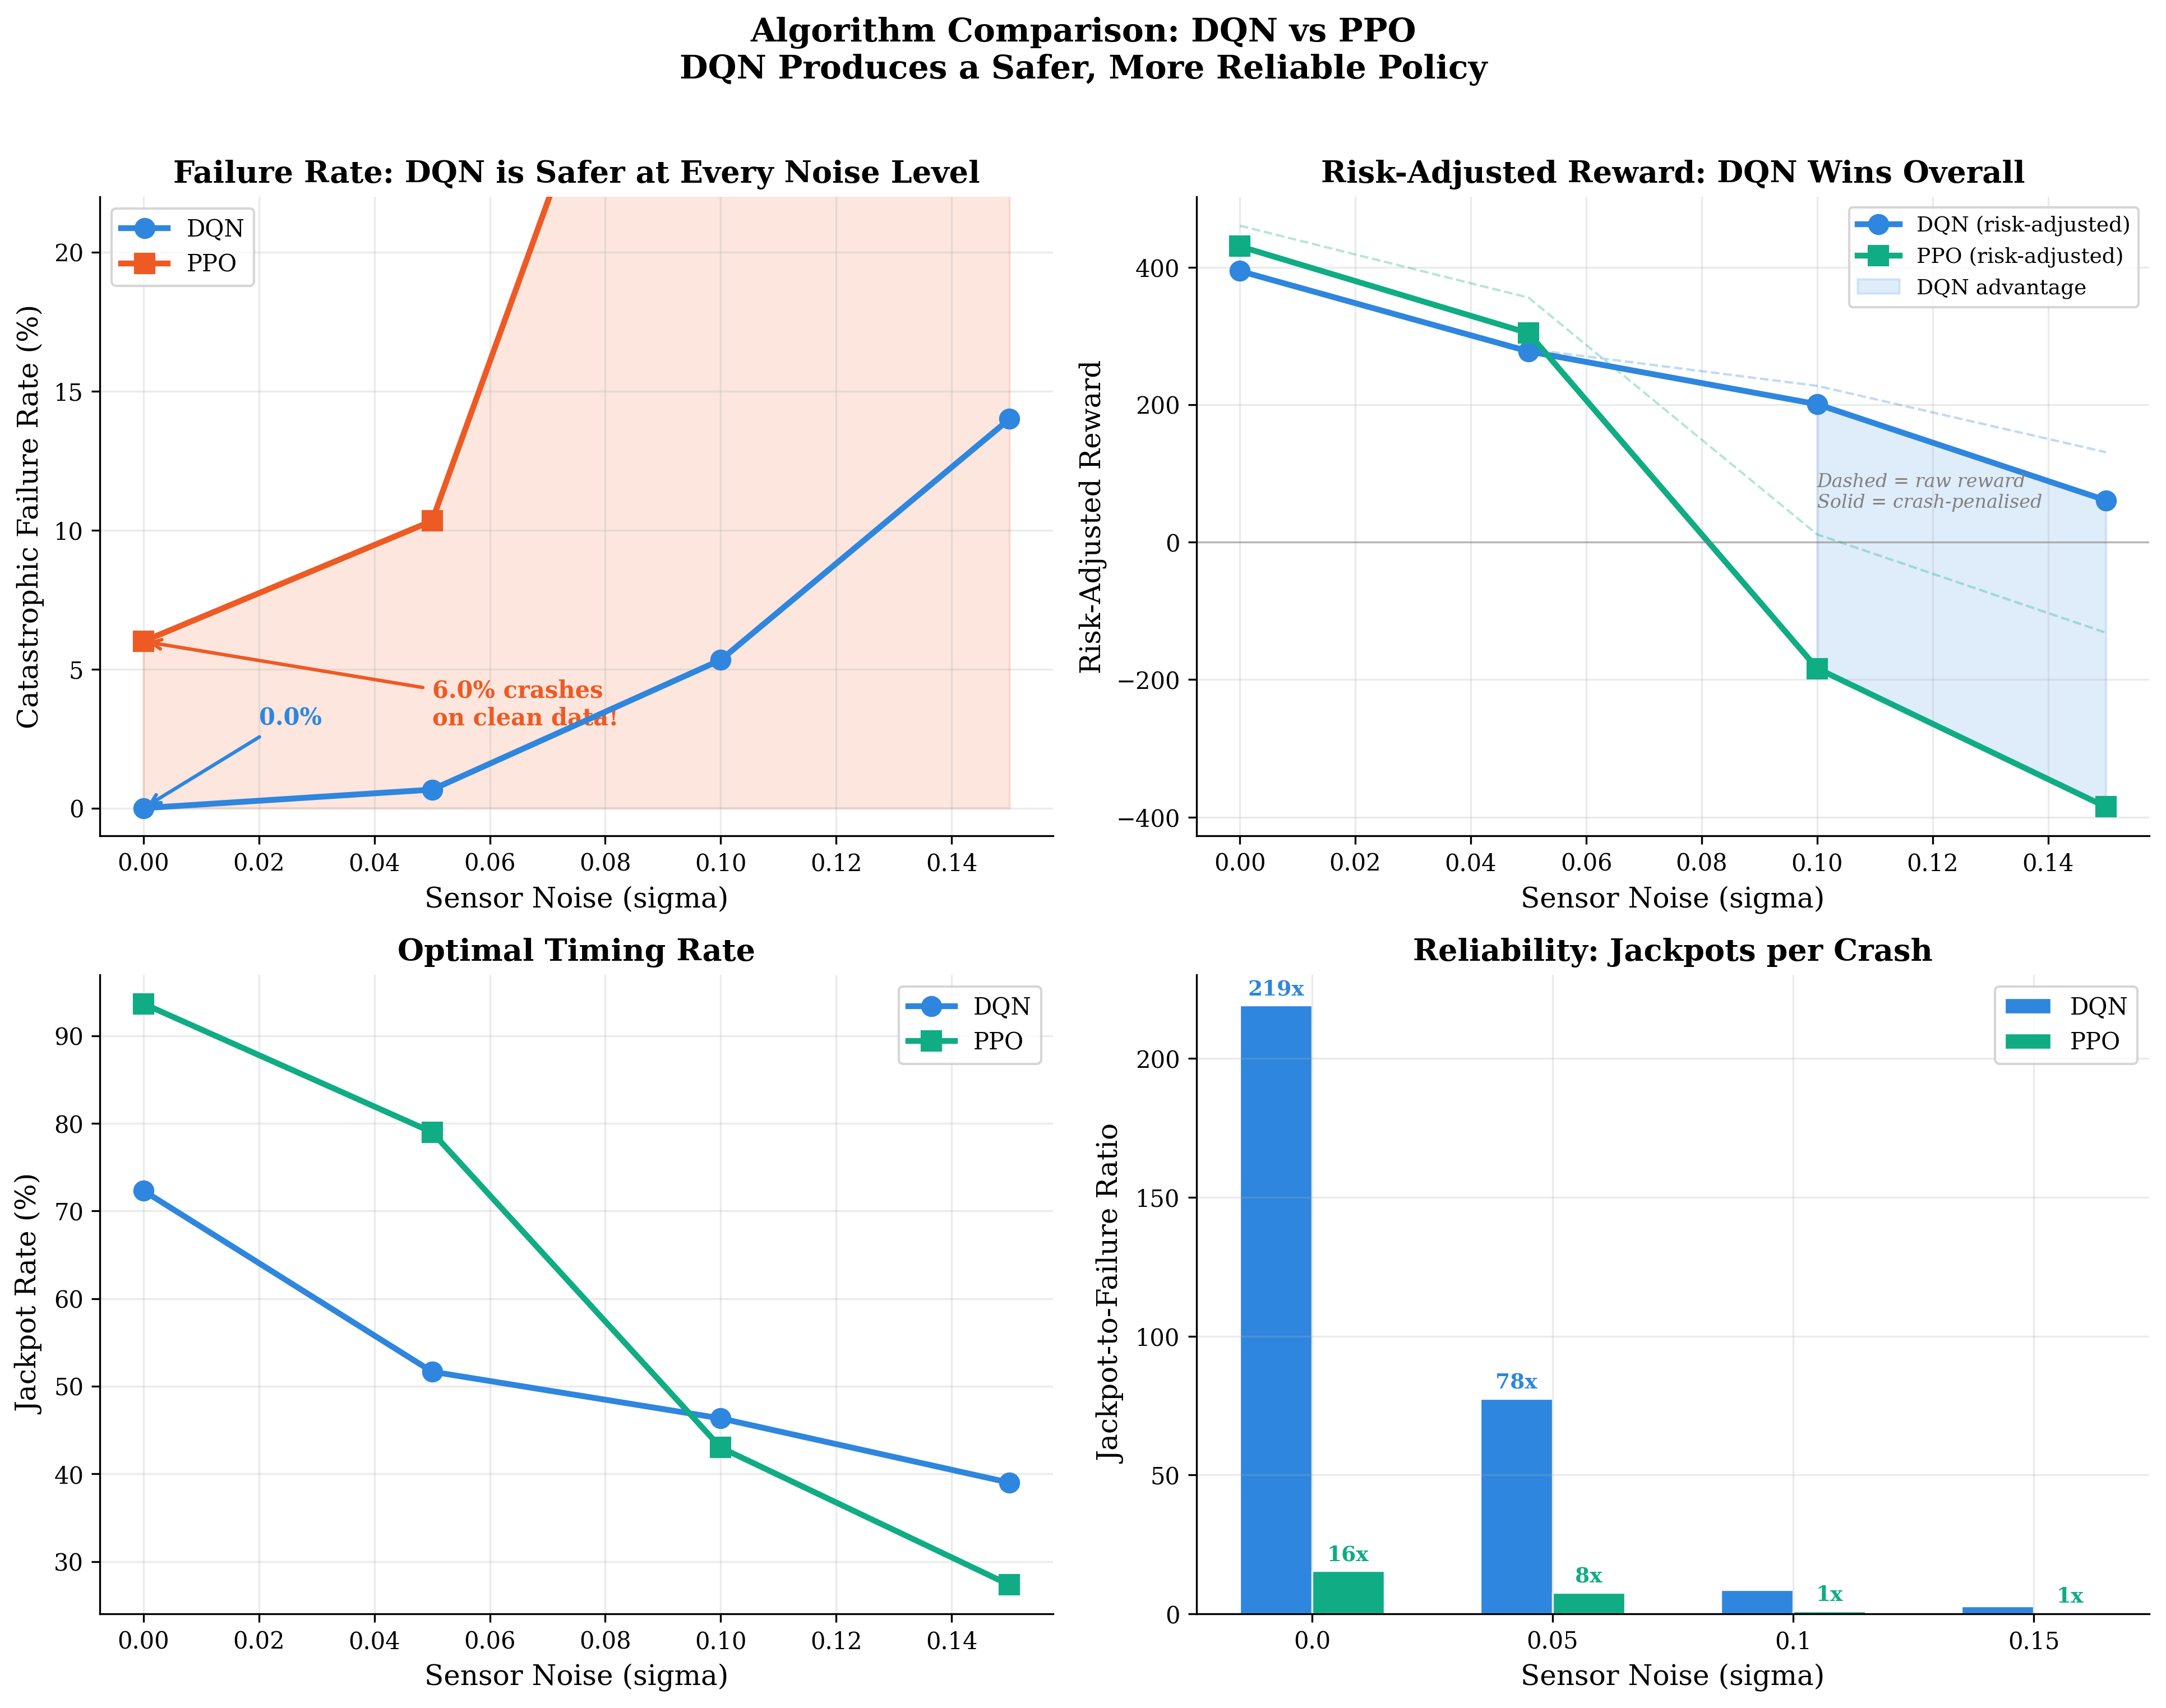
\includegraphics[width=0.95\textwidth]{report_ppo_vs_dqn.png}
\caption{Algorithm comparison: DQN vs PPO across four noise levels (no safety supervisor). Top-left: DQN maintains lower failure rates at every noise level. Top-right: risk-adjusted reward (crash-penalised at $-500$) shows DQN winning decisively. Bottom-left: PPO achieves higher jackpot rates but at unacceptable safety cost. Bottom-right: DQN's jackpot-to-failure ratio is dramatically higher, demonstrating superior reliability.}
\label{fig:ppo_comparison}
\end{figure}

Figure~\ref{fig:ppo_statistical} summarises the statistical analysis. On raw reward, effect sizes are small to negligible ($|d| < 0.36$), indicating comparable learning capacity between algorithms. However, the risk-adjusted comparison (left panel) reveals DQN's true advantage: $+384$ on clean data and $+301$ at $\sigma = 0.1$. The head-to-head scorecard confirms DQN wins three of five key metrics, including the two that matter most for deployment --- failure rate and risk-adjusted reward.

\begin{figure}[h]
\centering
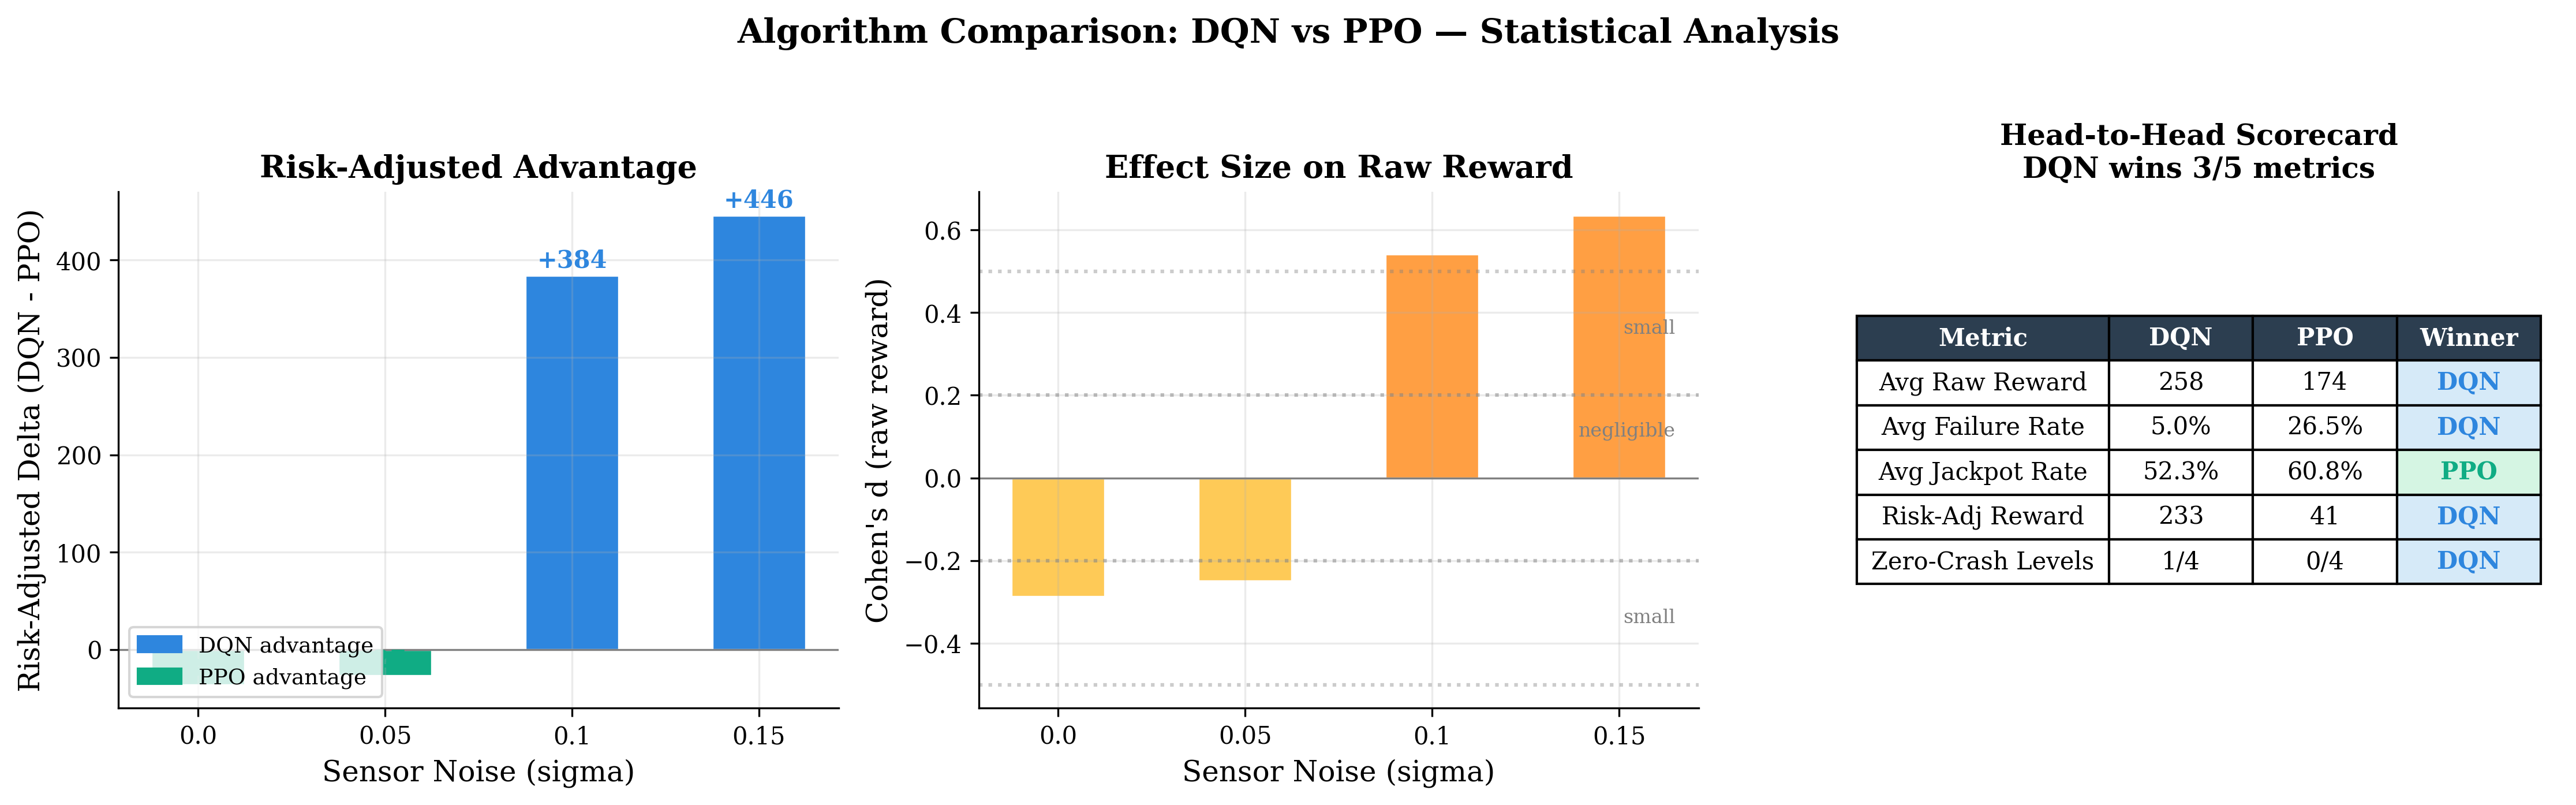
\includegraphics[width=0.95\textwidth]{report_ppo_statistical.png}
\caption{Statistical analysis of DQN vs PPO. Left: risk-adjusted reward delta (DQN $-$ PPO), with DQN advantaged at all noise levels when crash penalties are included. Centre: Cohen's $d$ on raw reward, showing small to negligible effect sizes. Right: head-to-head scorecard --- DQN wins 3/5 metrics including failure rate and risk-adjusted reward.}
\label{fig:ppo_statistical}
\end{figure}

\chapter{Key Source Code}
\label{app:source_code}

This appendix presents excerpts from the most critical source files. The complete codebase is available in the project submission.

\section*{C.1 LSTM Model Architecture}

\begin{verbatim}
class RUL_LSTM(nn.Module):
    def __init__(self, input_dim, hidden_dim, num_layers,
                 output_dim=1, dropout=0.2):
        super(RUL_LSTM, self).__init__()
        self.hidden_dim = hidden_dim
        self.num_layers = num_layers
        self.lstm = nn.LSTM(
            input_size=input_dim,
            hidden_size=hidden_dim,
            num_layers=num_layers,
            dropout=dropout,
            batch_first=True
        )
        self.fc = nn.Linear(hidden_dim, output_dim)

    def forward(self, x):
        out, _ = self.lstm(x)
        out = self.fc(out[:, -1, :])
        return out.squeeze(-1)
\end{verbatim}

\section*{C.2 Gymnasium Environment Observation}

The four-dimensional observation vector is constructed from the ensemble predictions:

\begin{verbatim}
def _get_observation(self):
    unit_data = self.df[self.df['unit'] == self.current_unit]
    start_idx = self.current_time - WINDOW_SIZE
    end_idx = self.current_time
    features = [c for c in unit_data.columns
                if c not in ['unit', 'time', 'RUL']]
    seq = unit_data.iloc[start_idx:end_idx][features].values.copy()

    if self.episode_noisy:
        noise = np.random.normal(0, self.episode_noise_level,
                                 seq.shape)
        seq = np.clip(seq + noise, 0, 1)

    seq_tensor = torch.FloatTensor(seq).unsqueeze(0).to(DEVICE)
    preds = []
    with torch.no_grad():
        for model in self.models:
            preds.append(model(seq_tensor).item())

    norm_mean = np.clip(np.mean(preds), 0, 1)
    norm_std = np.clip(np.std(preds) * UNCERTAINTY_SCALE, 0, 1)
    sensor_trend = np.clip(np.mean(seq[-1, :]), 0, 1)

    self.sigma_history.pop(0)
    self.sigma_history.append(float(norm_std))
    rolling_sigma = float(np.mean(self.sigma_history))

    return np.array([norm_mean, norm_std, rolling_sigma,
                     sensor_trend], dtype=np.float32)
\end{verbatim}

\section*{C.3 Safety Supervisor Logic}

\begin{verbatim}
def safety_override(action, obs):
    if action == 0:  # Only override WAIT decisions
        # Tier 1: Hard critical -- always fire at extreme proximity
        if obs[0] < HARD_CRITICAL_RUL_NORM:
            return 1, True

        # Tier 2: Uncertainty-aware -- fire only when confident
        is_confident = obs[2] < SUPERVISOR_SIGMA_THRESHOLD
        if obs[0] < CRITICAL_RUL_NORM and is_confident:
            return 1, True

    return action, False
\end{verbatim}

\section*{C.4 Reward Function}

\begin{verbatim}
# Inside step() method of PdMEnvironment
if action == 1:  # MAINTAIN
    sigma = getattr(self, '_current_sigma', 0.0)
    proactive_bonus = 0
    if sigma > 0.5 and current_norm_rul < NORM_BUFFER:
        proactive_bonus = 30

    if current_norm_rul < NORM_REPAIR:    # < 20/125
        reward = 500 + proactive_bonus    # Jackpot
    elif current_norm_rul < NORM_BUFFER:  # < 50/125
        reward = 10 + proactive_bonus     # Safe
    else:
        reward = -20                      # Wasteful
    terminated = True

else:  # WAIT
    self.current_time += 1
    if self.current_time >= self.max_time:
        reward = CRASH_PENALTY  # -500
        terminated = True
    else:
        time_pressure = max(0.0,
            (TIME_PRESSURE_START - current_true_rul) / 10.0)
        sigma = getattr(self, '_current_sigma', 0.0)
        uncertainty_urgency = sigma * max(0.0,
            (TIME_PRESSURE_START - current_true_rul) / 3.0)
        reward = 1.0 - time_pressure - uncertainty_urgency
\end{verbatim}

\section*{C.5 DQN Training Configuration}

\begin{verbatim}
from stable_baselines3 import DQN

model = DQN(
    "MlpPolicy", env,
    learning_rate=0.0003,
    buffer_size=150000,
    learning_starts=10000,
    batch_size=128,
    gamma=0.99,
    exploration_fraction=0.4,
    exploration_final_eps=0.03,
    target_update_interval=1000,
    train_freq=4,
    policy_kwargs=dict(net_arch=[256, 256, 128]),
    verbose=1
)
model.learn(total_timesteps=1_500_000)
\end{verbatim}



\chapter{Hyperparameter Configuration}
\label{app:hyperparams}

Table~\ref{tab:app_lstm_params} and Table~\ref{tab:app_rl_params} present the complete set of hyperparameters used in the system, centralised in \texttt{src/config.py}.

\section*{D.1 LSTM Ensemble Hyperparameters}

\begin{table}[h]
\centering
\caption{LSTM deep ensemble training hyperparameters.}
\label{tab:app_lstm_params}
\begin{tabular}{llr}
\toprule
\textbf{Category} & \textbf{Parameter} & \textbf{Value} \\
\midrule
Architecture & Input dimension & 24 \\
 & Hidden dimension & 100 \\
 & Number of LSTM layers & 2 \\
 & Dropout rate & 0.2 \\
 & Ensemble size & 5 \\
\midrule
Training & Epochs & 80 \\
 & Learning rate & 0.0005 \\
 & Batch size & 64 \\
 & Early stopping patience & 15 \\
 & Gradient clipping & 1.0 \\
 & Bootstrap ratio & 0.8 \\
 & Train/validation split & 80/20 \\
\midrule
Data & Window size & 30 \\
 & RUL cap & 125 cycles \\
 & Normalisation range & [0, 1] \\
 & Sensors retained & All 21 \\
 & Settings retained & All 3 \\
\bottomrule
\end{tabular}
\end{table}

\section*{D.2 DQN Agent and RL Environment Hyperparameters}

\begin{table}[h]
\centering
\caption{DQN agent and Gymnasium environment hyperparameters.}
\label{tab:app_rl_params}
\begin{tabular}{llr}
\toprule
\textbf{Category} & \textbf{Parameter} & \textbf{Value} \\
\midrule
DQN Agent & Total timesteps & 1,500,000 \\
 & Network architecture & [256, 256, 128] \\
 & Learning rate & 0.0003 \\
 & Batch size & 128 \\
 & Replay buffer size & 150,000 \\
 & Learning starts & 10,000 \\
 & Exploration fraction & 0.4 \\
 & Final exploration rate & 0.03 \\
 & Target network update interval & 1,000 \\
 & Training frequency & Every 4 steps \\
 & Discount factor ($\gamma$) & 0.99 \\
\midrule
Noise Augmentation & Noise probability & 0.7 \\
 & Noise range ($\sigma$) & [0.02, 0.20] \\
 & Uncertainty scale factor & 15.0 \\
\midrule
Safety Supervisor & Critical RUL threshold & 0.12 ($\approx$15 cycles) \\
 & Hard-critical RUL threshold & 0.04 ($\approx$5 cycles) \\
 & Sigma confidence threshold & 0.55 \\
\midrule
Episode Sampling & End-of-life bias probability & 0.6 \\
 & End-of-life window & 50 cycles \\
\midrule
Reward Function & Jackpot bonus (RUL $< 20$) & +500 \\
 & Safe maintenance (RUL $< 50$) & +10 \\
 & Wasteful maintenance & $-$20 \\
 & Crash penalty & $-$500 \\
 & Time pressure start & 25 cycles \\
 & WAIT base reward & +1.0 \\
\bottomrule
\end{tabular}
\end{table}


\chapter{Additional Visualisations}
\label{app:visualisations}

Appendix~\ref{app:visualisations} presents supplementary figures that provide additional perspectives on the experimental results while keeping primary evidence in the main body. Figure~\ref{fig:app_exp1_alt} shows the Layer~2 ablation from an alternative angle, Figure~\ref{fig:app_exp2_alt} provides an alternative view of full-system performance, and Figure~\ref{fig:app_cost_exec} provides the executive financial projection companion to the main cost-effectiveness figure (Figure~\ref{fig:cost_analysis_main}).

\begin{figure}[h]
    \centering
    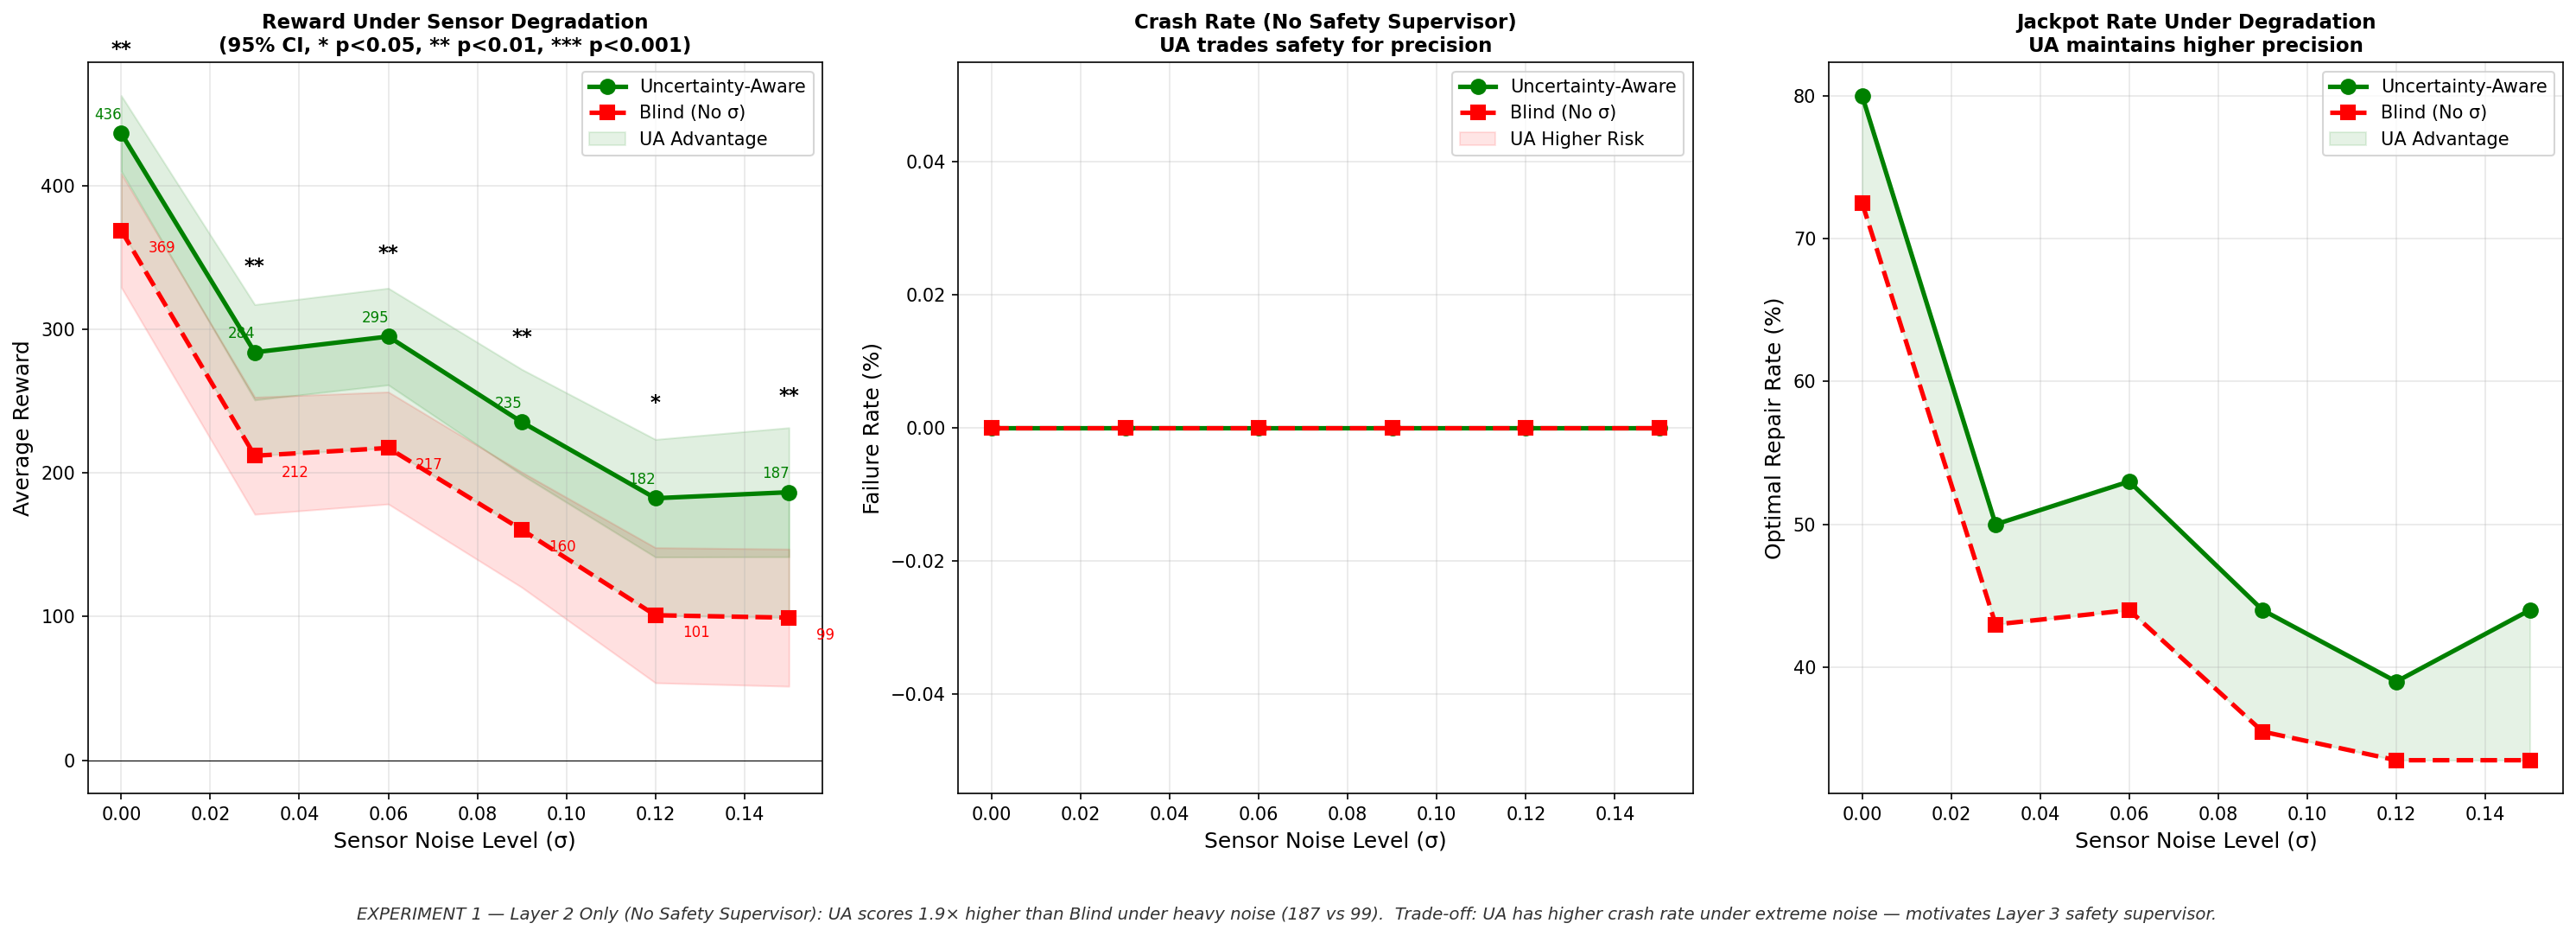
\includegraphics[width=0.85\textwidth]{experiment_1_layer2_ablation.png}
    \caption{Experiment 1 Layer 2 ablation: supplementary visualisation of UA vs Blind reward distributions across all noise levels without the safety supervisor (primary result in Figure~\ref{fig:exp1_chart}).}
    \label{fig:app_exp1_alt}
\end{figure}

\begin{figure}[h]
    \centering
    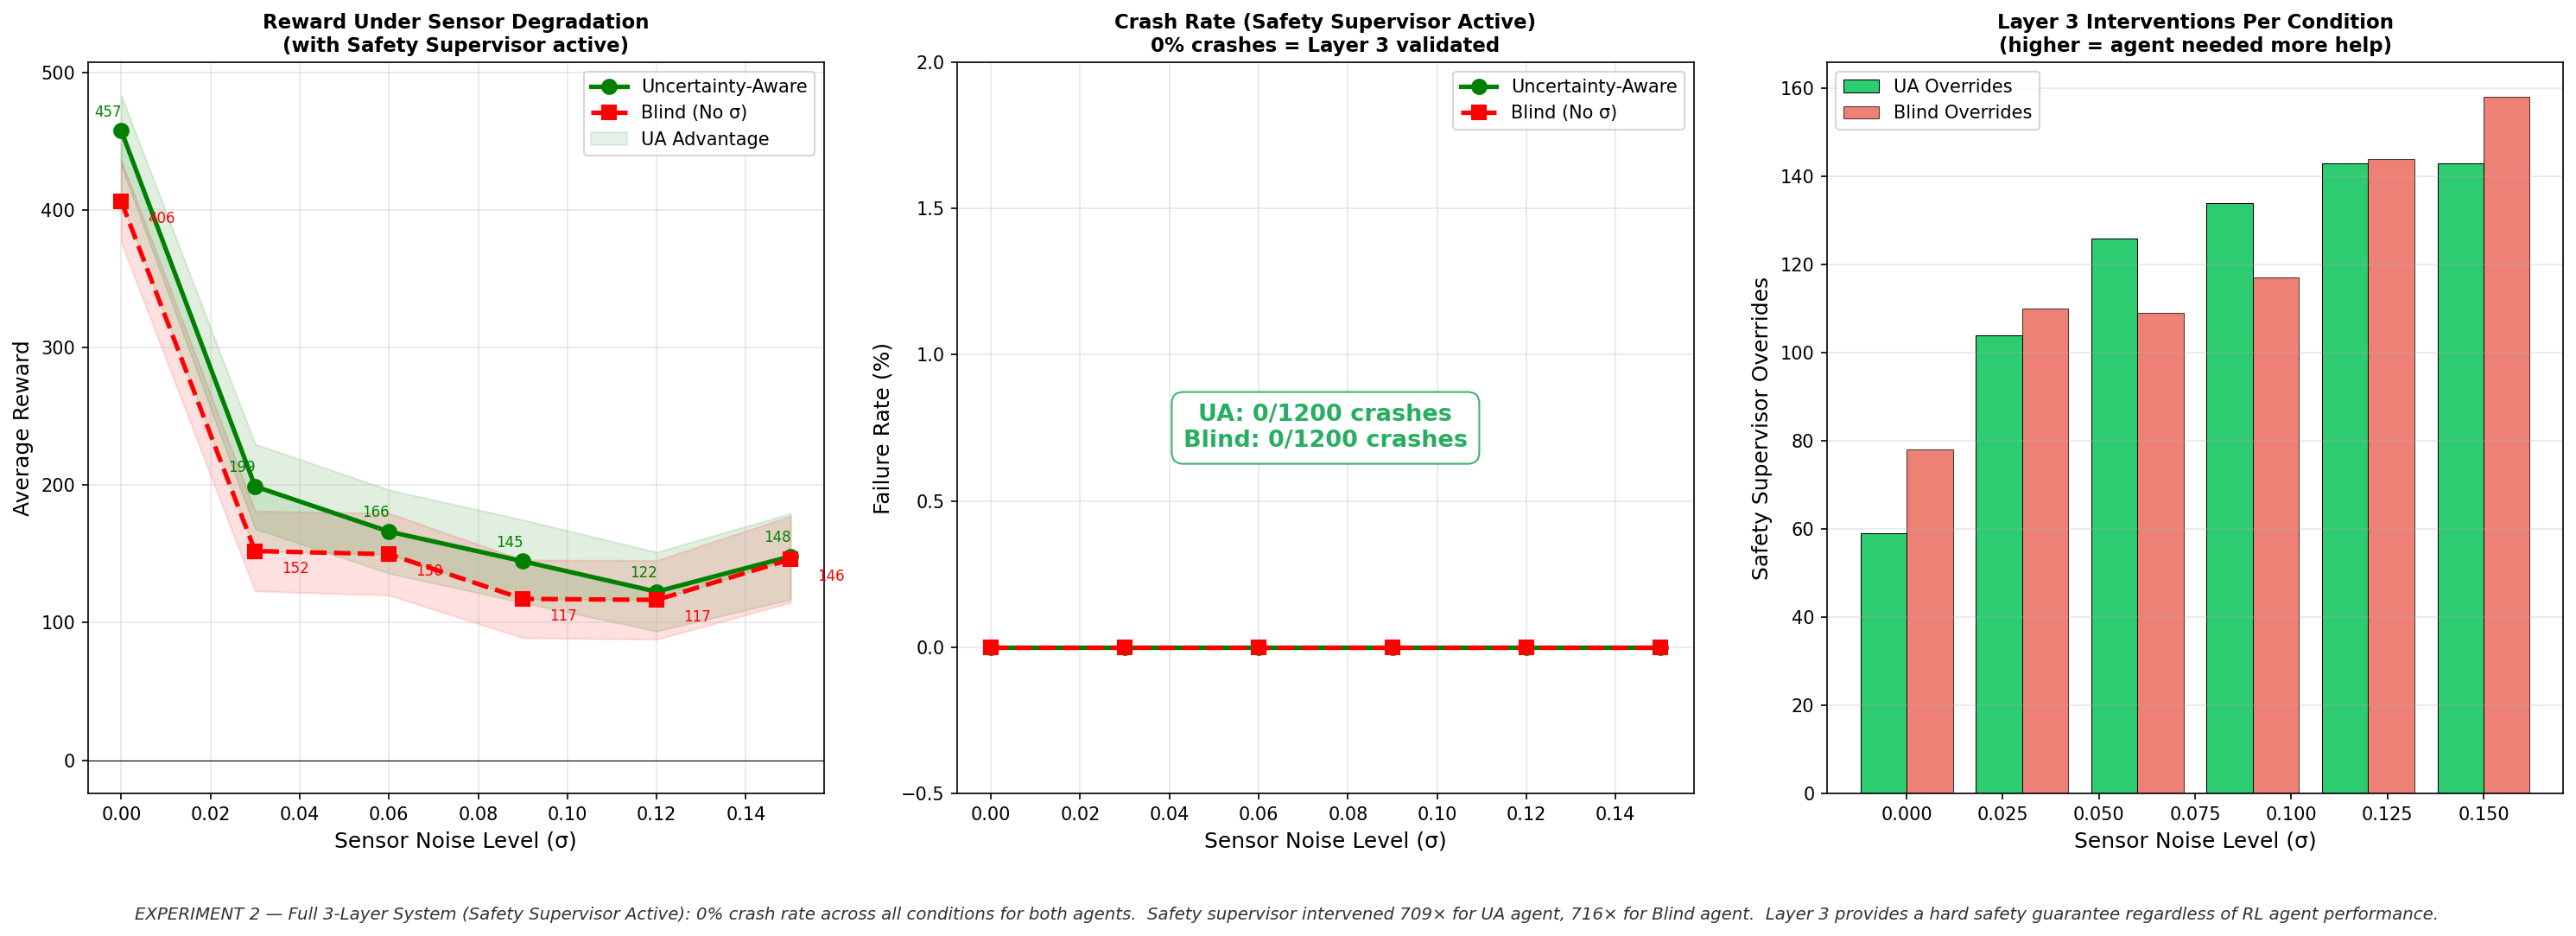
\includegraphics[width=0.85\textwidth]{experiment_2_full_system.png}
    \caption{Experiment 2 full system: supplementary visualisation of UA vs Blind performance with the three-layer safety supervisor active (primary result in Figure~\ref{fig:exp2_chart}).}
    \label{fig:app_exp2_alt}
\end{figure}

\begin{figure}[h]
    \centering
    
\includegraphics[width=0.9\textwidth]{report_cost_executive_summary.png}
    \caption{Executive five-year cost projection for the representative 50-engine fleet, comparing cumulative UA and blind maintenance expenditure.}
    \label{fig:app_cost_exec}
\end{figure}

\section*{E.1 Visualisation Inventory and Provenance}

Table~\ref{tab:app_visual_inventory} maps each generated analysis figure to its producing script, providing a complete audit trail of visual evidence included in this dissertation.

\begin{table}[h]
\centering
\small
\caption{Complete inventory of generated analysis figures and source scripts.}
\label{tab:app_visual_inventory}
\begin{tabular}{>{\raggedright\arraybackslash}p{0.28\textwidth} >{\raggedright\arraybackslash}p{0.66\textwidth}}
\toprule
\textbf{Script} & \textbf{Generated Figures} \\
\midrule
\path{main_evaluate_ensemble.py} & \path{ensemble_evaluation_1_prediction.png}, \path{ensemble_evaluation_2_error.png}, \path{ensemble_evaluation_3_uncertainty.png} \\
\path{main_visualize.py} & \path{uncertainty_vs_error.png}, \path{report_summary_dashboard.png}, \path{final_engine_50_timeline.png}, \path{final_engine_134_timeline.png}, \path{final_engine_200_timeline.png} \\
\path{main_experiment_ablation.py} & \path{report_exp1_layer2_isolation.png}, \path{report_exp2_full_system.png}, \path{report_exp3_safety_contribution.png} \\
\path{main_experiment_threshold.py} & \path{experiment_3_threshold_baseline.png} \\
\path{main_experiment_final.py} & \path{final_result_chart.png}, \path{experiment_1_layer2_ablation.png}, \path{experiment_2_full_system.png} \\
\path{main_cost_analysis.py} & \path{report_cost_analysis.png}, \path{report_cost_executive_summary.png} \\
\path{main_experiment_ppo.py} & \path{report_ppo_vs_dqn.png} \\
\path{generate_charts.py} & \path{report_ppo_statistical.png}, \path{report_test_results.png} \\
\bottomrule
\end{tabular}
\end{table}


\chapter{Testing Documentation}
\label{app:testing}

\section*{F.1 Automated Test Suite}

An automated test suite (\texttt{test\_system.py}) was developed using the \texttt{pytest} framework, comprising 29 test cases across six test classes. The full suite can be executed with \texttt{pytest test\_system.py -v} and completed in approximately 20 seconds on the development machine. All 29 tests passed on the final codebase (29/29 pass, 0 failures). The test classes cover:

\begin{itemize}
    \item \textbf{TestDataPipeline} (5 tests): Data loading, column count, RUL cap, NaN-free normalisation, FD002 unit ID offset.
    \item \textbf{TestLSTMModel} (4 tests): Output shape, output range, model loading, ensemble diversity (non-zero standard deviation across members).
    \item \textbf{TestEnvironment} (7 tests): 4D observation shape and range, WAIT time advancement, MAINTAIN episode termination, noise injection increasing sigma, blind environment zeroing sigma.
    \item \textbf{TestRewardFunction} (4 tests): Correct classification of jackpot, crash, safe, and wasteful terminal rewards including proactive bonus variants.
    \item \textbf{TestSafetySupervisor} (6 tests): Tier 1 fires at hard-critical RUL, Tier 2 fires when confident, Tier 2 backs off under high uncertainty, no override at safe RUL, no override on MAINTAIN action, blind agent always triggers Tier 2.
    \item \textbf{TestIntegration} (3 tests): Full episode completion, fixed-seed reproducibility, trained DQN agent loading and action prediction.
\end{itemize}

Table~\ref{tab:unit_test_results} summarises the automated test outcomes by class, as reported by \texttt{pytest}.

\begin{table}[h]
\centering
\small
\caption{Automated test results by test class (\texttt{pytest test\_system.py -v}). All tests executed on the final codebase with trained model artefacts present.}
\label{tab:unit_test_results}
\renewcommand{\arraystretch}{1.3}
\begin{tabular}{lrl}
\toprule
\textbf{Test Class} & \textbf{Cases} & \textbf{Result} \\
\midrule
\texttt{TestDataPipeline}: loading, RUL cap, normalisation, unit offset & 5 & 5/5 Pass \\
\texttt{TestLSTMModel}: shape, range, loading, diversity & 4 & 4/4 Pass \\
\texttt{TestEnvironment}: observations, actions, noise, blind variant & 7 & 7/7 Pass \\
\texttt{TestRewardFunction}: jackpot, crash, safe, wasteful classification & 4 & 4/4 Pass \\
\texttt{TestSafetySupervisor}: Tier 1, Tier 2, $\sigma$ gate, edge cases & 6 & 6/6 Pass \\
\texttt{TestIntegration}: episode completion, reproducibility, agent loading & 3 & 3/3 Pass \\
\midrule
\multicolumn{1}{r}{\textbf{Total}} & \textbf{29} & \textbf{29/29 Pass} \\
\bottomrule
\end{tabular}
\end{table}

Figure~\ref{fig:test_results} visualises the test distribution across system components. The suite achieves coverage of all three architectural layers, with the heaviest testing concentrated on the environment (Layer~2) and safety supervisor (Layer~3): the two components where correctness is most critical for safe operation.

\begin{figure}[h]
\centering

\includegraphics[width=0.95\textwidth]{report_test_results.png}
\caption{Automated test suite summary. Left: test case counts by class, with all 29 cases passing. Right: coverage distribution by system component, showing emphasis on the decision layer (28\%) and safety supervisor (24\%).}
\label{fig:test_results}
\end{figure}

\section*{F.2 Integration Testing}

Integration testing was performed by running short training sessions (10,000 timesteps) and verifying that:

\begin{itemize}
    \item The ensemble models load correctly and produce consistent predictions.
    \item Noise injection modifies observations as expected (higher sigma under noisy conditions).
    \item The safety supervisor fires at the correct thresholds.
    \item The DQN agent's replay buffer stores transitions in the correct format.
    \item The reward function returns correct values for each action-state combination.
\end{itemize}

The automated test suite also includes integration-level checks (Table~\ref{tab:integration_test_results}). Additional manual integration checks were performed during development, as documented below.

\begin{table}[h]
\centering
\small
\caption{Integration and system-level verification checks, combining automated (\texttt{pytest}) and manual validation.}
\label{tab:integration_test_results}
\renewcommand{\arraystretch}{1.3}
\begin{tabular}{lrl}
\toprule
\textbf{Test Scenario} & \textbf{Method} & \textbf{Result} \\
\midrule
Full episode completes without error & \texttt{pytest} & Pass \\
Fixed seed produces identical trajectories & \texttt{pytest} & Pass \\
Trained DQN loads and produces valid actions & \texttt{pytest} & Pass \\
Noise injection: $\sigma$ increases with noise level & \texttt{pytest} & Pass \\
Blind env: override count $\gg$ UA override count & Manual (200 eps) & Pass \\
DQN short training (10K steps): loss decreases, no NaN & Manual & Pass \\
Full pipeline: train $\rightarrow$ save $\rightarrow$ reload $\rightarrow$ eval & Manual & Pass \\
\midrule
\multicolumn{2}{r}{\textbf{Total}} & \textbf{7/7 Pass} \\
\bottomrule
\end{tabular}
\end{table}

\section*{F.3 Statistical Validation}

All experimental comparisons used the following statistical protocol:

\begin{itemize}
    \item \textbf{Sample size:} 500 episodes per agent per noise level (1,000 episodes per comparison).
    \item \textbf{Hypothesis test:} Welch's unequal-variance $t$-test (two-tailed).
    \item \textbf{Significance levels:} * ($p < 0.05$), ** ($p < 0.01$), *** ($p < 0.001$).
    \item \textbf{Effect size:} Cohen's $d$ with thresholds: negligible ($< 0.2$), small ($0.2$--$0.5$), medium ($0.5$--$0.8$), large ($\geq 0.8$).
    \item \textbf{Confidence intervals:} 95\% CI computed as $\bar{x} \pm 1.96 \cdot \frac{s}{\sqrt{n}}$.
    \item \textbf{Total episodes:} 8,000 per experiment $\times$ 3 experiments $=$ 24,000 episodes.
\end{itemize}

\section*{F.4 Dashboard Usability Testing}

The Streamlit dashboard (Section~4.7) was tested manually by the author and demonstrated to the project supervisor during a scheduled feedback session. The following checks were performed:

\begin{itemize}
    \item Running cycle-by-cycle simulations for multiple engines under varying noise levels.
    \item Verifying that the live Plotly charts update correctly at each cycle.
    \item Confirming that the UA/Blind toggle and safety supervisor toggle produce expected behavioural differences.
    \item Checking that session state persists correctly across Streamlit reruns.
    \item Testing the noise injection slider across its full range and verifying that uncertainty estimates respond proportionally.
\end{itemize}

The supervisor demonstration confirmed that the interface clearly communicated the system's decision-making process and that the three-panel visualisation made the interaction between prediction uncertainty and agent behaviour intuitive to a non-specialist observer. The primary feedback received was to ensure the status panel clearly distinguished between agent-initiated and supervisor-initiated maintenance actions, which was implemented in the final version through colour-coded status indicators.

\section*{F.5 Reproducibility Runbook (All Tests and Plots)}

The following command sequence reproduces the complete evaluation and plotting pipeline from a clean environment:

\begin{verbatim}
pytest test_system.py -v              # Automated test suite (29 tests)
python main_evaluate_ensemble.py
python main_experiment_ablation.py
python main_experiment_threshold.py
python main_experiment_final.py
python main_experiment_ppo.py         # PPO vs DQN comparison
python main_cost_analysis.py
python main_visualize.py
python main_evaluate.py
\end{verbatim}

The generated outputs include all figures referenced in Chapters~4--5 and Appendix~\ref{app:visualisations}, as well as CSV artefacts (\path{report_experiment_results.csv} and \path{report_cost_summary.csv}) used for numerical validation.




\chapter{Extended Implementation Details}
\label{app:impl_details}

This appendix provides the detailed implementation descriptions that support the summary presented in Chapter~4.

\section*{G.1 Data Pipeline Details}

The preprocessing module assigned standard column names (unit ID, cycle number, three operational settings, and 21 sensor measurements) and loaded both FD001 and FD002 files into a single DataFrame. Because both subsets used independent unit numbering starting from 1, FD002 unit IDs were offset by the maximum FD001 unit ID (100) to prevent collisions. Without this offset, the sliding-window generator would have created sequences that incorrectly spanned two different engines at the boundary.

RUL was computed as the difference between each engine's final cycle and the current cycle, capped at 125 following \citet{heimes2008recurrent}. All 24 features were scaled to $[0, 1]$ using MinMaxScaler, with the fitted scaler serialised for consistent inference. No sensors were dropped because FD002's six operating conditions cause all three settings to vary meaningfully. The sliding-window generator extracted windows of $30 \times 24$ features paired with the normalised RUL at the window's final cycle, producing approximately 46,000 training sequences.

\section*{G.2 LSTM Ensemble Training Details}

Each ensemble member was trained on a random 80\% subset drawn without replacement (seed = 42 + $i \times 17$), with the remaining 20\% serving as validation. This follows \citet{fort2019deep}, who showed that training data diversity combined with random initialisation produces meaningful disagreement. Sampling without replacement produced tighter validation loss distributions while maintaining sufficient diversity.

The architecture (two-layer LSTM, hidden dimension 100, dropout 0.2, linear output) was deliberately kept simple because the primary contribution was uncertainty propagation, not prediction accuracy. Training used Adam ($\text{lr} = 5 \times 10^{-4}$), MSE loss, ReduceLROnPlateau scheduling (halving after 5 epochs without improvement), early stopping (patience 15), and gradient clipping at 1.0. Most models converged within 40--60 epochs.

\section*{G.3 Implementation Challenges: Extended Discussion}

\textbf{End-of-life class imbalance.} Finding the correct balance (60\% biased episodes, 50-cycle window) required several iterations. Too little bias left the agent undertrained on critical decisions; too much caused over-triggering in the healthy phase. The final values were determined through systematic sweeps.

\textbf{Uncertainty scale calibration.} The UNCERTAINTY\_SCALE factor of 15 was calibrated so that clean-data uncertainty mapped to approximately 0.15--0.30, moderate noise to 0.50--0.60, and heavy noise to 0.80+, providing clear separation. This calibration directly informed the safety supervisor's confidence threshold (0.55).

\textbf{Crash penalty magnitude.} With $\gamma = 0.99$, the initial $-100$ penalty had a present value of only $-20$ at 160 steps, easily outweighed by accumulated WAIT rewards. Increasing to $-500$ raised the present value to approximately $-100$, making crash avoidance material from early degradation stages.

\section*{G.4 Performance Benchmarks}

Table~\ref{tab:app_perf_benchmarks} reports measured wall-clock times for the key computational stages. All timings were recorded on a single consumer machine (Intel i7 CPU, NVIDIA GTX-series GPU, 16\,GB RAM) running Windows 11. Ensemble inference comfortably satisfied the NF2 requirement of sub-100\,ms per cycle, confirming that the system could operate in a real-time decision loop.

\begin{table}[h]
\centering
\small
\caption{Wall-clock performance benchmarks for the major computational stages.}
\label{tab:app_perf_benchmarks}
\renewcommand{\arraystretch}{1.3}
\begin{tabular}{llr}
\toprule
\textbf{Stage} & \textbf{Description} & \textbf{Time} \\
\midrule
Data loading \& preprocessing & Load FD001+FD002, normalise, generate windows & $\sim$8\,s \\
LSTM ensemble training & 5 models $\times$ 80 epochs (early stop $\sim$50) & $\sim$25\,min (GPU) \\
DQN agent training (UA) & 1.5M timesteps with noise augmentation & $\sim$40\,min (CPU) \\
DQN agent training (Blind) & 1.5M timesteps without noise augmentation & $\sim$35\,min (CPU) \\
\midrule
Ensemble inference (1 cycle) & 5 forward passes + $\sigma$ computation & $\sim$12\,ms (GPU) \\
Ensemble inference (1 cycle) & Same, CPU fallback & $\sim$38\,ms (CPU) \\
DQN action selection (1 cycle) & Single forward pass through Q-network & $<$1\,ms \\
Safety supervisor check & Two threshold comparisons & $<$0.01\,ms \\
Full pipeline per cycle & Ensemble + DQN + supervisor & $\sim$13\,ms (GPU) \\
\midrule
Ablation study (full) & 3 experiments $\times$ 8 noise $\times$ 500 eps & $\sim$75\,min \\
Cost analysis & 50-engine fleet projection & $\sim$2\,s \\
Dashboard (per cycle render) & Ensemble + DQN + Plotly update & $\sim$50\,ms \\
\bottomrule
\end{tabular}
\end{table}

The 13\,ms full-pipeline latency per cycle is well within the 100\,ms requirement (NF2) and would also satisfy tighter real-time constraints in production. The DQN training time of approximately 40 minutes on CPU demonstrates that the system is trainable on commodity hardware, though GPU acceleration would reduce this for larger-scale deployments.

\section*{G.5 Technical Justification of Model Choices}

This section documents the design rationale requested by the supervisory feedback in a structured manner: forecasting backbone choice (LSTM), uncertainty modelling choice (deep ensembles), control paradigm choice (RL), and algorithm choice within RL (DQN over PPO).

\textbf{Why LSTM for RUL forecasting.} RUL prediction from multivariate sensor telemetry is inherently sequential: useful signal depends not only on current readings but also on temporal evolution, lag effects, and degradation trajectory shape. LSTM was selected because gated recurrent memory handles long-range dependencies more robustly than vanilla RNNs \citep{hochreiter1997long}. On C-MAPSS specifically, LSTM-family models have repeatedly shown strong predictive performance and practical robustness \citep{zheng2017long, wu2018remaining, li2018remaining}. Compared with purely statistical regressors or shallow feed-forward networks, LSTM provides a direct mechanism to learn degradation dynamics from windows of sensor history rather than requiring heavy manual feature engineering.


\textbf{Why not use Transformer/CNN as the primary backbone.} Transformer-based prognostics can be highly accurate in large-data regimes \citep{zhang2022transformer}, and CNN-LSTM hybrids are competitive \citep{wang2024adaptive}. However, the project optimised for a three-way balance: (1) stable training on available data, (2) fast repeated inference inside an RL environment, and (3) compatibility with ensemble uncertainty estimation under repeated forward passes. A compact two-layer LSTM provided a better engineering trade-off for this objective than a heavier attention backbone requiring larger optimisation and compute budgets.


\textbf{Why uncertainty modelling was necessary.} Predictive maintenance decisions are safety-relevant; therefore, a point estimate alone is insufficient under sensor degradation. Without uncertainty, the policy cannot distinguish ``confidently low RUL'' from ``possibly low due to noisy input''. This distinction is central in out-of-distribution and shifted-input settings \citep{der2009aleatory, ovadia2019can}. In this project, uncertainty was used as an actionable state variable, not merely a post-hoc confidence display.


\textbf{Why deep ensembles for uncertainty.} Among practical uncertainty methods, deep ensembles were chosen because they are implementation-friendly, parallelisable, and empirically well-calibrated under shift \citep{lakshminarayanan2017simple, ovadia2019can}. Bayesian neural networks offer a stronger formal Bayesian interpretation but are heavier to train and tune in deep sequential settings. MC Dropout is lightweight but can under-estimate epistemic uncertainty in difficult regions \citep{gal2016dropout, osband2016risk}. For the objective of feeding uncertainty into downstream RL decisions, ensemble disagreement provided a robust and interpretable signal:
\begin{equation}
\bar{r}_t = \frac{1}{M}\sum_{m=1}^{M} r_t^{(m)}, \qquad
\sigma_t = \sqrt{\frac{1}{M-1}\sum_{m=1}^{M}\left(r_t^{(m)}-\bar{r}_t\right)^2}
\end{equation}


\textbf{Why reinforcement learning for maintenance control.} The decision problem is sequential and delayed-reward: acting now changes future state trajectories, and the value of waiting depends on future uncertainty and failure risk. Rule-based thresholding can provide safety but lacks adaptive policy learning across heterogeneous trajectories. RL naturally formulates this as maximising expected discounted return in an MDP:
\begin{equation}
\pi^* = \arg\max_{\pi} \; \mathbb{E}_{\pi}\left[\sum_{t=0}^{T} \gamma^t r_t\right]
\end{equation}
This allows direct optimisation of the real objective trade-off between early-maintenance waste and late-maintenance failure risk.


\textbf{Why DQN instead of PPO.} The action space is discrete and binary. In such settings, value-based methods are typically efficient and stable when replay buffers and target networks are used \citep{mnih2015human}. DQN also permits extensive data reuse (off-policy learning), which is valuable when environment rollouts are expensive due to ensemble inference at each step. PPO \citep{schulman2017proximal}, while strong in many continuous-control tasks, is on-policy and therefore discards experience after update epochs, making it less sample-efficient here. For this project scope, DQN provided a better cost-benefit profile for convergence speed, tuning complexity, and reproducibility. The update equations used were:
\begin{equation}
y_t = r_t + \gamma \max_{a'}Q_{\theta^-}(s_{t+1}, a'), \qquad
\mathcal{L}(\theta)=\mathbb{E}\left[(Q_{\theta}(s_t,a_t)-y_t)^2\right]
\end{equation}


\textbf{Summary comparison.} Table~\ref{tab:app_model_justification} summarises the final selection logic.

\begin{table}[h]
\centering
\small
\caption{Model-choice justification summary for core architectural components.}
\label{tab:app_model_justification}
\setlength{\tabcolsep}{4pt}
\begin{tabular}{p{2.6cm} p{3.4cm} p{6.0cm} p{3.0cm}}
\toprule
\textbf{Decision} & \textbf{Chosen option} & \textbf{Primary reason} & \textbf{Alternatives considered} \\
\midrule
Forecasting backbone & LSTM deep ensemble & Strong temporal modelling on C-MAPSS with moderate compute and stable training; supports repeated inference for RL loop & Transformer, CNN-LSTM, SVR \\
Uncertainty method & Deep ensemble disagreement & Better practical calibration under shift and interpretable disagreement signal for policy input & MC Dropout, Bayesian NN \\
Control paradigm & RL (MDP) & Direct optimisation of sequential maintenance timing under delayed rewards & Fixed thresholds, myopic heuristics \\
RL algorithm & DQN & Binary action space and off-policy sample efficiency with replay/target networks & PPO, SAC \\
\bottomrule
\end{tabular}
\end{table}

\section*{G.6 Limitations of the Chosen Design}

Although justified for this project scope, the chosen stack is not universally optimal. LSTM may underperform attention models on larger multi-regime datasets; deep ensembles incur multi-model inference overhead; and DQN can be sensitive to reward shaping and exploration schedules. These limitations are acceptable for the current benchmark-focused objective but motivate future comparative studies with PPO, SAC, and transformer-based prognostics, as already outlined in Chapter~7.


\chapter{Original Contributions}
\label{app:contributions}

This appendix clarifies the boundary between established tools used as building blocks and the novel design decisions, formulations, and integration mechanisms authored as part of this project.

\section*{H.1 Contributions Matrix}

Table~\ref{tab:app_contributions} distinguishes existing libraries and datasets from the original work contributed by this project.

\begin{table}[h]
\centering
\small
\caption{Existing tools vs.\ original contributions.}
\label{tab:app_contributions}
\begin{tabular}{p{5.5cm} p{8.5cm}}
\toprule
\textbf{Used (existing tools)} & \textbf{Designed and built (original contributions)} \\
\midrule
LSTM architecture (PyTorch) & Ensemble uncertainty to RL observation pipeline: routing ensemble disagreement ($\sigma$) as a first-class state variable into the DQN agent \\
\addlinespace
DQN algorithm (Stable-Baselines3) & Uncertainty-aware reward shaping formula: the \path{uncertainty_urgency} term ($\sigma \times \max(0, (25 - \text{RUL}) / 3.0)$) that penalises waiting under high disagreement \\
\addlinespace
Gymnasium environment framework & Noise augmentation training protocol: variable per-episode Gaussian injection ($\sigma \in [0.02, 0.20]$, 70\% probability) to teach the agent what uncertainty means during training \\
\addlinespace
NASA C-MAPSS dataset (FD001 + FD002) & $\sigma$-gated two-tier safety supervisor: confidence-aware override that backs off under high uncertainty (Tier~2) while maintaining an unconditional emergency fallback (Tier~1) \\
\addlinespace
MinMaxScaler (scikit-learn) & End-of-life episode biasing strategy: forcing 60\% of training episodes to start in the final 50 cycles to address sparse-reward imbalance \\
\addlinespace
Plotly / Streamlit (visualisation) & Four-dimensional observation design: $[\mu_{\text{RUL}}, \sigma_{\text{now}}, \sigma_{\text{rolling}}, \text{trend}]$ separating instantaneous vs.\ smoothed uncertainty for robust decision-making \\
\addlinespace
Welch's $t$-test / Cohen's $d$ (SciPy) & Blind ablation methodology: systematic comparison against an architecturally identical agent with $\sigma = 0$ to isolate the value of uncertainty awareness \\
\addlinespace
 & Full three-layer integration architecture: connecting ensemble disagreement through reward shaping, observation design, and safety override into a coherent decision pipeline \\
\addlinespace
 & Cost-effectiveness translation model: mapping RL reward outcomes to real-world fleet maintenance costs (GBP) with override-aware operational costing \\
\bottomrule
\end{tabular}
\end{table}

\section*{H.2 Summary of Original Work}

The individual components (LSTM, DQN, Gymnasium, C-MAPSS) are established tools. The contribution of this project lies in \textit{how} they were connected and \textit{what was designed around them}:

\begin{enumerate}
    \item \textbf{The uncertainty-aware reward function}: no existing library provides the \texttt{uncertainty\_urgency} shaping term. This formulation was designed, calibrated, and validated as part of this project.
    \item \textbf{The noise augmentation training protocol}: the insight that an RL agent must \textit{experience} uncertainty during training to learn from it is a methodological contribution, not a library feature.
    \item \textbf{The $\sigma$-gated safety supervisor}: standard safety overrides use fixed thresholds. The two-tier design with confidence gating (backing off when predictions are unreliable) is a novel mechanism.
    \item \textbf{The end-of-life episode biasing}: addressing the sparse-reward problem by curriculum-style episode sampling is a training design decision specific to this domain.
    \item \textbf{The blind ablation framework}: using an architecturally identical agent with zeroed uncertainty to isolate the exact contribution of $\sigma$-awareness is an experimental design choice, not a library function.
    \item \textbf{The complete integration}: routing ensemble disagreement through observation, reward, and safety override into one coherent pipeline required substantial design effort beyond assembling existing parts.
\end{enumerate}

\noindent The analogy is that of engineering: a civil engineer does not manufacture steel or concrete, but designs the bridge. The libraries are materials; the framework described in this dissertation is the design.

\end{document}
